%\chapter{Real Data}
%Finally, we also performed inference on a real FMRI scan. The scanner we used...
%... more specifics...

% TODO include single?
%Before performing tests on a full image, I the particle filter
%on regions deemed active and inactive by statistical parametric mapping
%(SPM). This served the purpose of adjusting the priors as well as the 
%preprocessing based on real world signals. This was actually done before
%the simulations, and then results were carried back the simulations 
%to check consistency.
%After work adjusting parameters, most importantly the weighting function and the 
%priors, particle filter was applied to every voxel in an FMRI image.
%The results of this large scale analysis was a parameter map which was
%then used to calculate normalized square-root MSE image. 
%
%\section{Single-Voxel Analysis}
%The choice of a prior, as discussed previously, is extremely important. While a
%prior may have the potential to give good results, being a monte-carlo algorithm
%there is the possibility for inconsistencies. Thus, increasing the variance
%of the time-constants may allow additional flexibility, it will also cause
%additional model variance. Before running on a full volume I adjusted the 
%prior to ensure that the same input would give the same output 100 times in a 
%row. While this may seem like a given, with a random drawing of the prior,
%this can be difficult. Case in point, the exact same algorithm run twice
%with the time constants all having standard deviations of $.35$ resulted in two
%very different fits, shown in \autoref{fig:badfit_param1}.
%
%\begin{figure}
%\subfigure{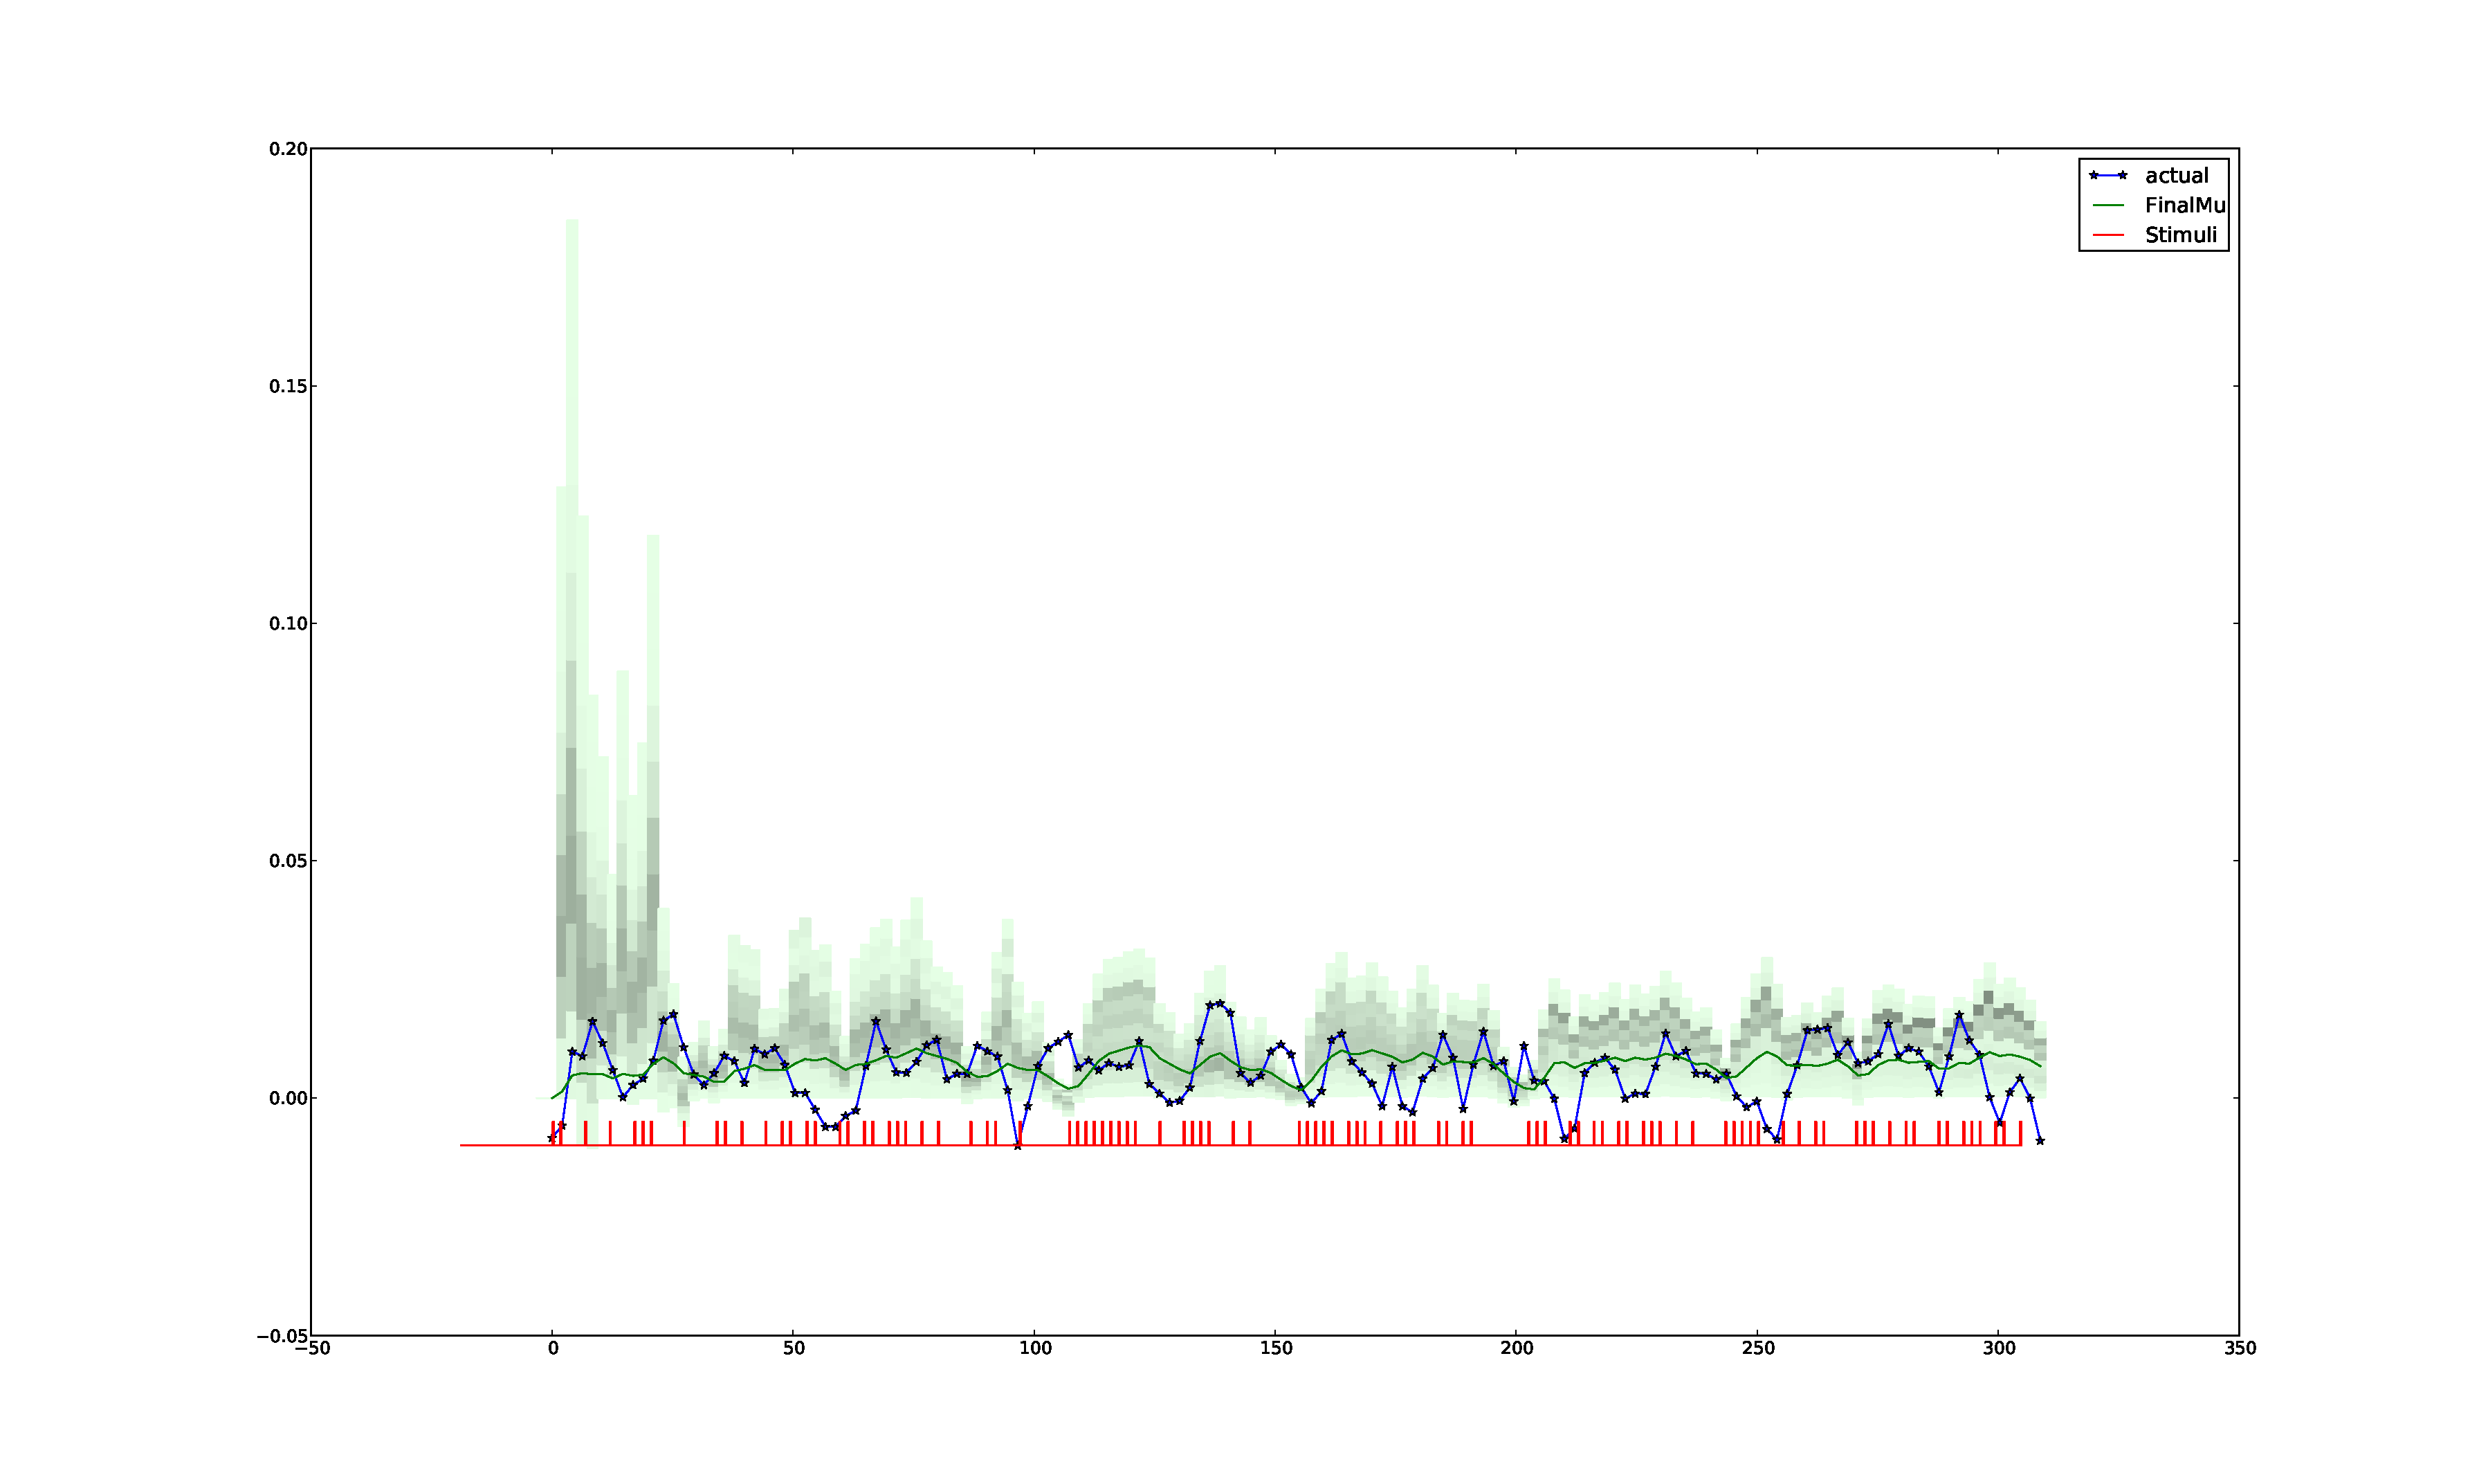
\includegraphics[clip=true,trim=6cm 2cm 6cm 3.5cm,width=17cm]{images/badfit_param1}}
%\subfigure{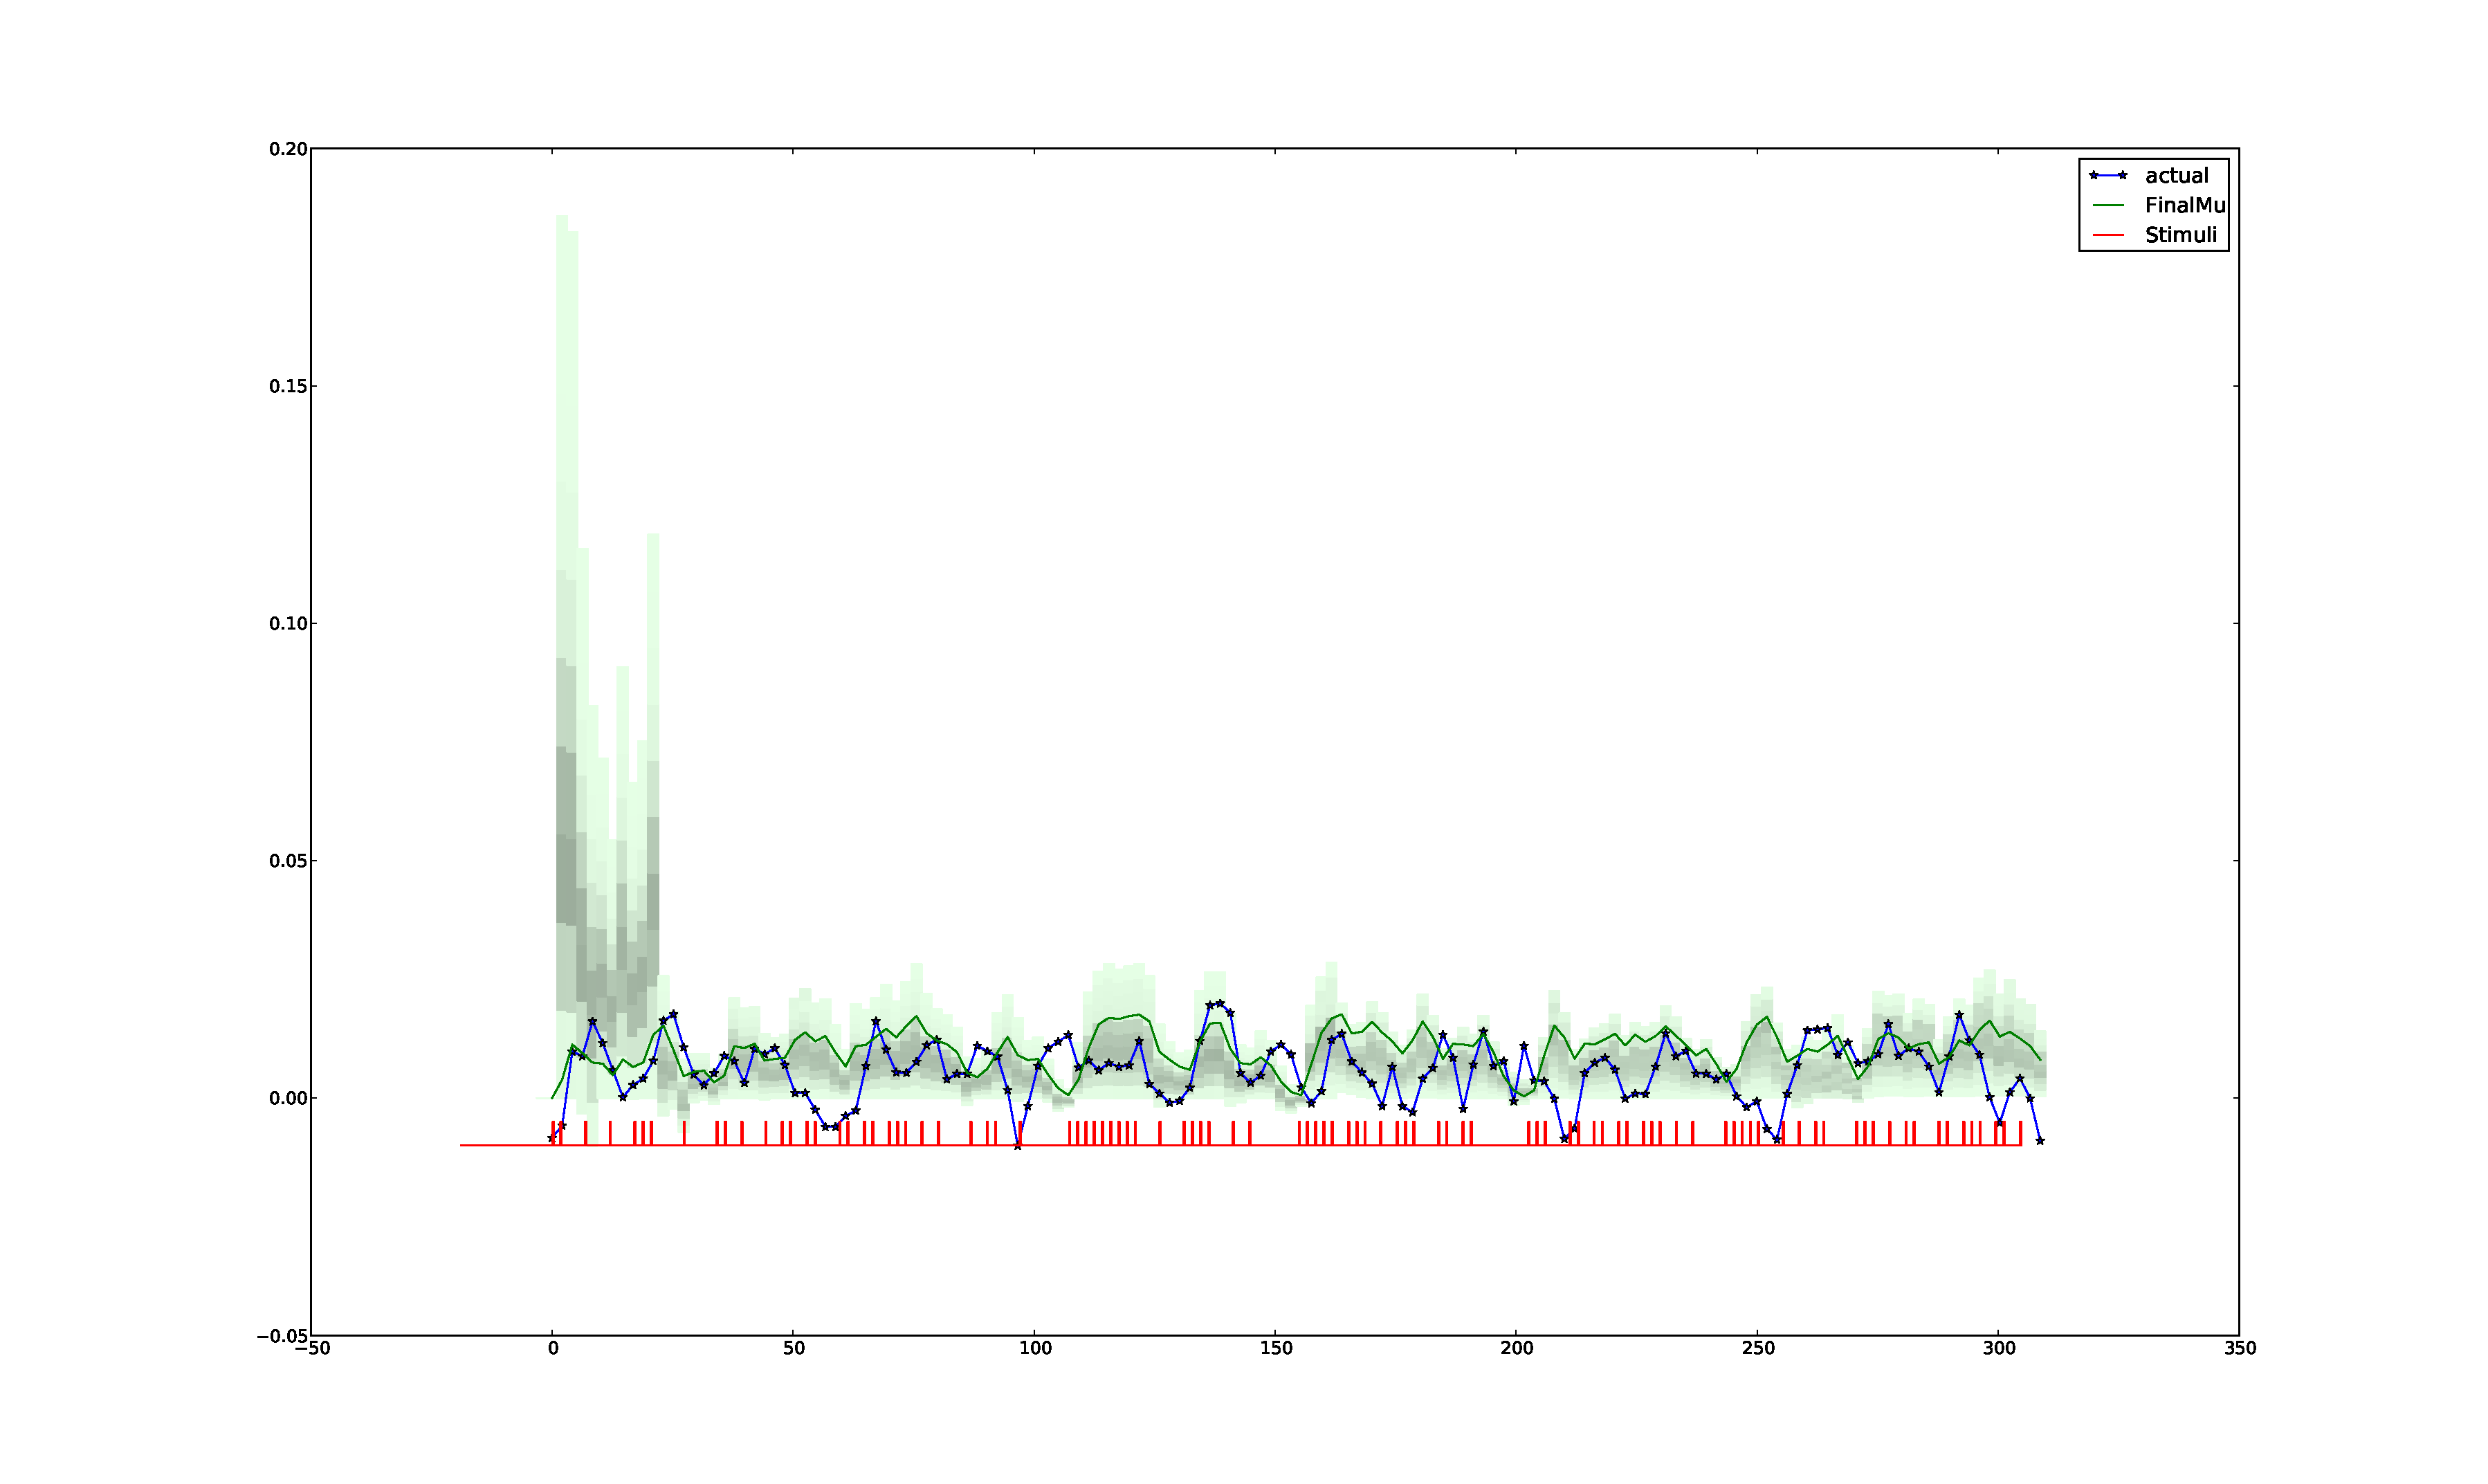
\includegraphics[clip=true,trim=6cm 2cm 6cm 3.5cm,width=17cm]{images/goodfit_param1}}
%\caption{The same priors gave rise to both fits.}
%\label{fig:badfit_param1}
%\end{figure}
%
%For this reason, I actually lowered the standard deviations of the time
%constants to prevent over-smoothing. This resulted in more consistent,
%though potentially slightly worse fits, two examples of which are 
%shown in \autoref{fig:param2_var}. 
%
%\begin{figure}
%\subfigure{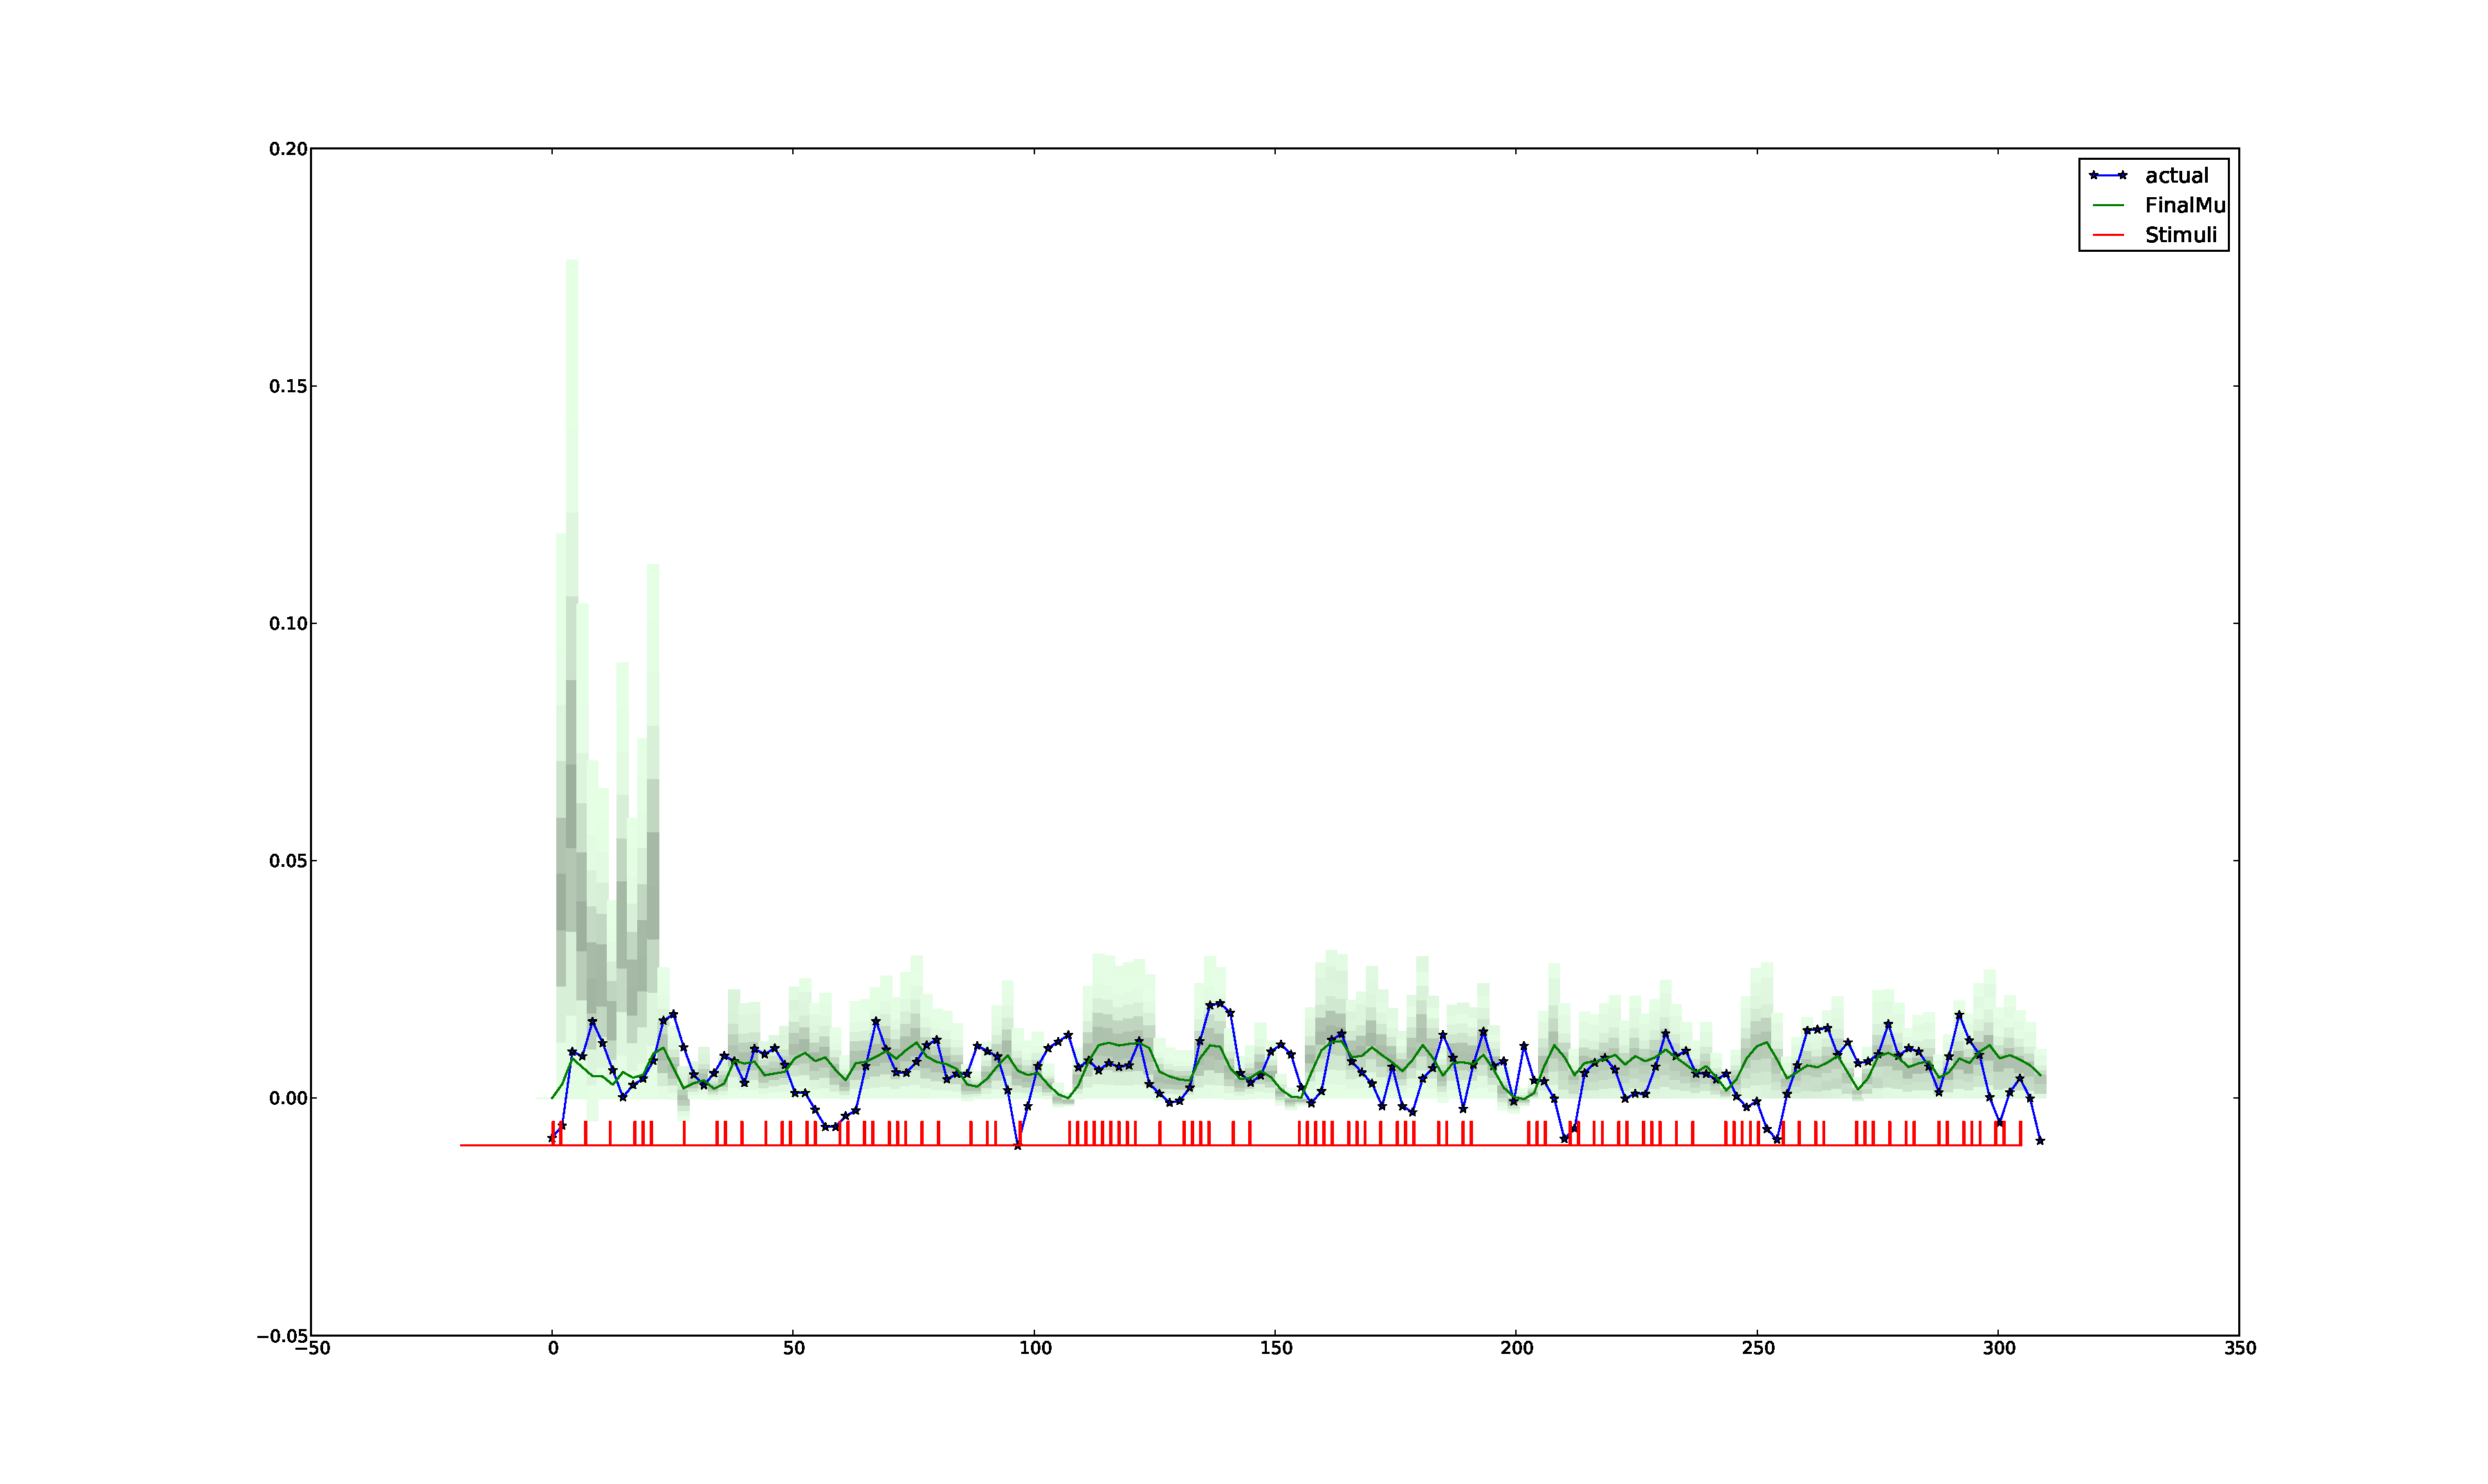
\includegraphics[clip=true,trim=6cm 2cm 6cm 3.5cm,width=17cm]{images/param2a}}
%\subfigure{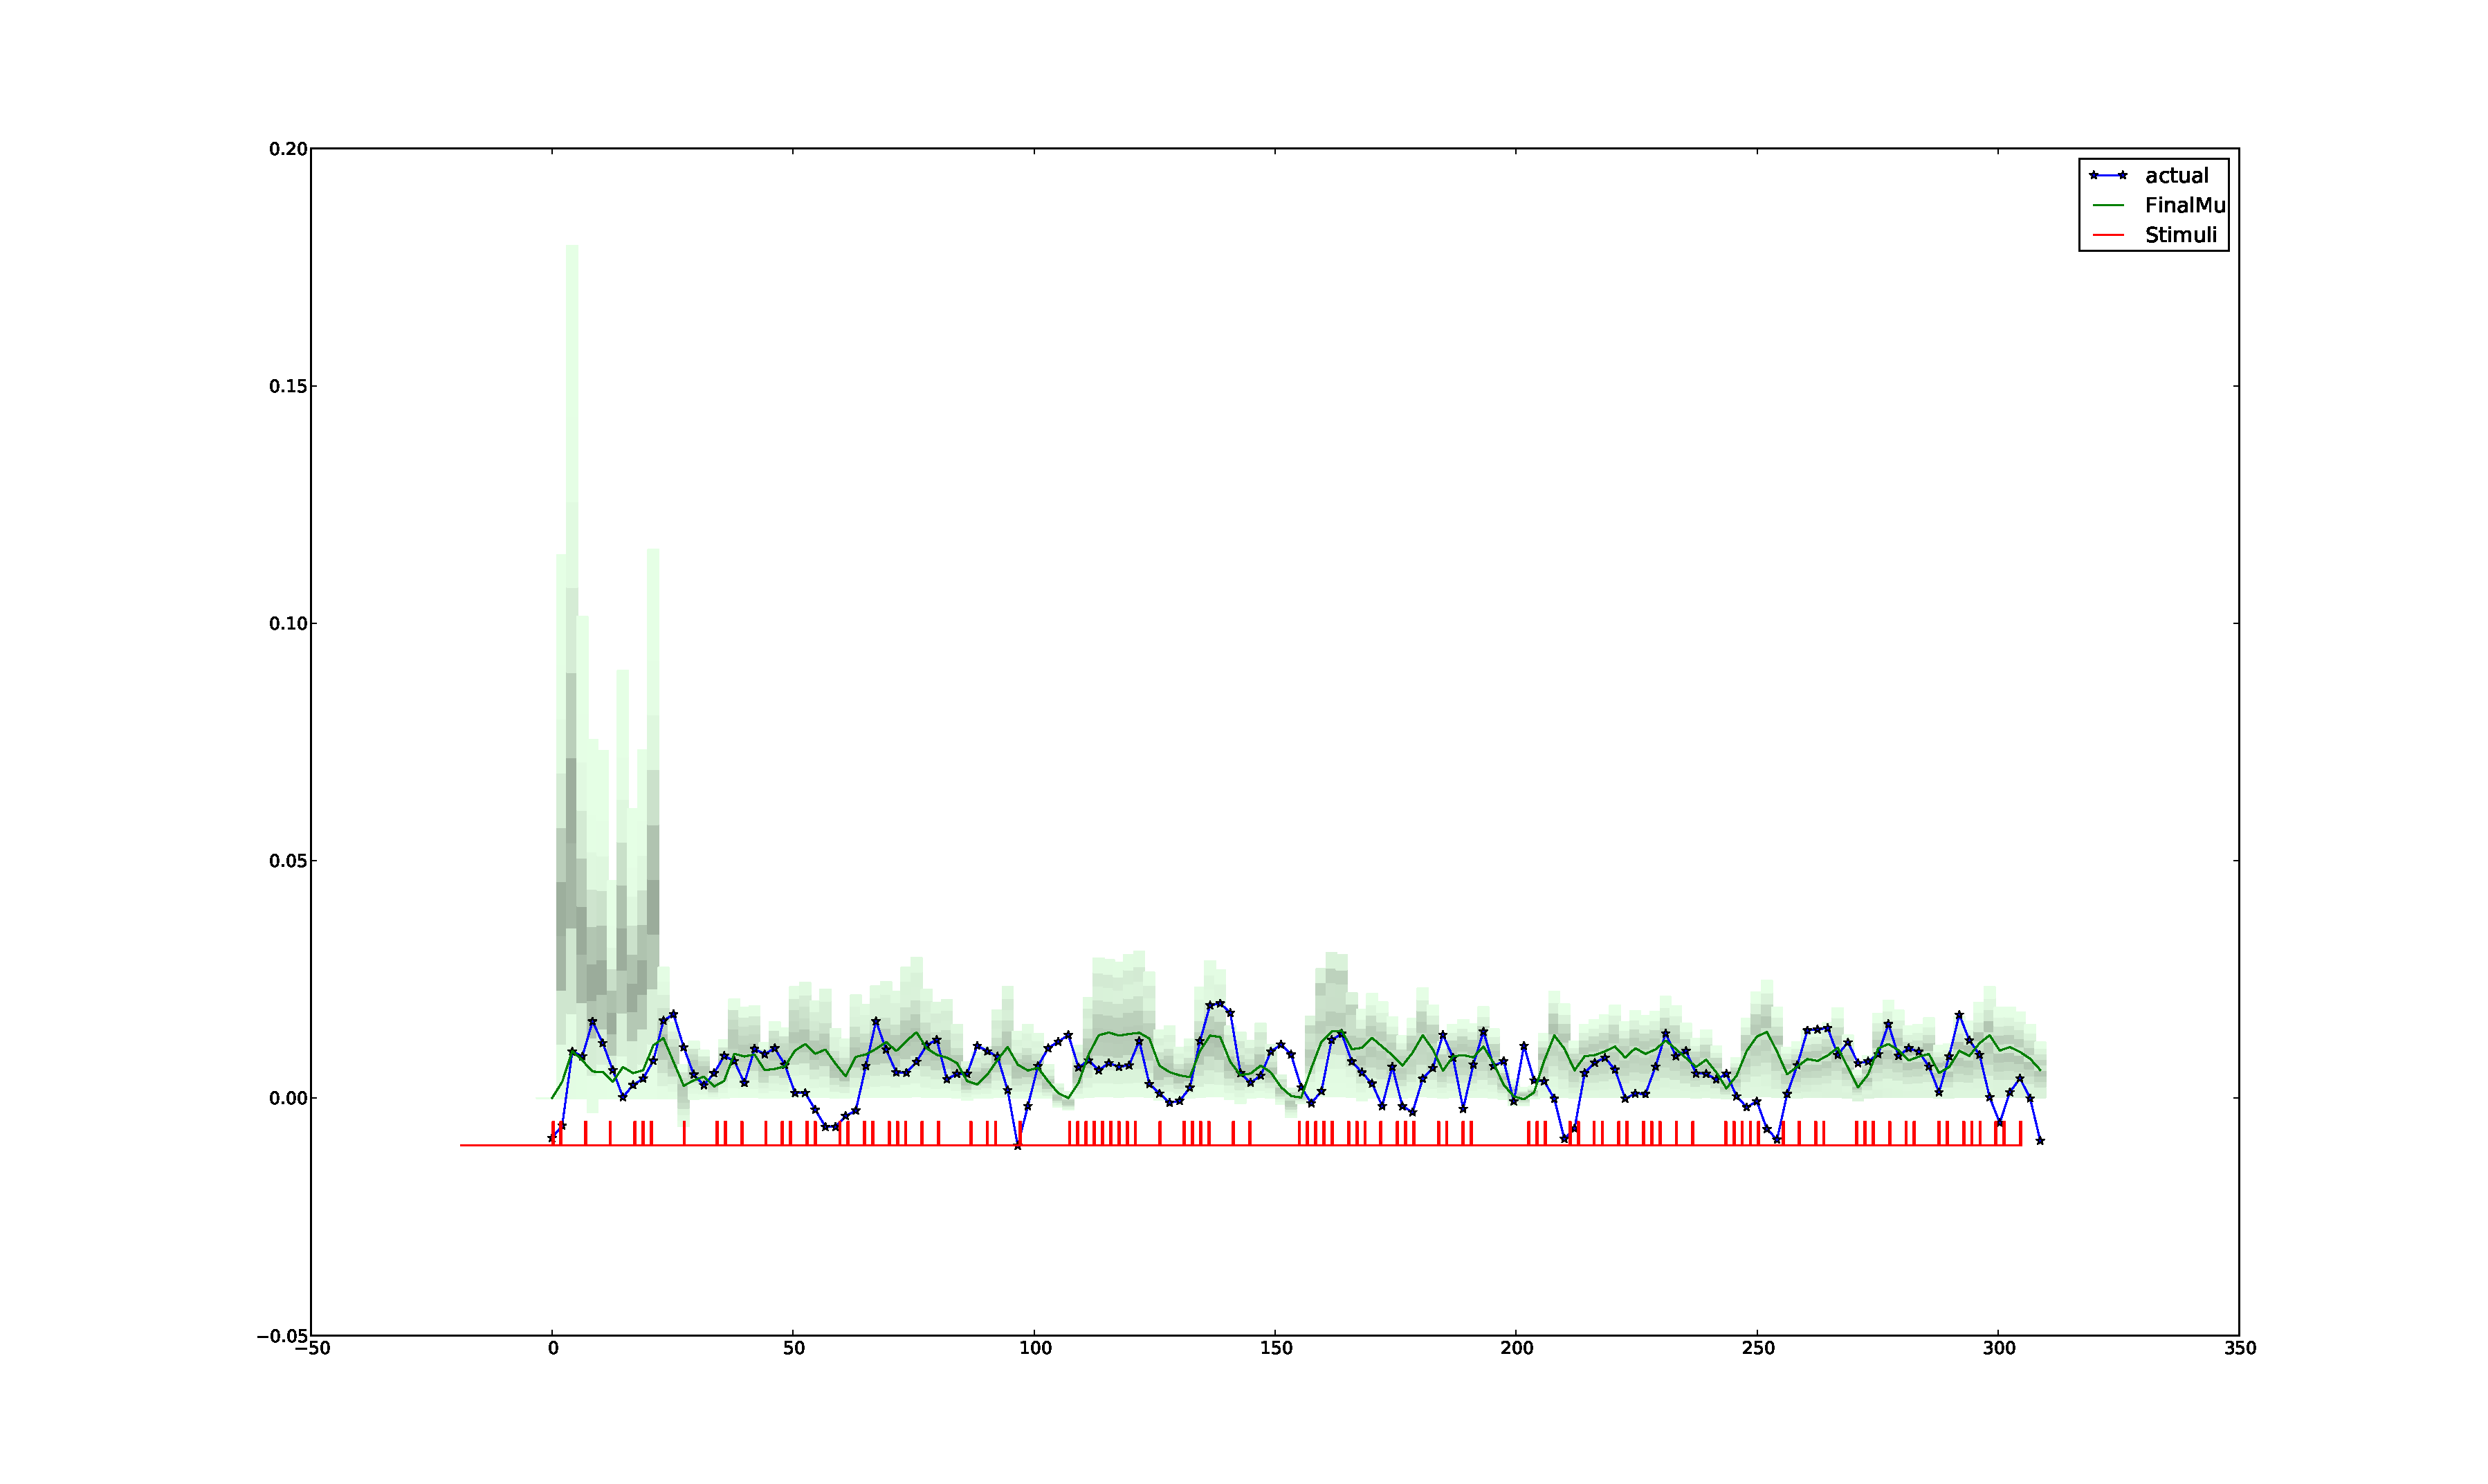
\includegraphics[clip=true,trim=6cm 2cm 6cm 3.5cm,width=17cm]{images/param2b}}
%\caption{A poor fit, using the same parameters as }
%\label{fig:param2_var}
%\end{figure}
%
%todo: stats of the 100 fits?
%
%\section{Single Time-Series Simulation}
%
\chapter{Real Data}
\label{sec:RealData}
Modeling the BOLD response is of course not of much use if does not work for
real FMRI.  Although this algorithm will hopefully lead to more novel methods 
of analysis, the standard use for modeling the BOLD signal is to locate activation.
Activation is defined as areas where the input is the primary drive
for the BOLD response, as opposed to intermediate factors controlling it. 
Once areas where the BOLD 
model may be accurately estimated are found, integrating the model will allow for accurate
estimation of the state between measurements, which could then be used for more 
advanced analysis, for instance of areas that are being driven by other brain regions.
It all begins with localizing the first activation regions in the
chain. Therefore this section compares the output of the particle filter 
with conventional SPM. 

The data described in this section are fundamentally different in several 
ways. SPM preprocesses the image by spatially smoothing the FMRI image (in this section 
SPM8 was used with an $8mm x 8mm x 8mm$ Gaussian kernel), whereas
this is not done in the particle filter algorithm. Additionally, a spline
was used to de-trend, rather than SPM8's high pass filter (with a cut
off based on a globally estimated autocorrelation). Thus the preprocessing pipelines 
are different; but the output of SPM8 is also different. Whereas SPM outputs
a t-statistic for each voxel, the output 
of the particle filter is a posterior probability distribution of the parameters
at every voxel. To validate the quality of the particle filter results 
it is necessary to compare the both the location and the fit calculated by the particle filter
with SPM's location and fit.

\section{Results}
The results from T-values from SPM8 are shown in \autoref{fig:hm_canon_spm} (threshold of
4), and the results from 
the particle filter are shown in \autoref{fig:hm_canon_pfilter} and \autoref{fig:hm_canon_pfilter_mi}.
Note that the scales for all three images are different, because the metrics are different.
SPM measures using T-Tests to determine the likelihood of a false positive. \autoref{fig:hm_canon_pfilter}
uses simple normalized residuals, meaning that lower indicates less error.  
\autoref{fig:hm_canon_pfilter_mi} measures in terms of the dependence between the 
measured signal and the estimated signal; thus higher indicates a better fit. The particle
filter data shows a large number of false positives, however application of a threshold
of $.85$ on the residual map removes these false positives. Similarly, in the mutual information
map, the false positives may be elminated by upping the threshold to $.15$. However, just
because the results disagree with SPM does not necessarily mean they are false positives.
SPM operates on smoothed data (8mm x 8mm x 8mm), so there are certainly active 
areas that have been missed because of the smoothing. 

\begin{figure}[H]
\subfigure[]{\label{fig:hm_spm} 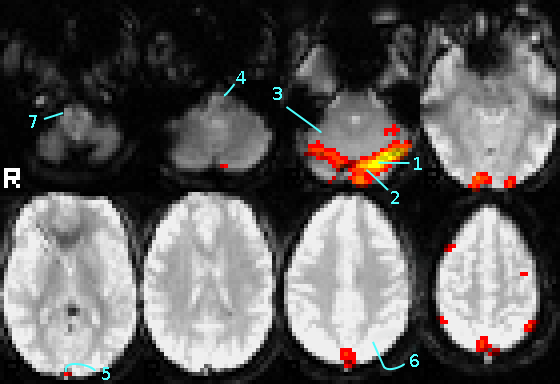
\includegraphics[scale=.85]{images/spm_hm}}
\subfigure[]{\label{fig:hm_canon_spm_x} 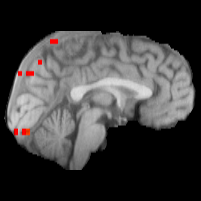
\includegraphics[scale=3]{images/spm_hm_x}}
\subfigure[]{\label{fig:hm_canon_spm_y} 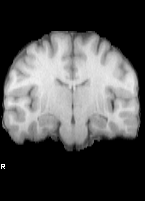
\includegraphics[scale=3]{images/spm_hm_y}}
\subfigure[]{\label{fig:hm_canon_spm_z} 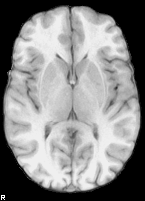
\includegraphics[scale=3]{images/spm_hm_z}}
\subfigure{\label{fig:scale_spm} 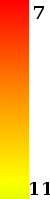
\includegraphics[scale=.5]{images/scale1}}
\caption{Sagittal, coronal and axial slices of SPM results (\autoref{fig:hm_canon_spm_x} \autoref{fig:hm_canon_spm_y} 
         \autoref{fig:hm_canon_spm_x}), as well as a series of axial slices, \autoref{fig:hm_spm}. Units
         of activation are in Student's T-scores. Higher indicates higher assurance that the signal cannot
         have occurred through noise alone.}
\label{fig:hm_canon_spm}
\end{figure}

\begin{figure}[H]
\subfigure[]{\label{fig:hm_pfilter} 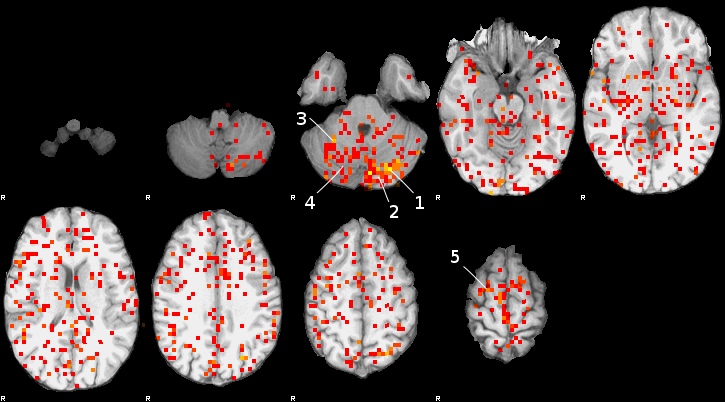
\includegraphics[scale=.85]{images/pfilter_hm}}
\subfigure[]{\label{fig:hm_canon_pfilter_x} 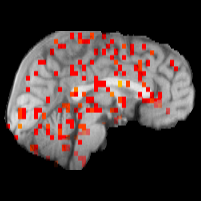
\includegraphics[scale=3]{images/pfilter_hm_x}}
\subfigure[]{\label{fig:hm_canon_pfilter_y} 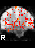
\includegraphics[scale=3]{images/pfilter_hm_y}}
\subfigure[]{\label{fig:hm_canon_pfilter_z} 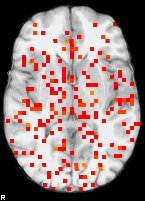
\includegraphics[scale=3]{images/pfilter_hm_z}}
\subfigure{\label{fig:scale_pfilter} 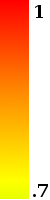
\includegraphics[scale=.5]{images/scale2}}
\caption{Sagittal, coronal and axial (\autoref{fig:hm_canon_pfilter_x} \autoref{fig:hm_canon_pfilter_y} 
         \autoref{fig:hm_canon_pfilter_x}), as well as a series of axial slices, \autoref{fig:hm_pfilter}. 
         Units of match is normalized residual. The lowest (best) levels were $.7$.
         The highest error shown is $1$.}
\label{fig:hm_canon_pfilter}
\end{figure}

%\begin{figure}[H]
%\subfigure[]{\label{fig:hm_pfilter85} 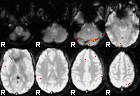
\includegraphics[scale=.75]{images/pfilter85_hm}}
%\subfigure[]{\label{fig:hm_canon_pfilter85_x} 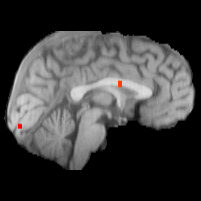
\includegraphics[scale=3]{images/pfilter_hm85_x}}
%\subfigure[]{\label{fig:hm_canon_pfilter85_y} 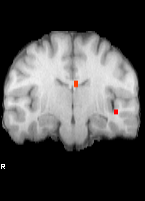
\includegraphics[scale=3]{images/pfilter_hm85_y}}
%\subfigure[]{\label{fig:hm_canon_pfilter85_z} 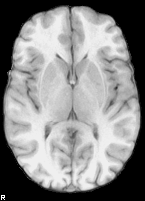
\includegraphics[scale=3]{images/pfilter_hm85_z}}
%\subfigure{\label{fig:scale_pfilter85} 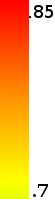
\includegraphics[scale=.5]{images/scale3}}
%\caption{Sagittal, coronal and axial (\autoref{fig:hm_canon_pfilter_x} \autoref{fig:hm_canon_pfilter_y} 
%         \autoref{fig:hm_canon_pfilter_x}), as well as a series of axial slices, \autoref{fig:hm_pfilter}. 
%         Units of match is normalized residual. The lowest (best) levels were $.7$.
%         The highest error shown is $.85$.}
%\label{fig:hm_canon_pfilter85}
%\end{figure}

\begin{figure}[H]
\subfigure[]{\label{fig:hm_mi} 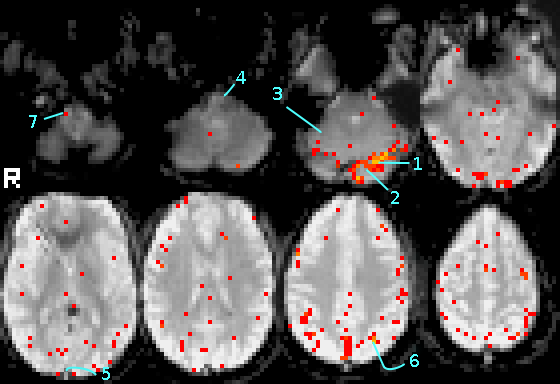
\includegraphics[scale=.85]{images/mi_hm}}
\subfigure[]{\label{fig:hm_canon_mi_x} 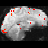
\includegraphics[scale=3]{images/mi_hm_x}}
\subfigure[]{\label{fig:hm_canon_mi_y} 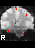
\includegraphics[scale=3]{images/mi_hm_y}}
\subfigure[]{\label{fig:hm_canon_mi_z} 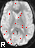
\includegraphics[scale=3]{images/mi_hm_z}}
\subfigure{\label{fig:scale_mi} 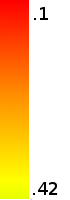
\includegraphics[scale=.5]{images/scale4}}
\caption{Sagittal, coronal and axial (\autoref{fig:hm_canon_pfilter_x} \autoref{fig:hm_canon_pfilter_y} 
         \autoref{fig:hm_canon_pfilter_x}), as well as a series of axial slices, \autoref{fig:hm_pfilter}. 
         Units of match is bits (standard for base-2 Mutual Information). The highest (best) levels are 
         $.42$. The worst shown is $.1$.}
\label{fig:hm_canon_pfilter_mi}
\end{figure}

\begin{figure}
\subfigure[Particle Filter]{\label{fig:comp1pfilter} 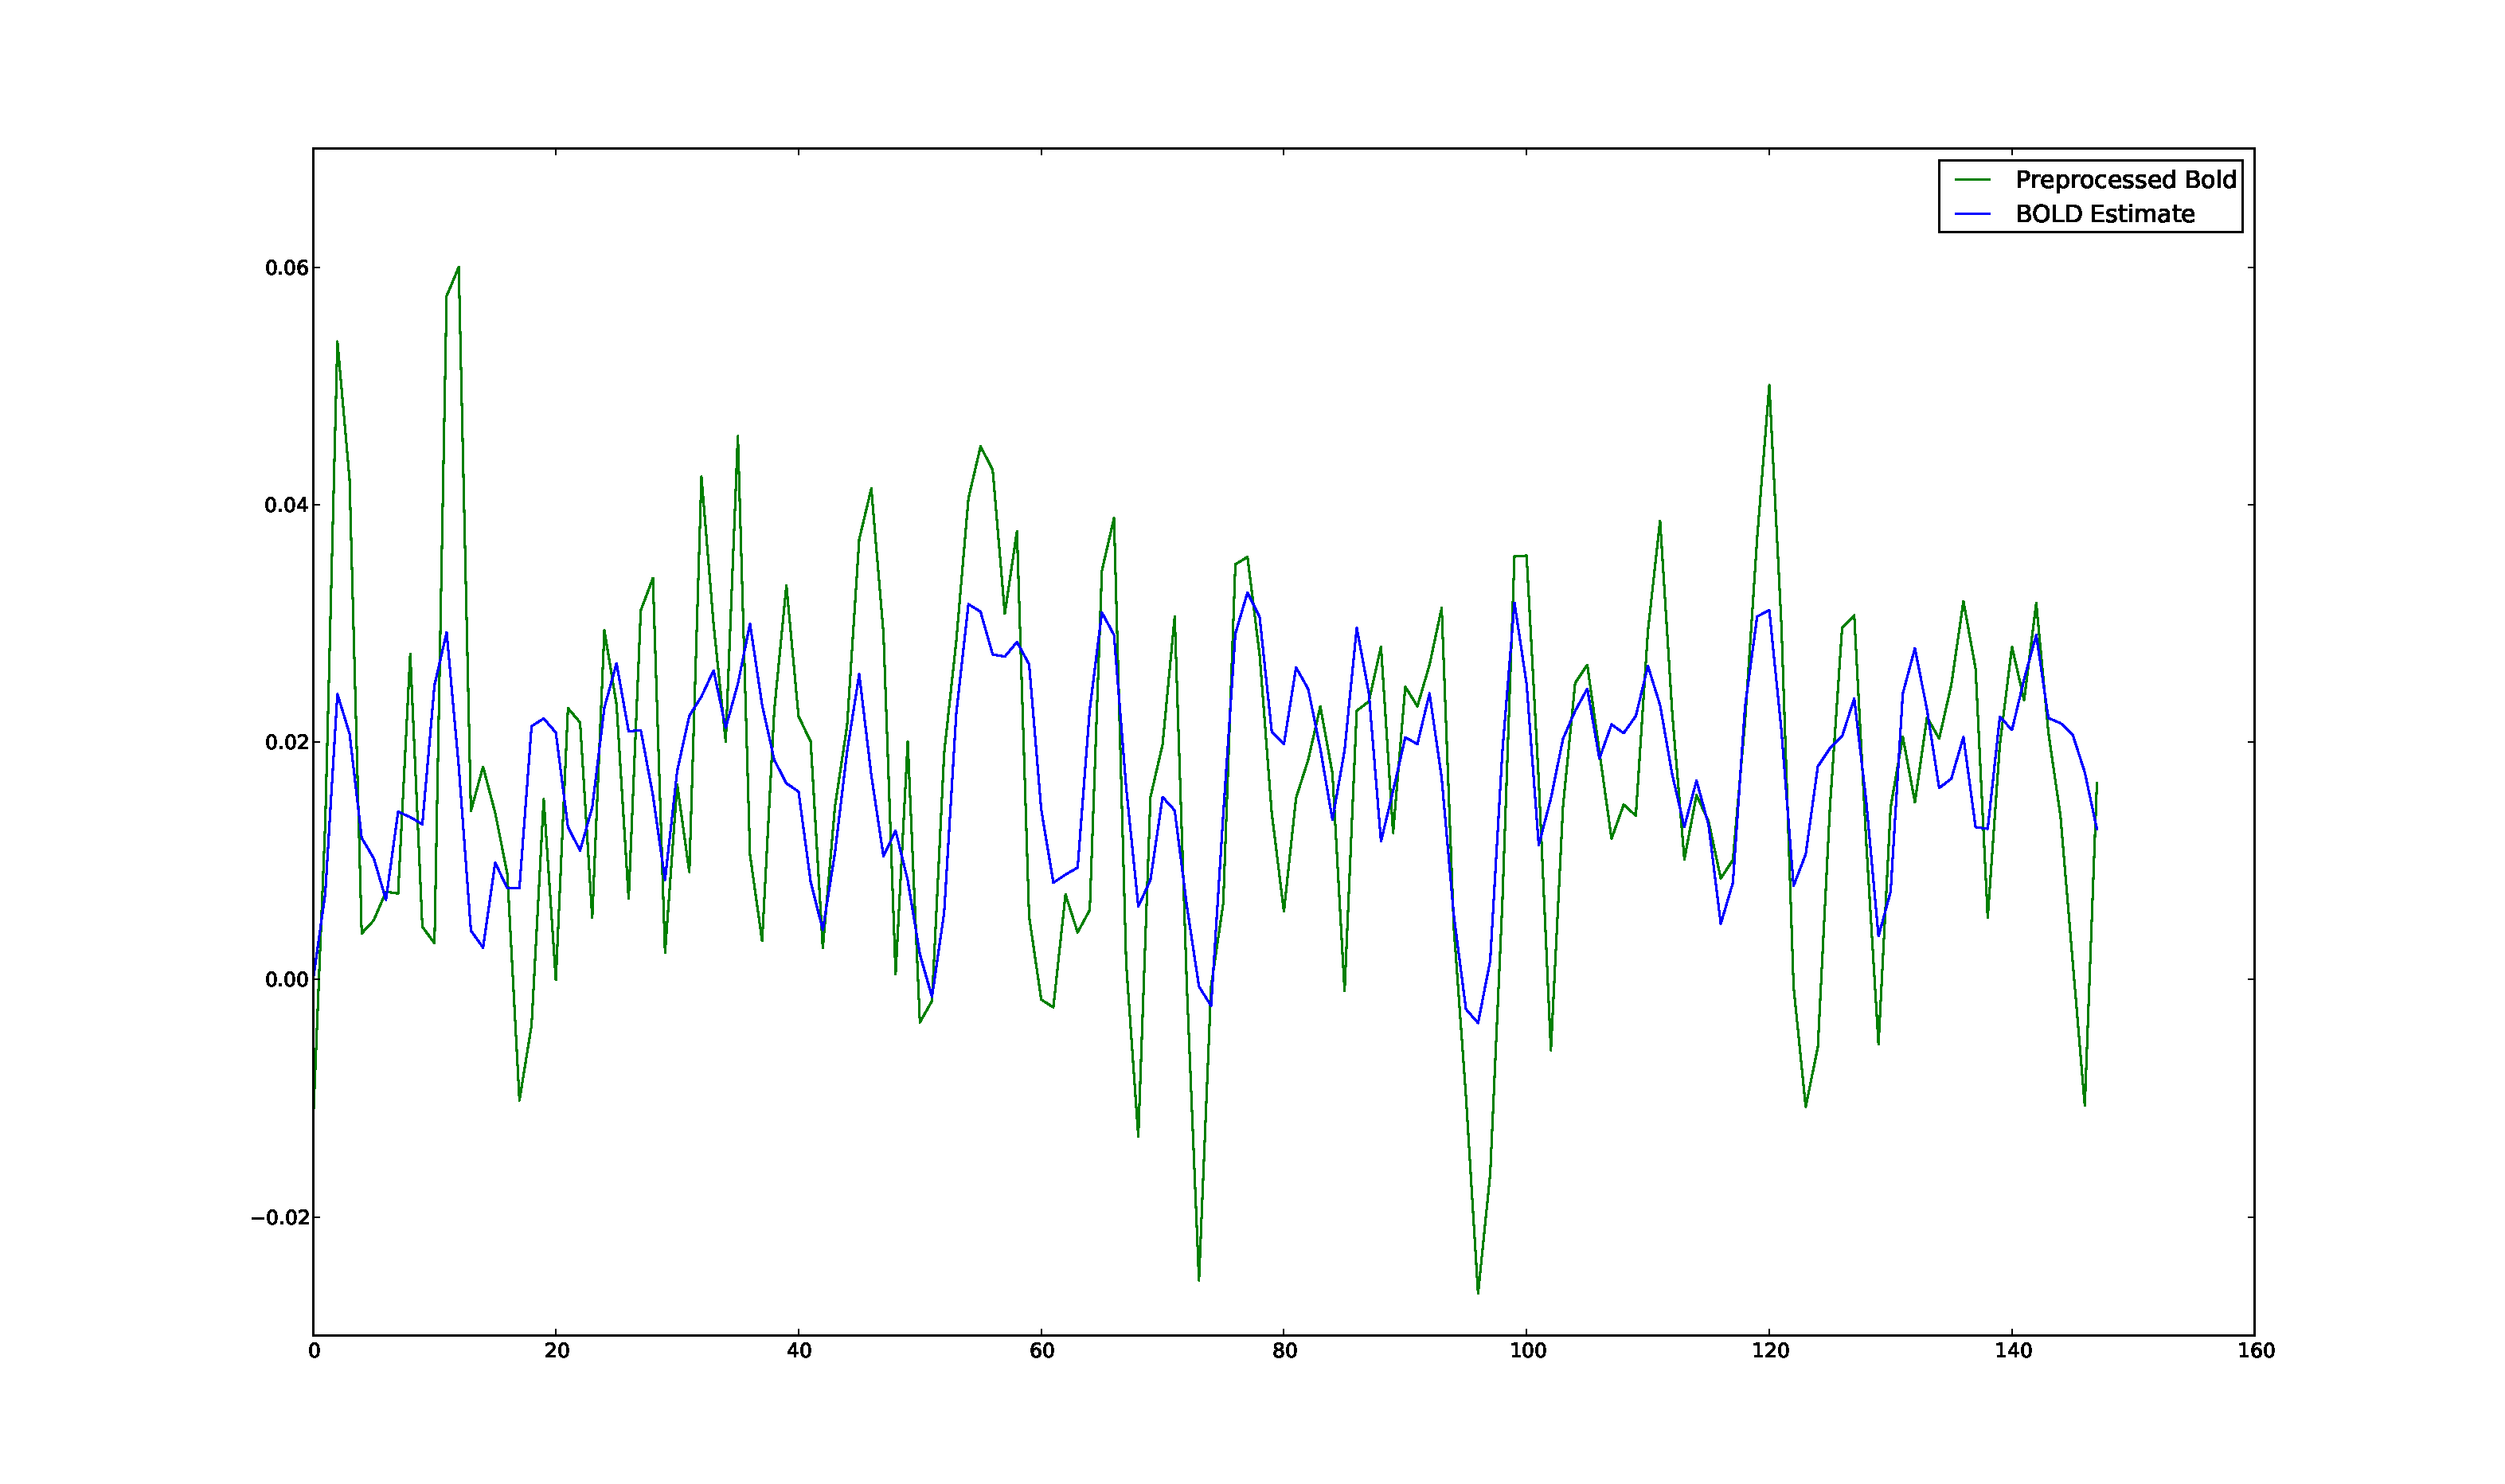
\includegraphics[clip=true,trim=5cm 1cm 4cm 1cm,width=15cm]{images/1_pfilter_37_14_7}}\\
\subfigure[SPM]{\label{fig:comp1spm} 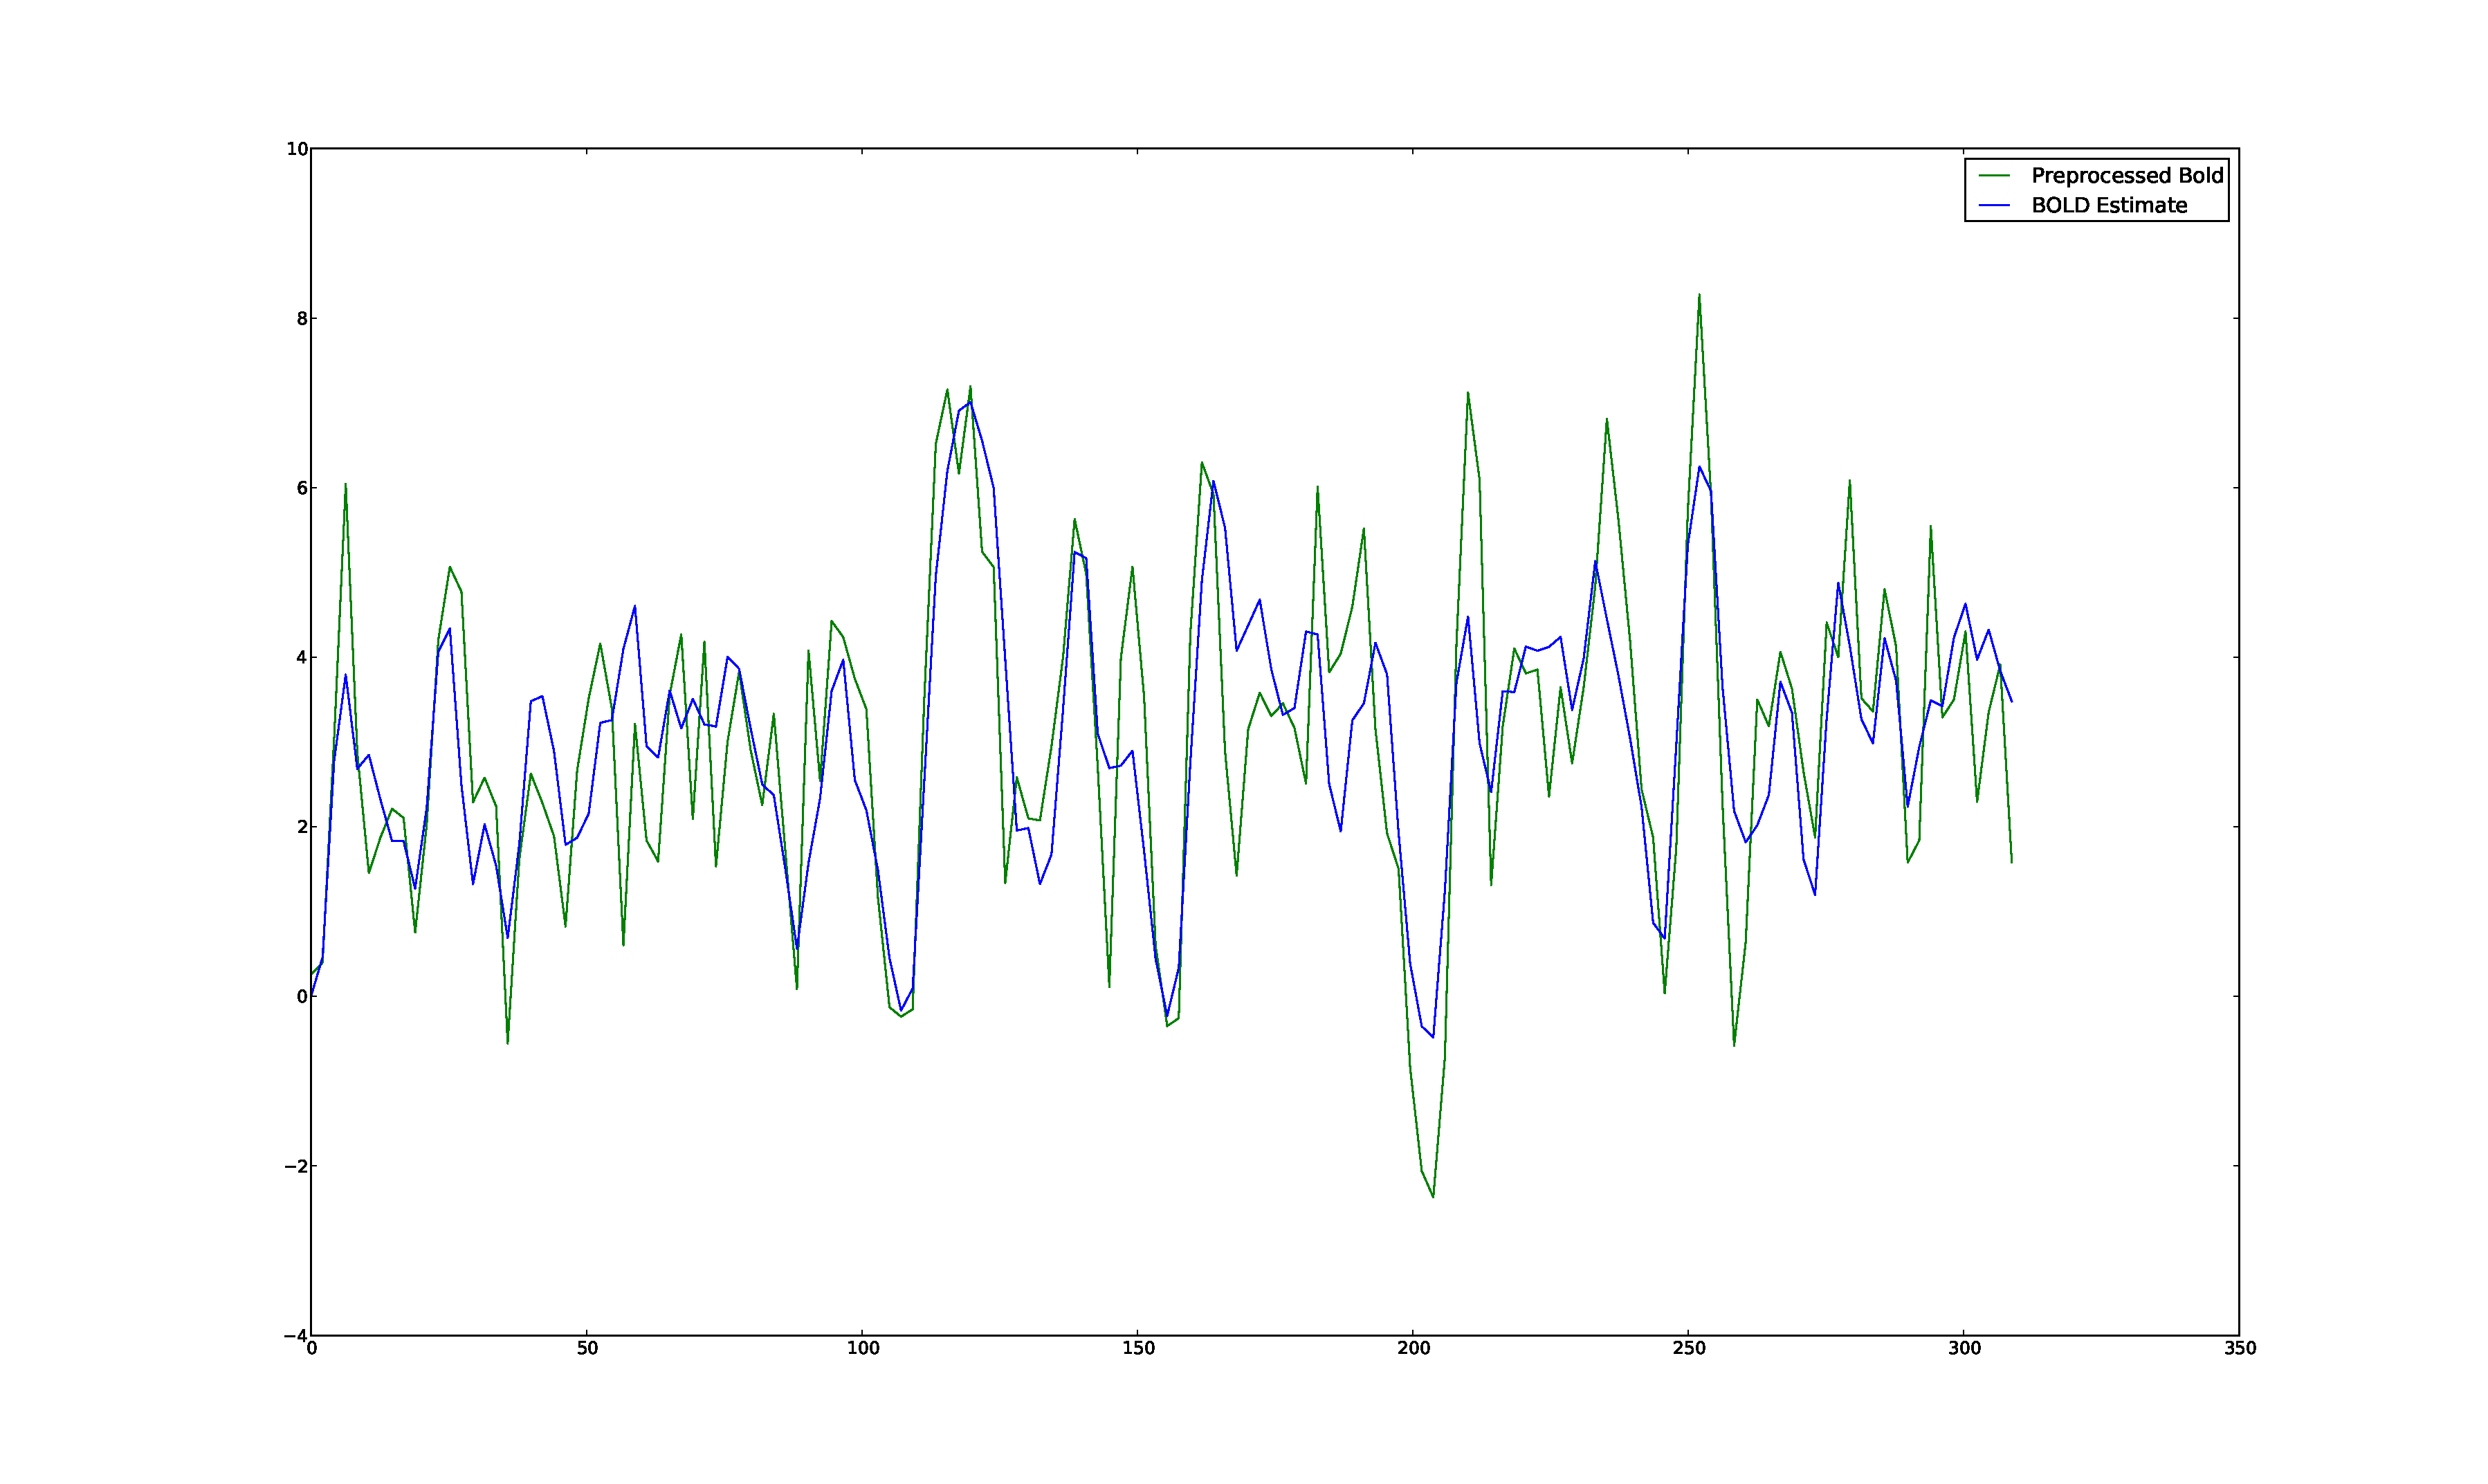
\includegraphics[clip=true,trim=5cm 1cm 4cm 1cm,width=15cm]{images/1_spm_37_14_7}}
\caption{Section 1, Estimated vs. Actual BOLD response}
\label{fig:comp1}
\end{figure}

 
\begin{figure}
\subfigure[Particle Filter]{\label{fig:comp2pfilter} 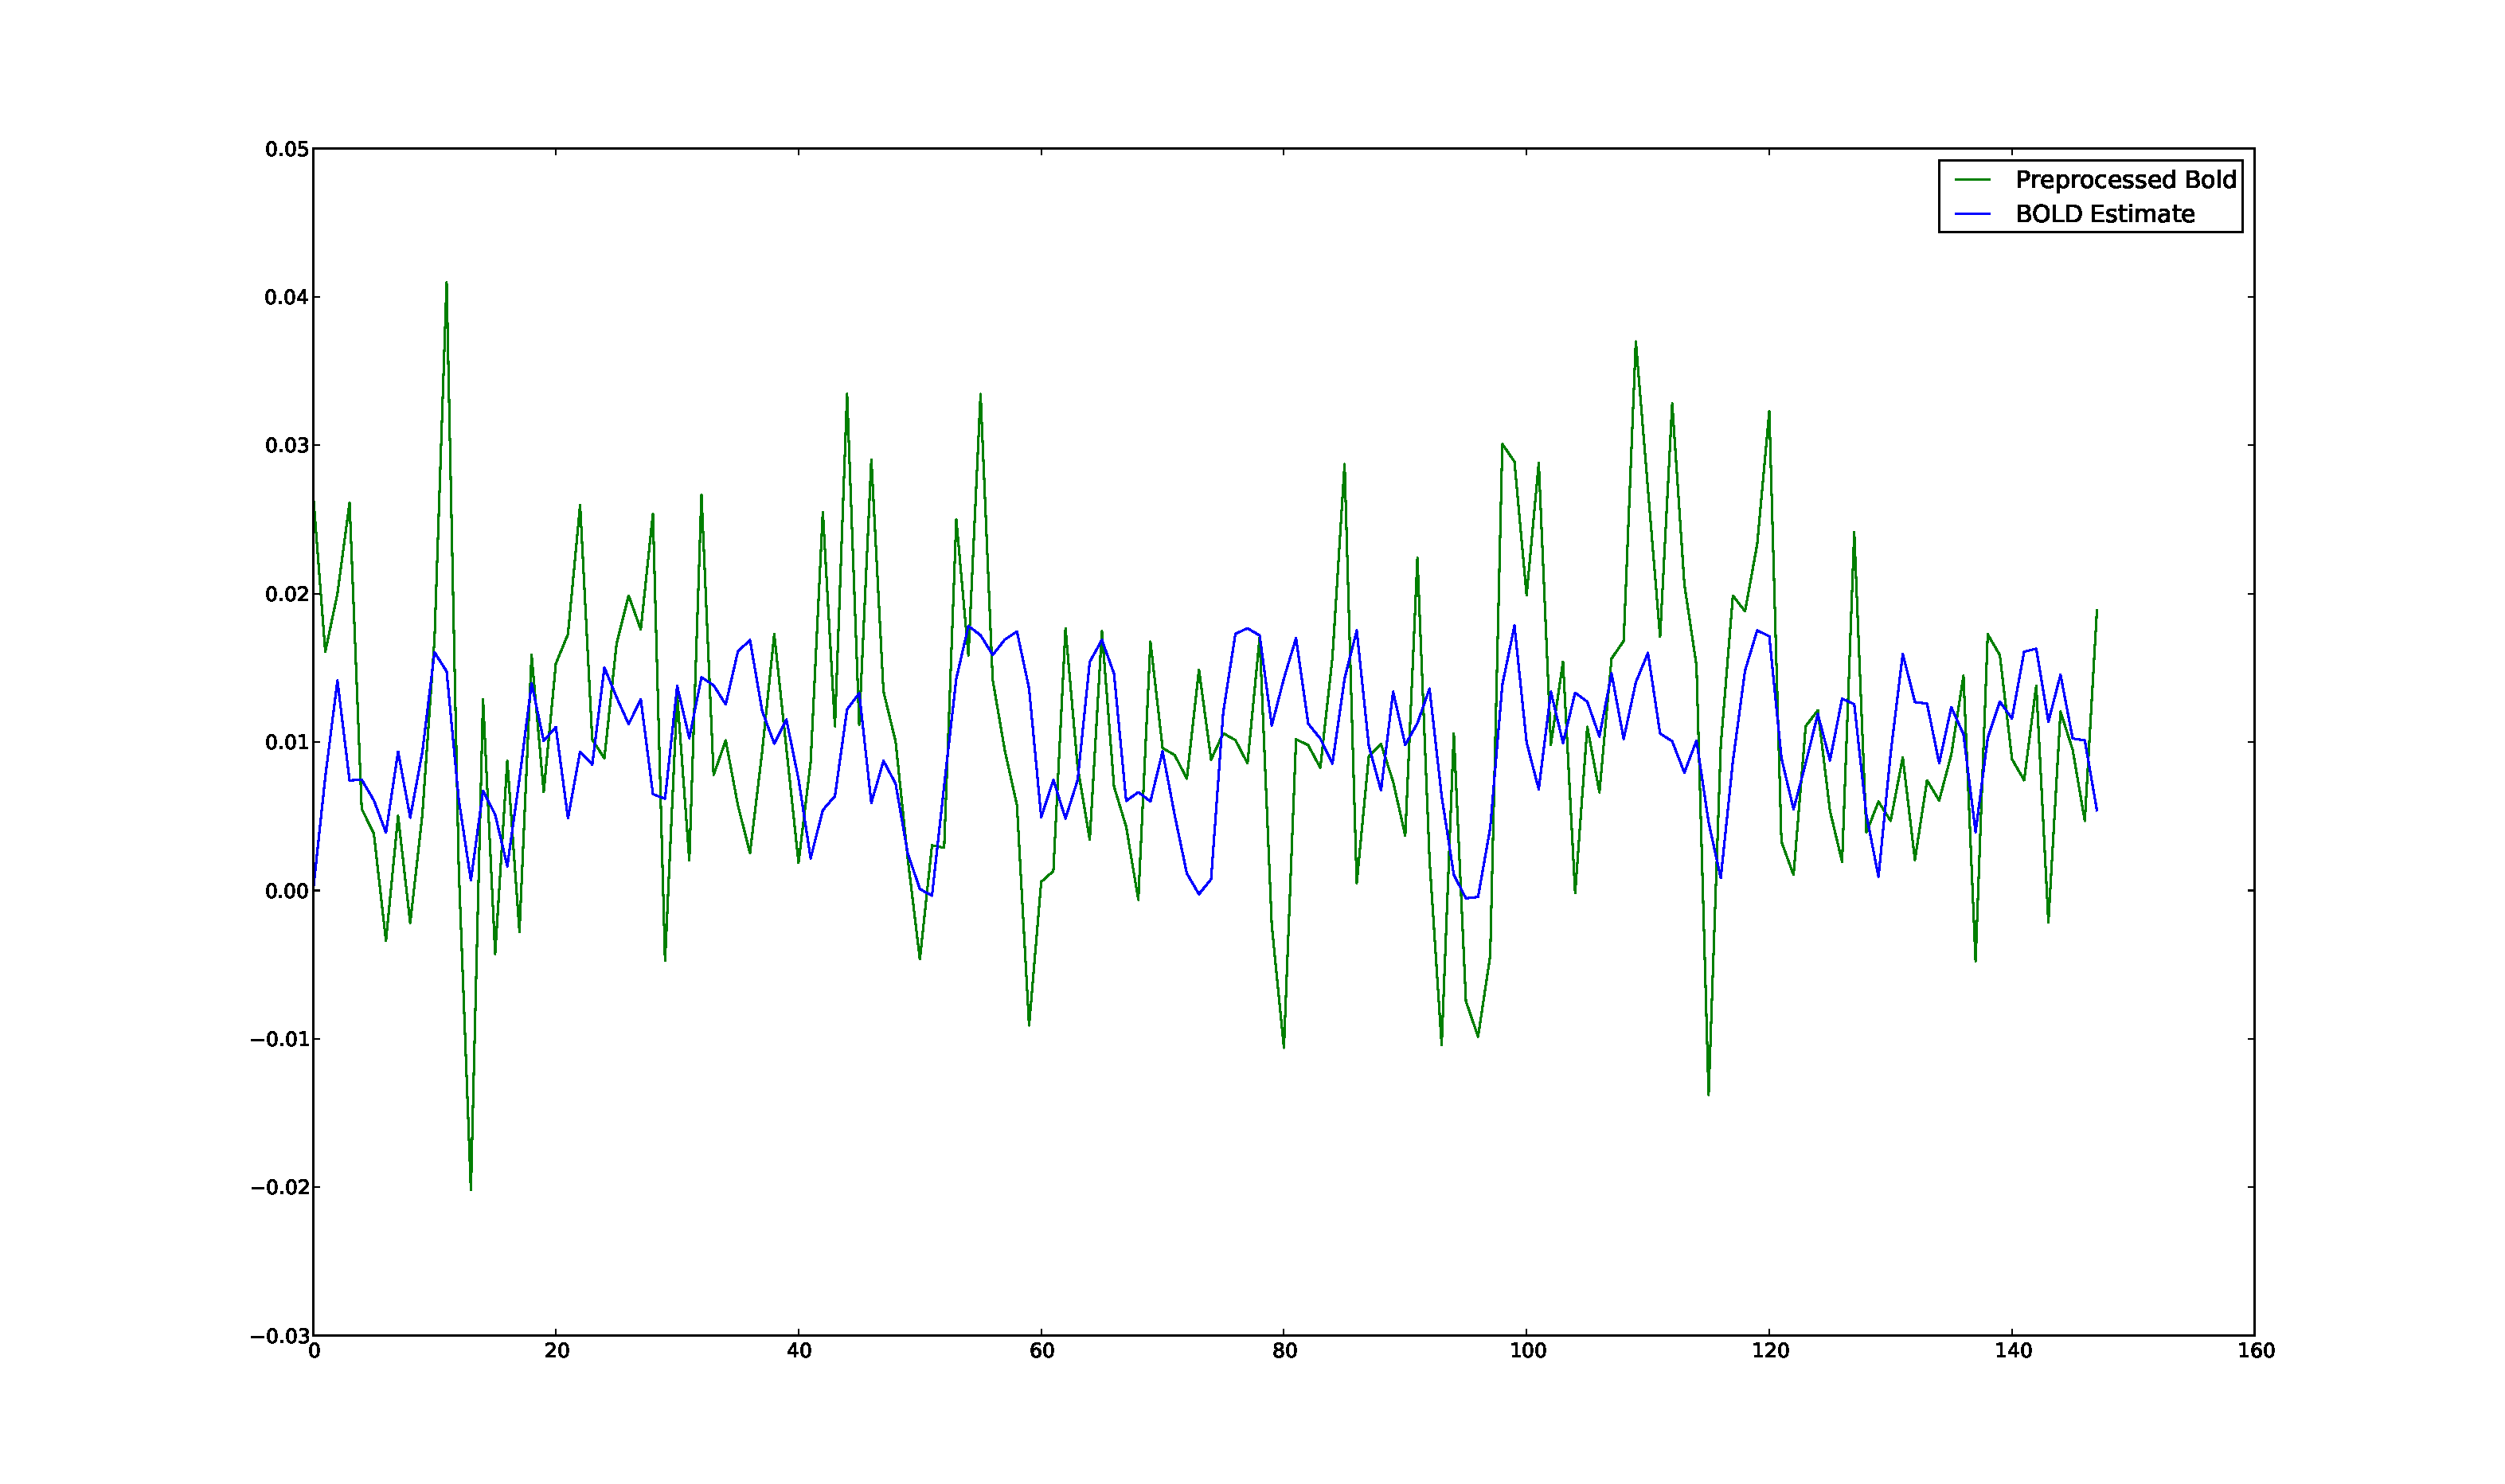
\includegraphics[clip=true,trim=5cm 1cm 4cm 1cm,width=15cm]{images/2_pfilter_34_12_7}}\\
\subfigure[SPM]{\label{fig:comp2spm} 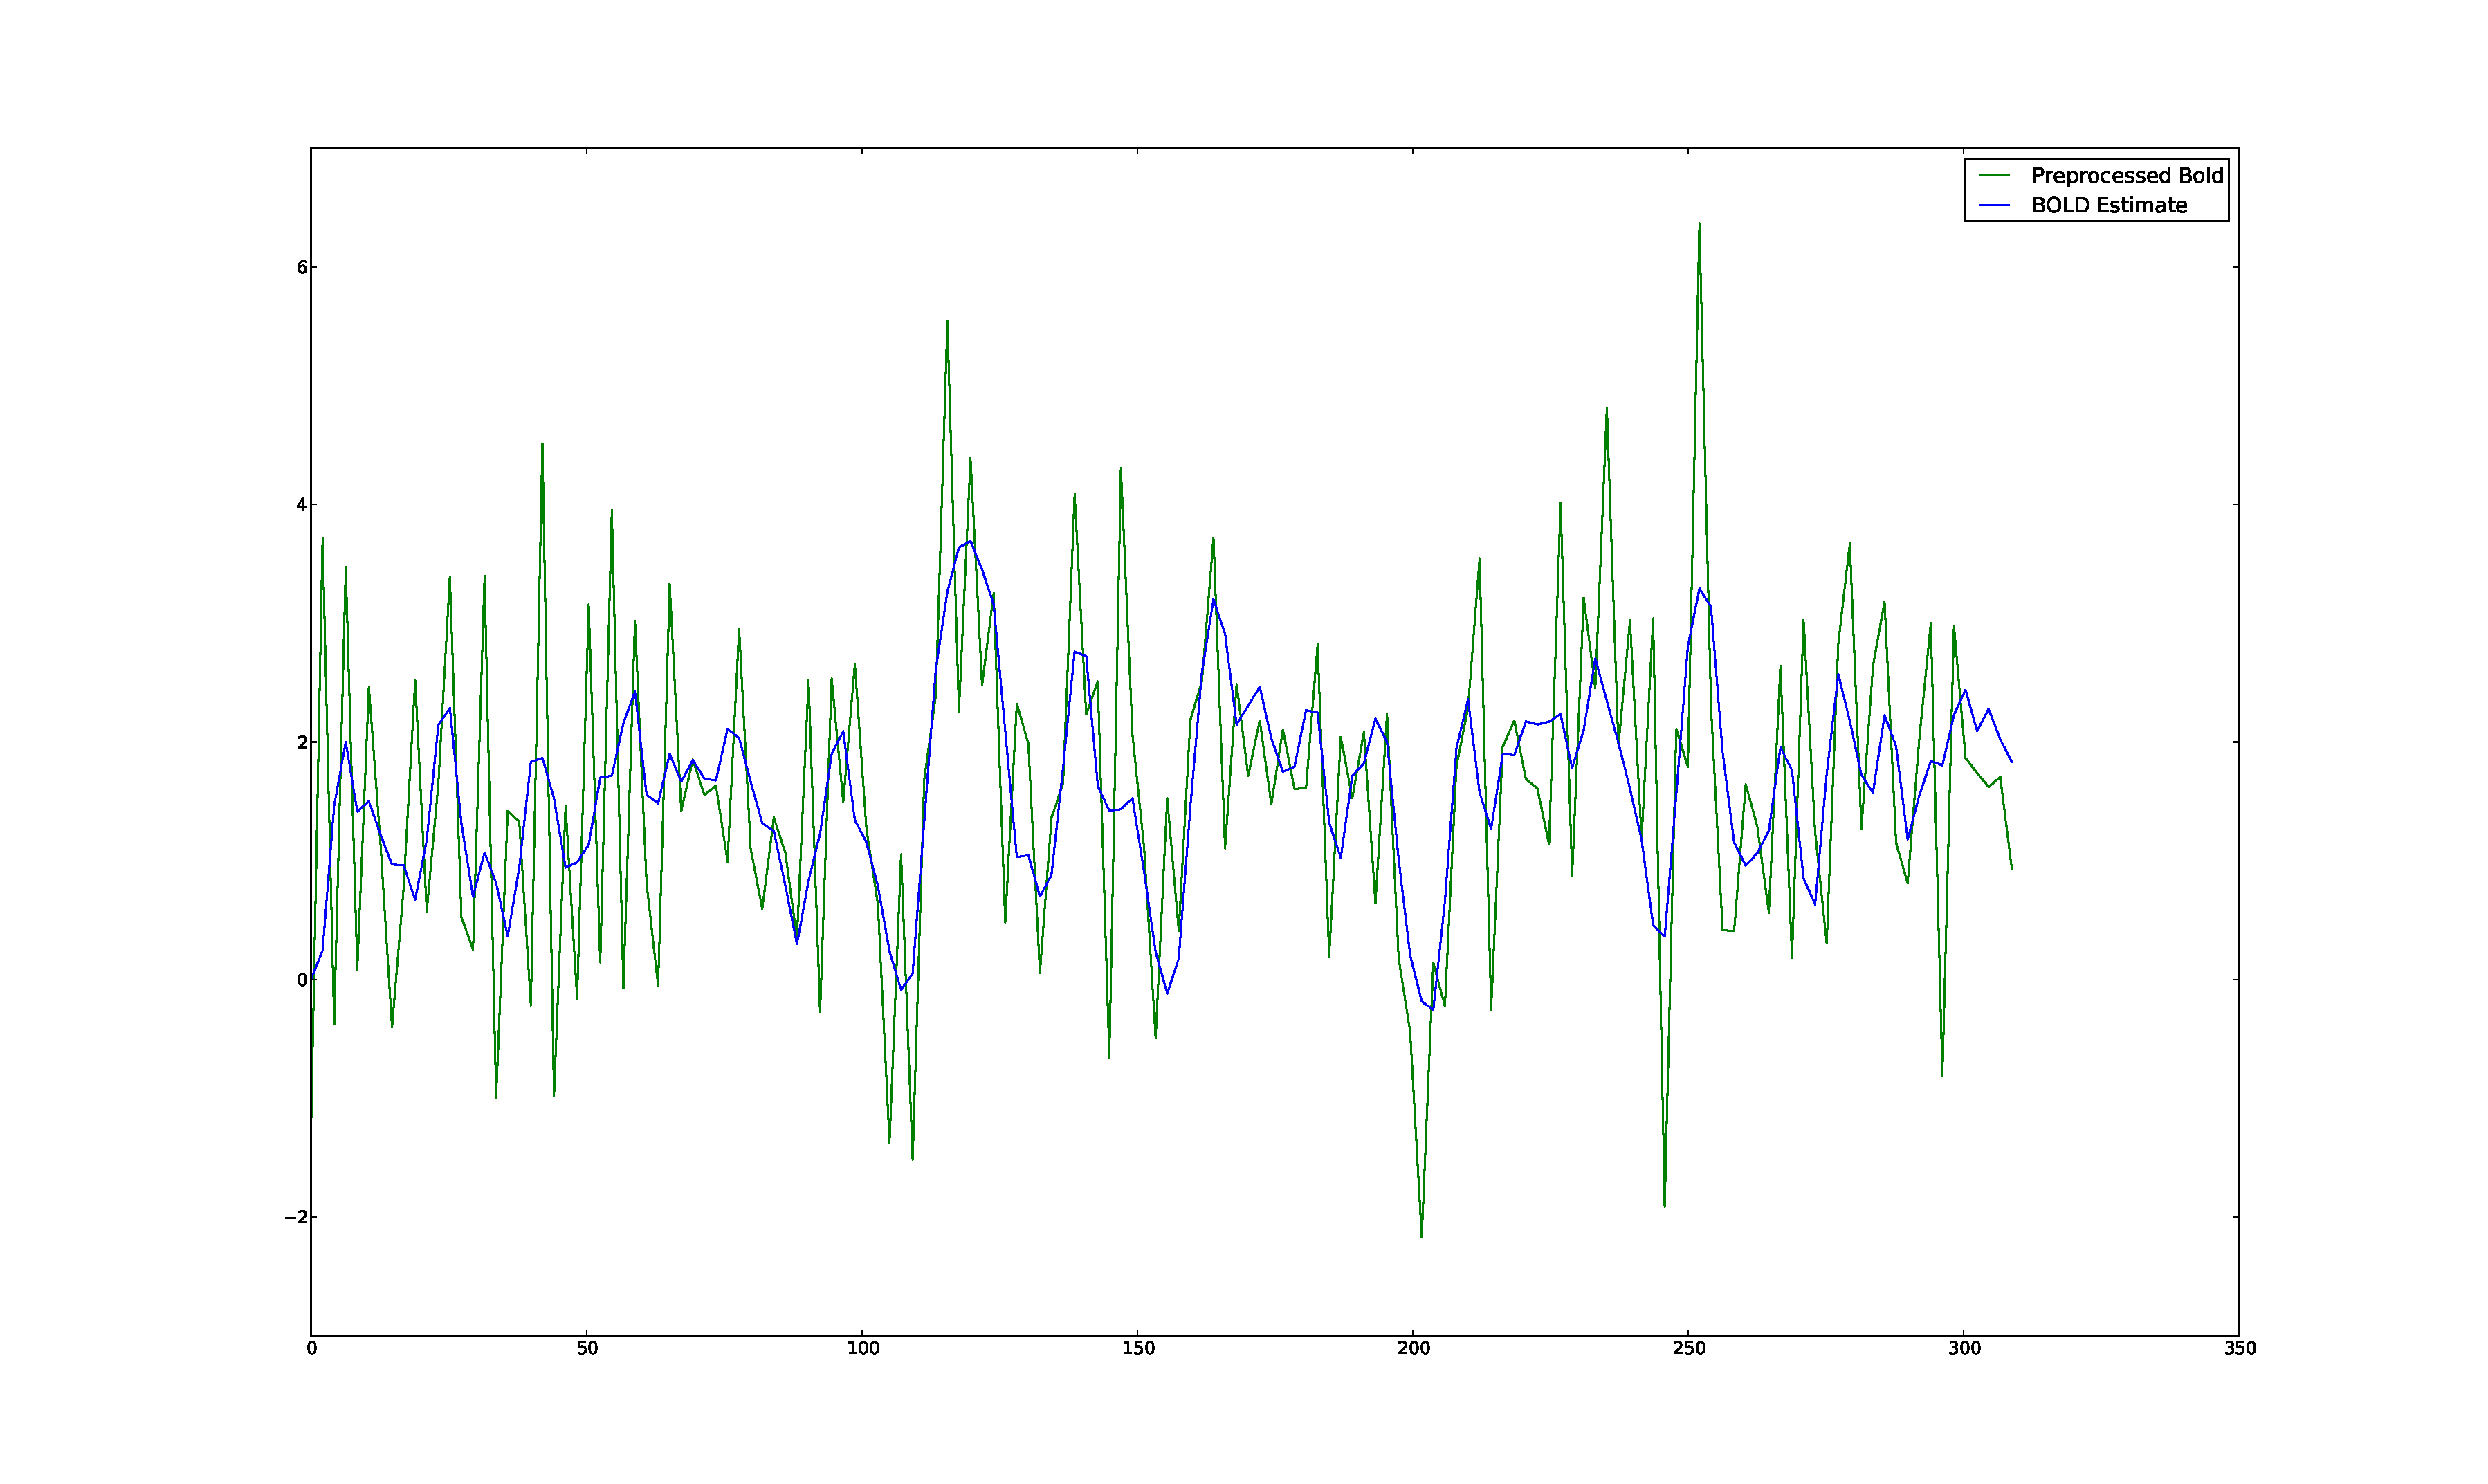
\includegraphics[clip=true,trim=5cm 1cm 4cm 1cm,width=15cm]{images/2_spm_34_12_7}}
\caption{Section 2, Estimated vs. Actual BOLD response}
\label{fig:comp2}
\end{figure}

I chose several voxels to discuss further from \autoref{fig:hm_canon_pfilter} and \autoref{fig:hm_canon_spm}.
The first voxel, labeled 1, had a very high T-score, high mutual information,  as well as 
a low error (around $.7$). Thus, the
fit should be very good in both the SPM and particle filter output; this comparison is shown in 
\autoref{fig:comp1}. Recall that SPM worked on a slightly less noisy time series because of the
spatial smoothing; this explains the lack of the sharp peak in the particle filter's preprocessed
data. Regardless, as expected, both work. 

I chose the second voxel (\autoref{fig:comp2}) because it was active in SPM and it would appear to be in a prime
location to be active in the SPM image (given the results in the surrounding voxels). The fit,
however shows just why the residual was high and the mutual information was low. This is a
prime example of a false positive due to the large smoothing kernel applied by SPM. 
For instance at 75 seconds, the stimulus is not present, and so the signal should drop off; yet
it doesn't. While a few peaks seem to match, most of the signal does not correlate with the
expected state progression. This voxel is not being driven direcly by the input, although it
may be gated or driven through intermediate region. 

The third voxel, compared in \autoref{fig:comp3}, was far away from any other active voxels 
and yet had a very low (around $.7$) residual. At the same time, the mutual information was
high enough to make the point suspect. Although the estimated signal seems to run down the
middle of the measurement signal; it is clear that there is a significant amount of noise
present in the signal that is not being explained by the particle filter, 
In both preprocessed time-series the input is extremely noisy, yet by the normalized residual 
the response is good. This is an example of a false positive from the residual metric. 

The fourth voxel (\autoref{fig:comp4}selected for anyalysis had a relatively high residual, and was not picked
for activation by SPM. On the other hand, the mutual information was above the threshold
for the image (todo). It is simple to see why the residual was not acceptable in this case.
At the same time, the peaks do seem to correlate with the measurement peaks. Regardless,
this is an example of a  false positive from the mutual information metric. 

The fifth voxel (\autoref{fig:comp5}) is an example of a region with increased activation
due to smoothing. The fit provided by the BOLD particle filter is not very good, and the time
series input to SPM is far less noisy. Regardless this is another case where the peaks
seem to match, yet nothing else does. Take for instance the measurements from $30$ seconds
to $40$ seconds. At that point there is a significant spike in the BOLD signal, yet the
actual measured signal declines. This is an indication that the BOLD signal is not directly
being driven by the input. It is likeley that the cause of the activation in this reason is
not true activation, but recieved from surrounding active regions through spatial smoothing. 

\begin{figure}
\subfigure[Particle Filter]{\label{fig:comp3pfilter} 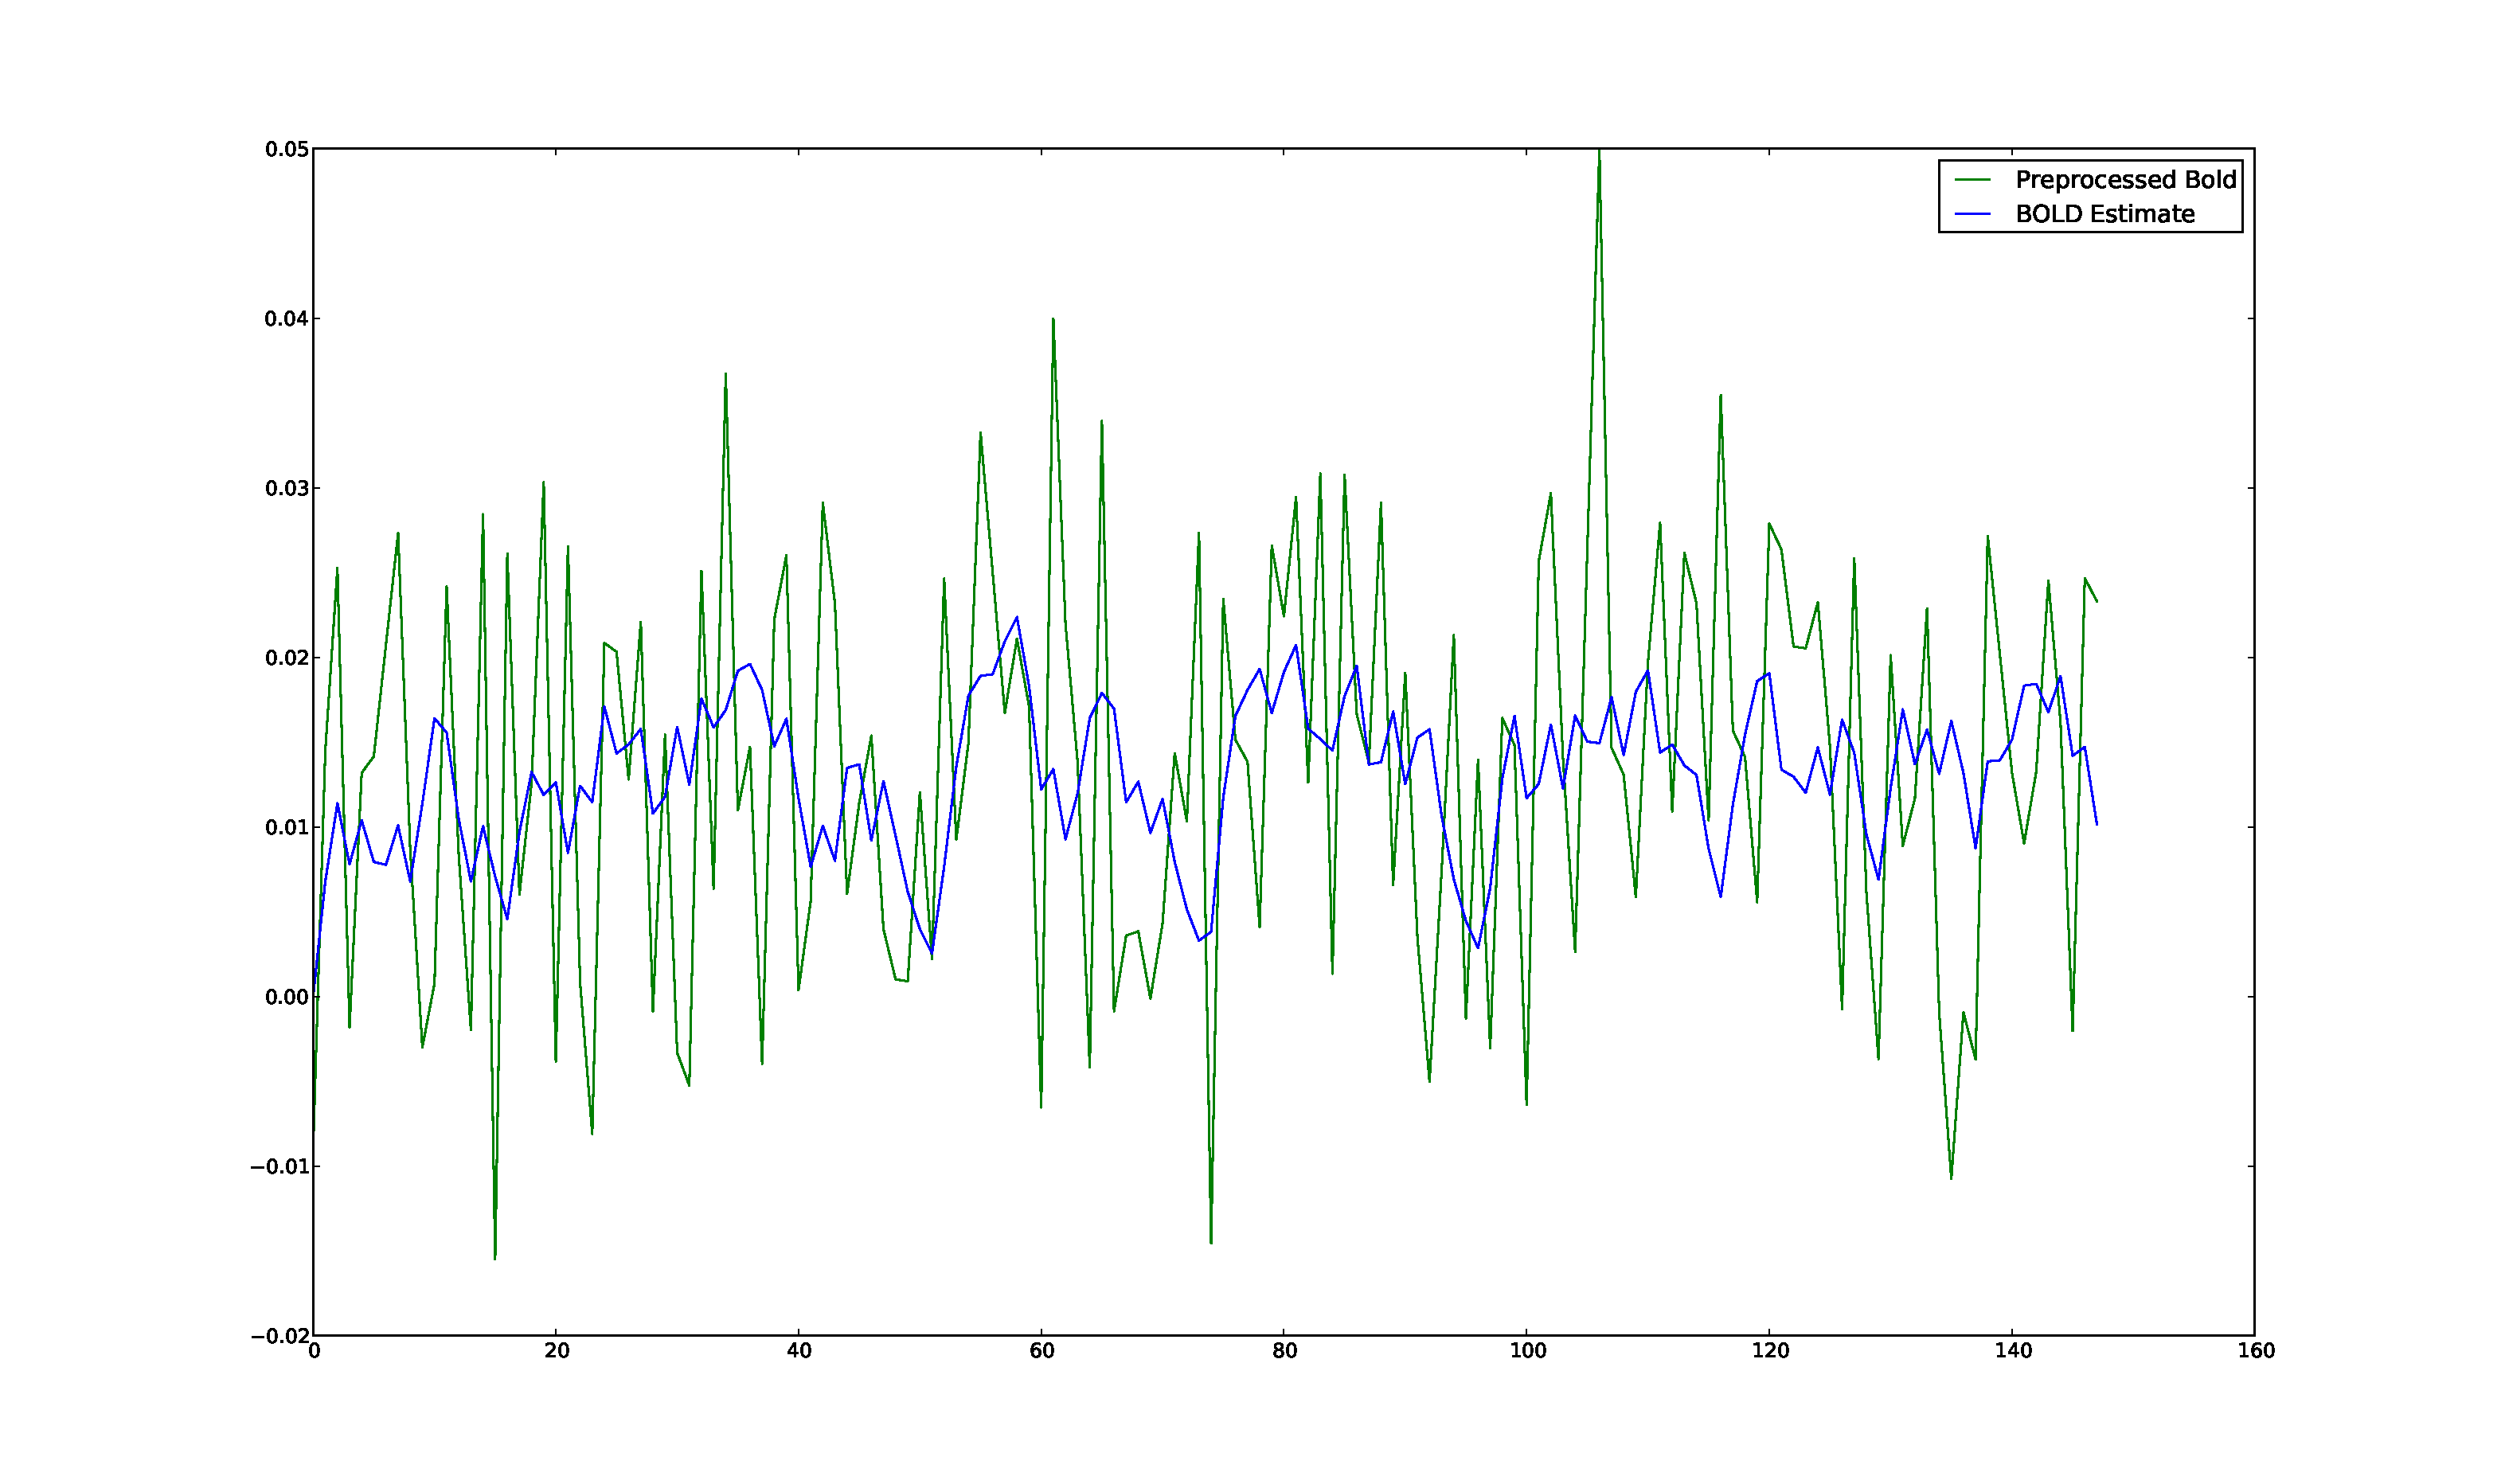
\includegraphics[clip=true,trim=5cm 1cm 4cm 1cm,width=15cm]{images/3_pfilter_23_21_7}}\\
\subfigure[SPM]{\label{fig:comp3spm} 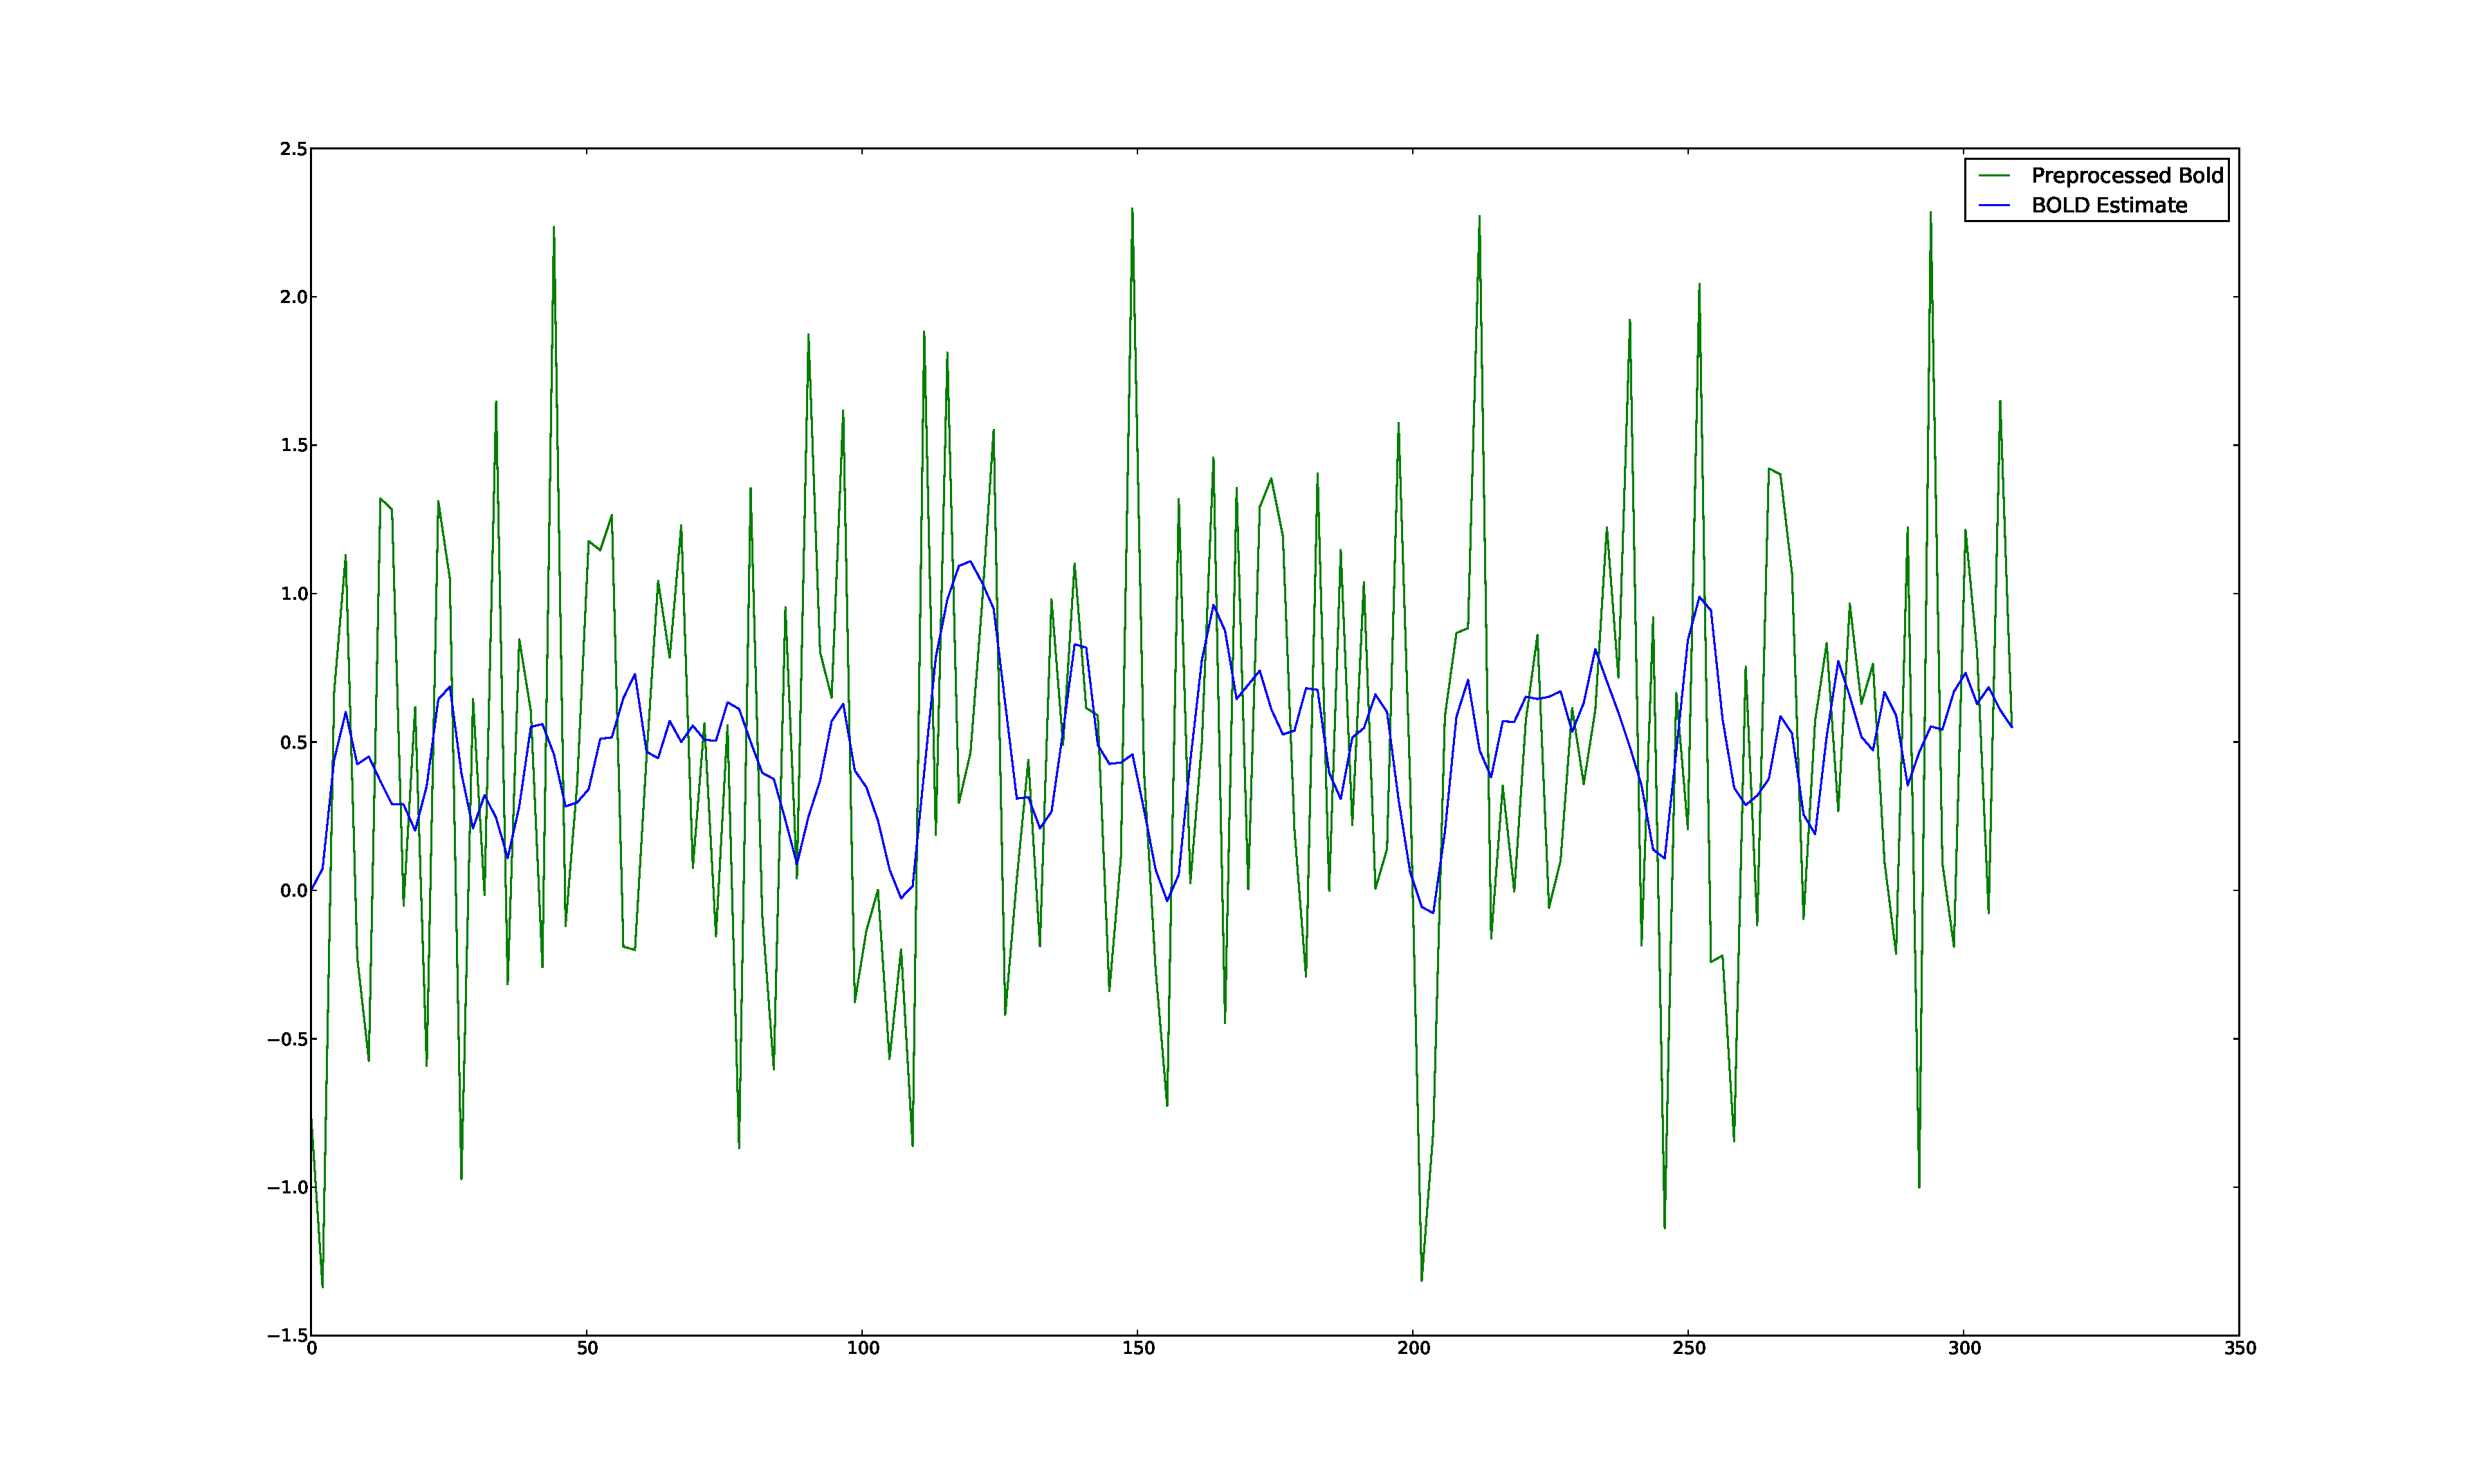
\includegraphics[clip=true,trim=5cm 1cm 4cm 1cm,width=15cm]{images/3_spm_23_21_7}}
\caption{Section 3, Estimated vs. Actual BOLD response}
\label{fig:comp3}
\end{figure}

\begin{figure}[H]
\subfigure[Particle Filter]{\label{fig:comp4pfilter} 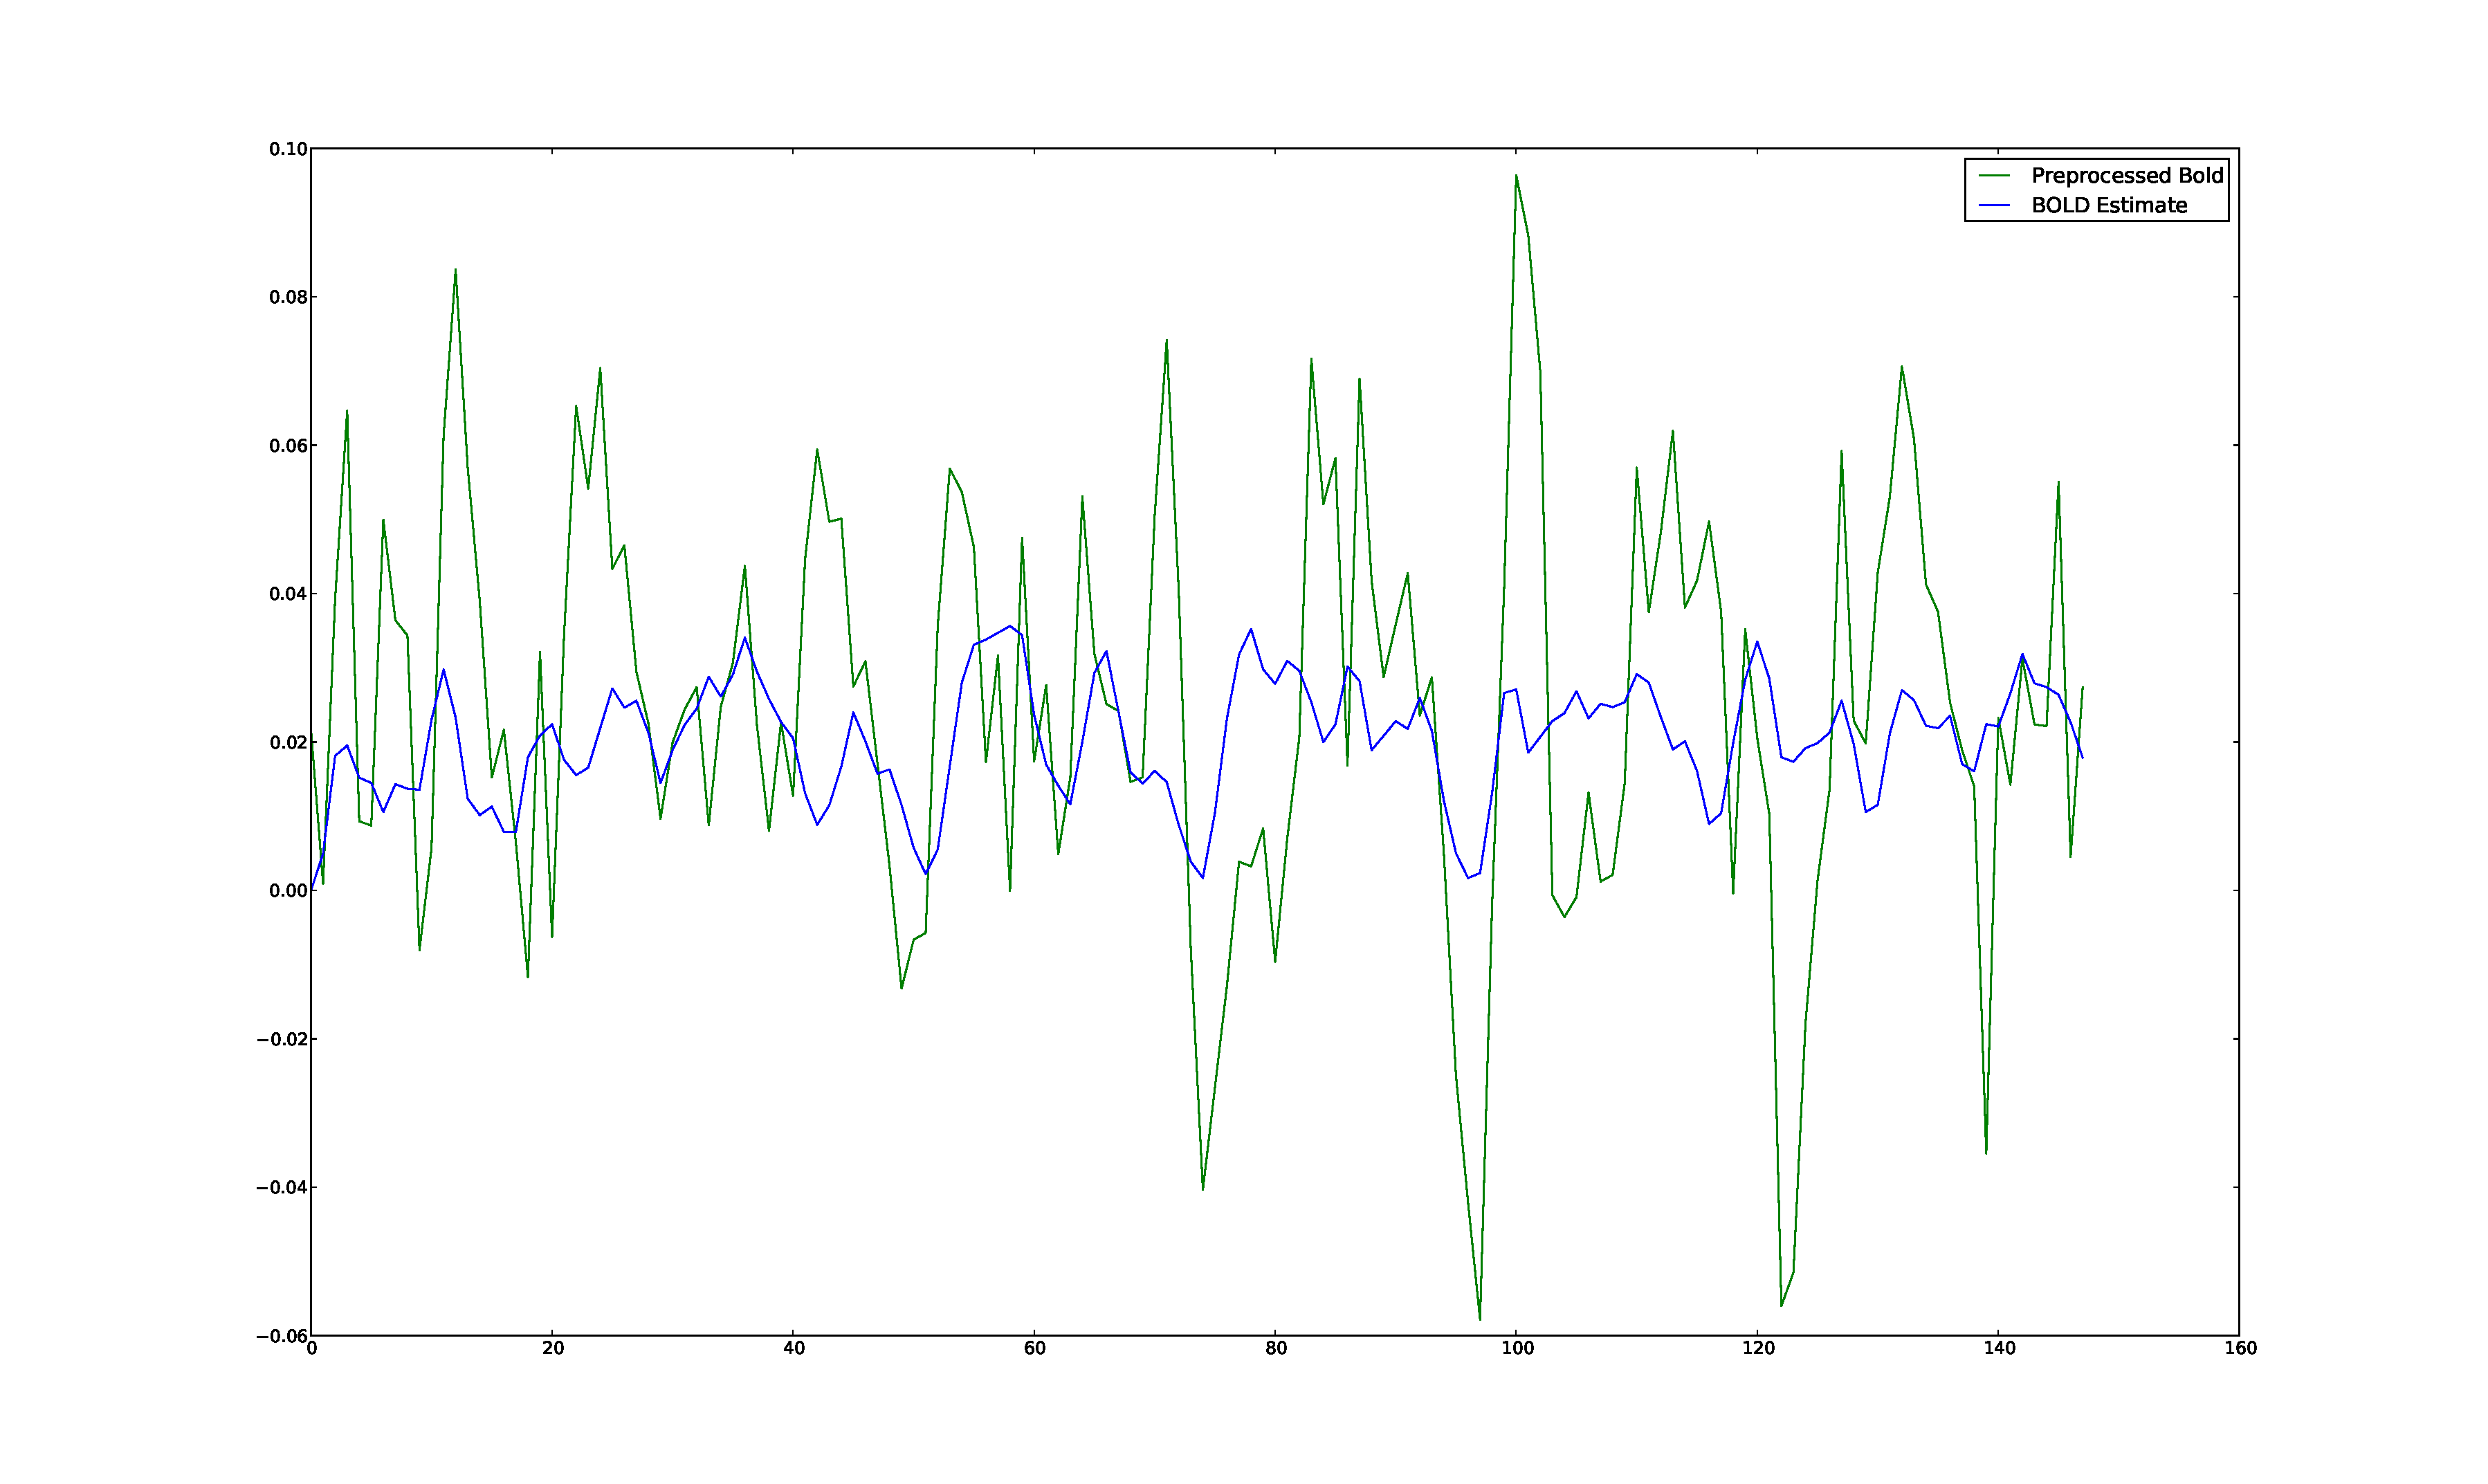
\includegraphics[clip=true,trim=5cm 1cm 4cm 1cm,width=15cm]{images/4_pfilter_26_15_7}}\\
\subfigure[SPM]{\label{fig:comp4spm} 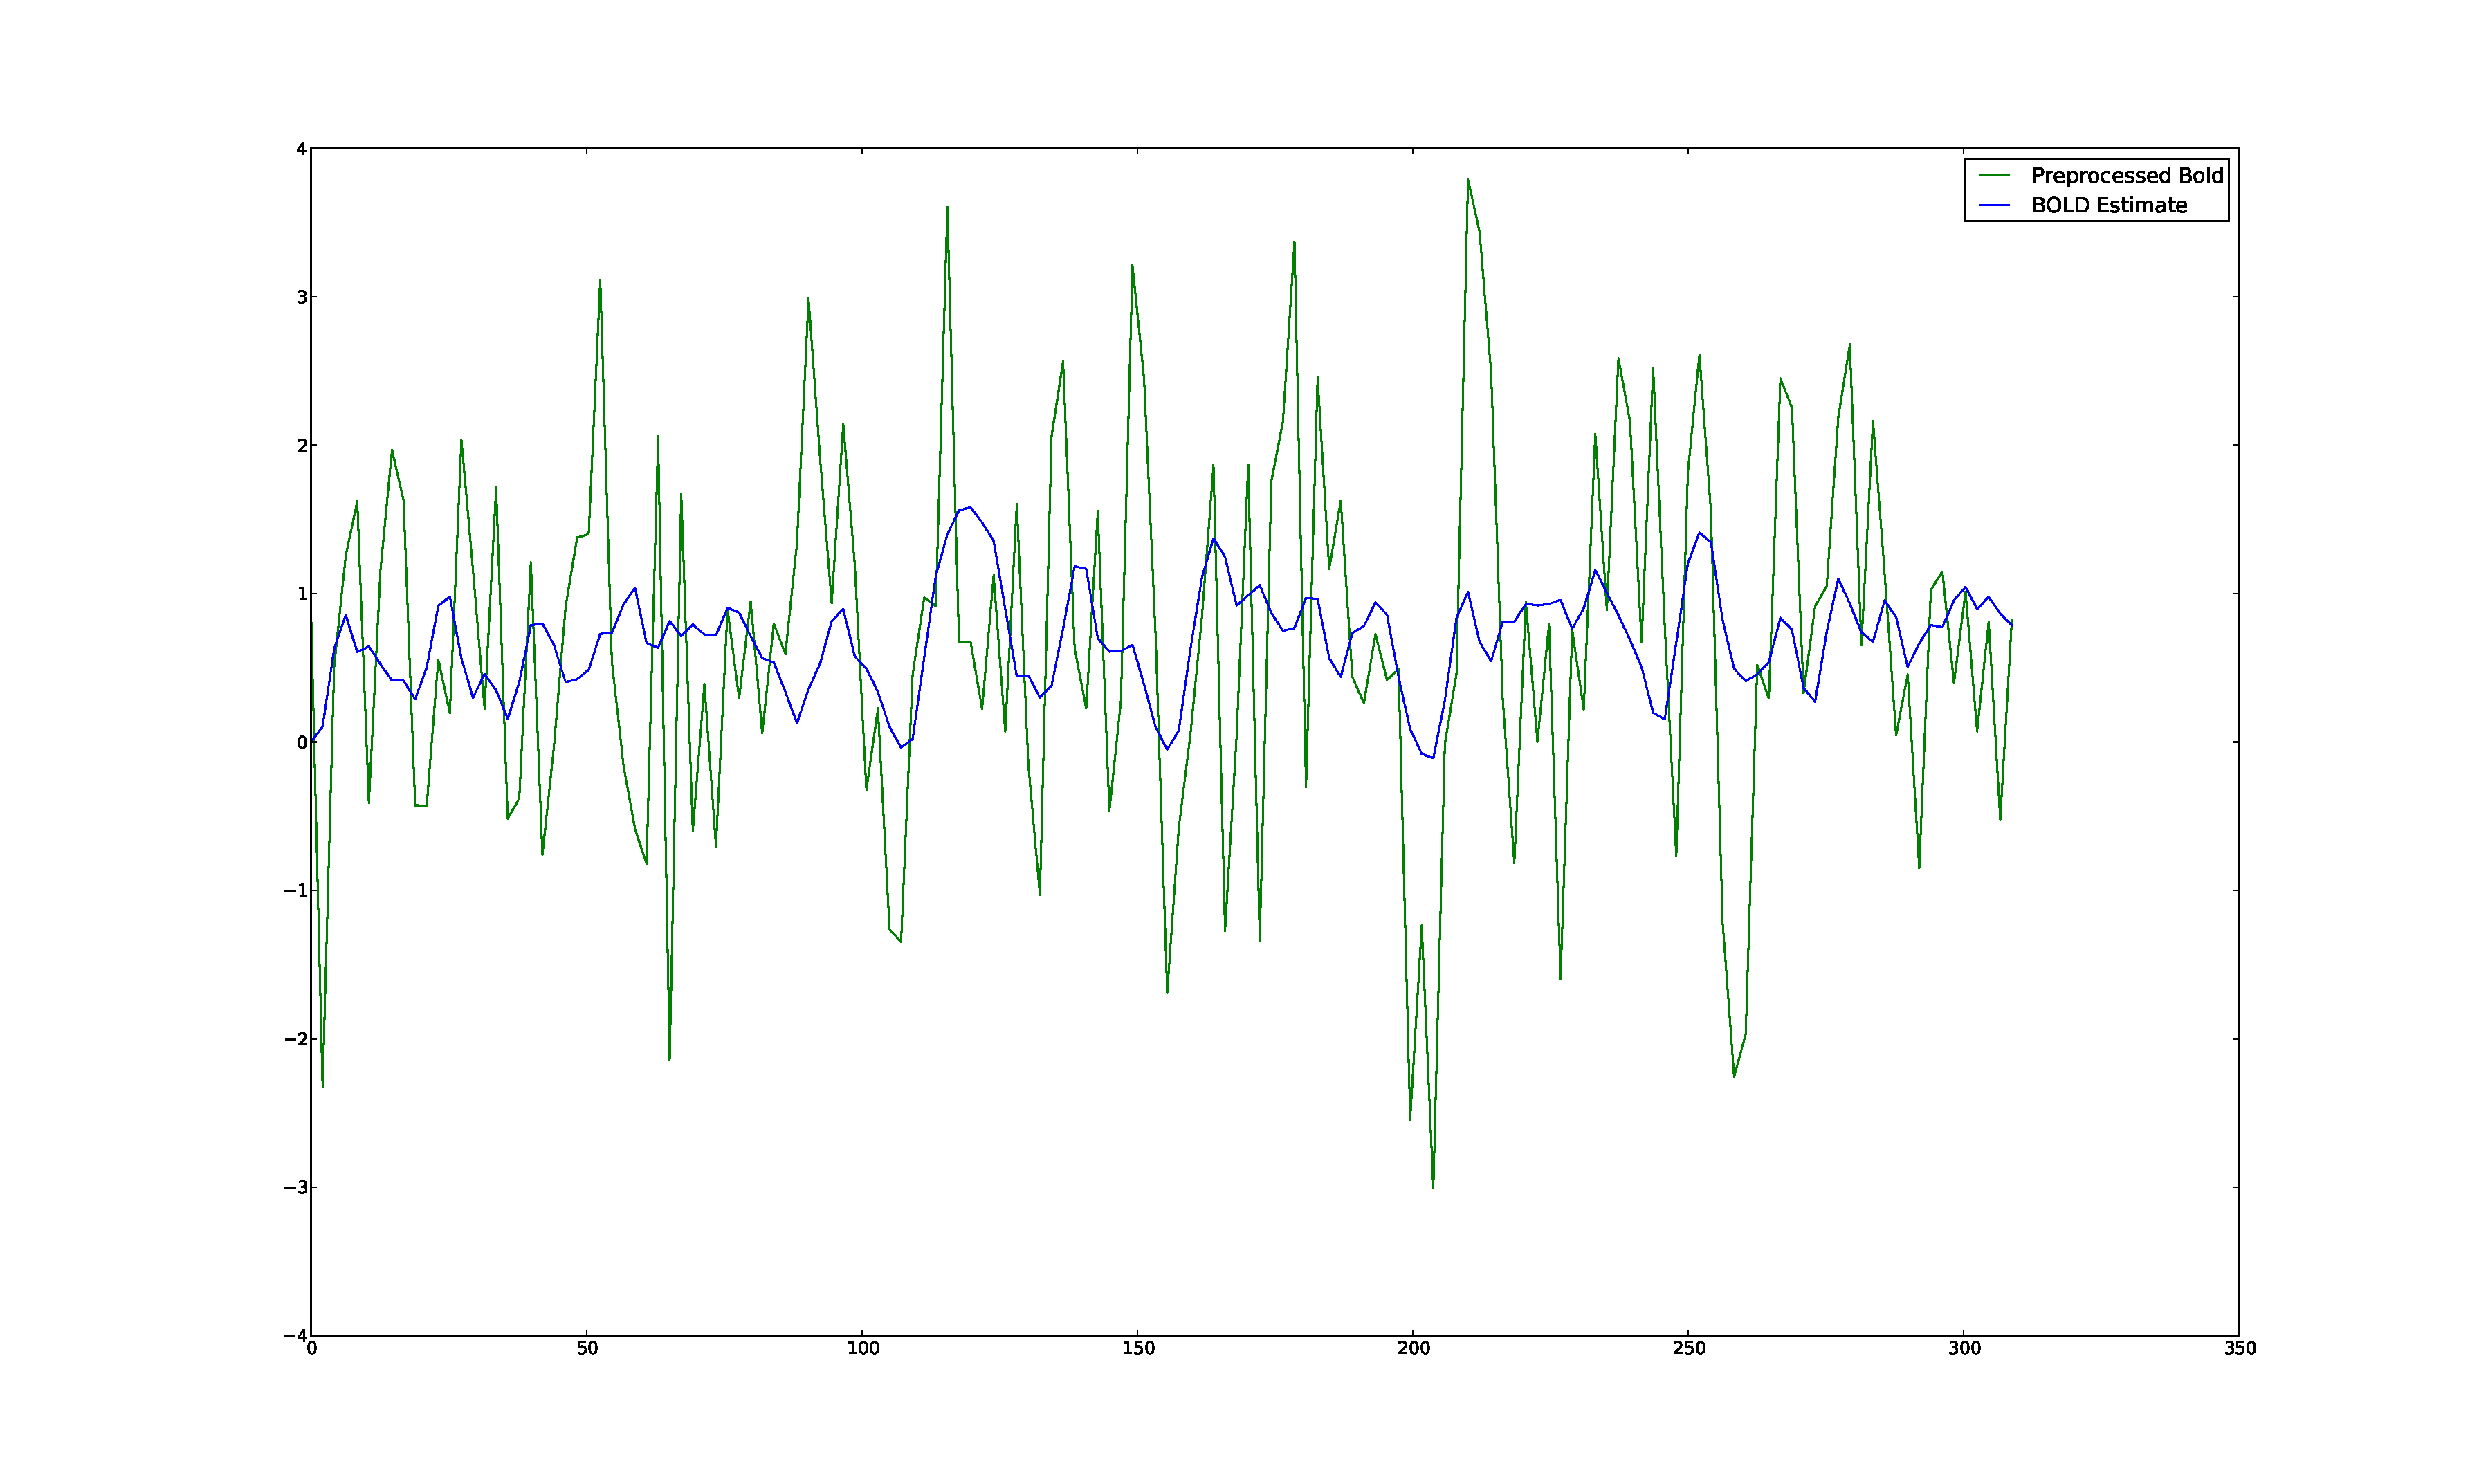
\includegraphics[clip=true,trim=5cm 1cm 4cm 1cm,width=15cm]{images/4_spm_26_15_7}}
\caption{Section 4, Estimated vs. Actual BOLD response}
\label{fig:comp4}
\end{figure}

% or in original coordinates 29-9-13
\begin{figure}
\subfigure[Particle Filter]{\label{fig:comp5pfilter} 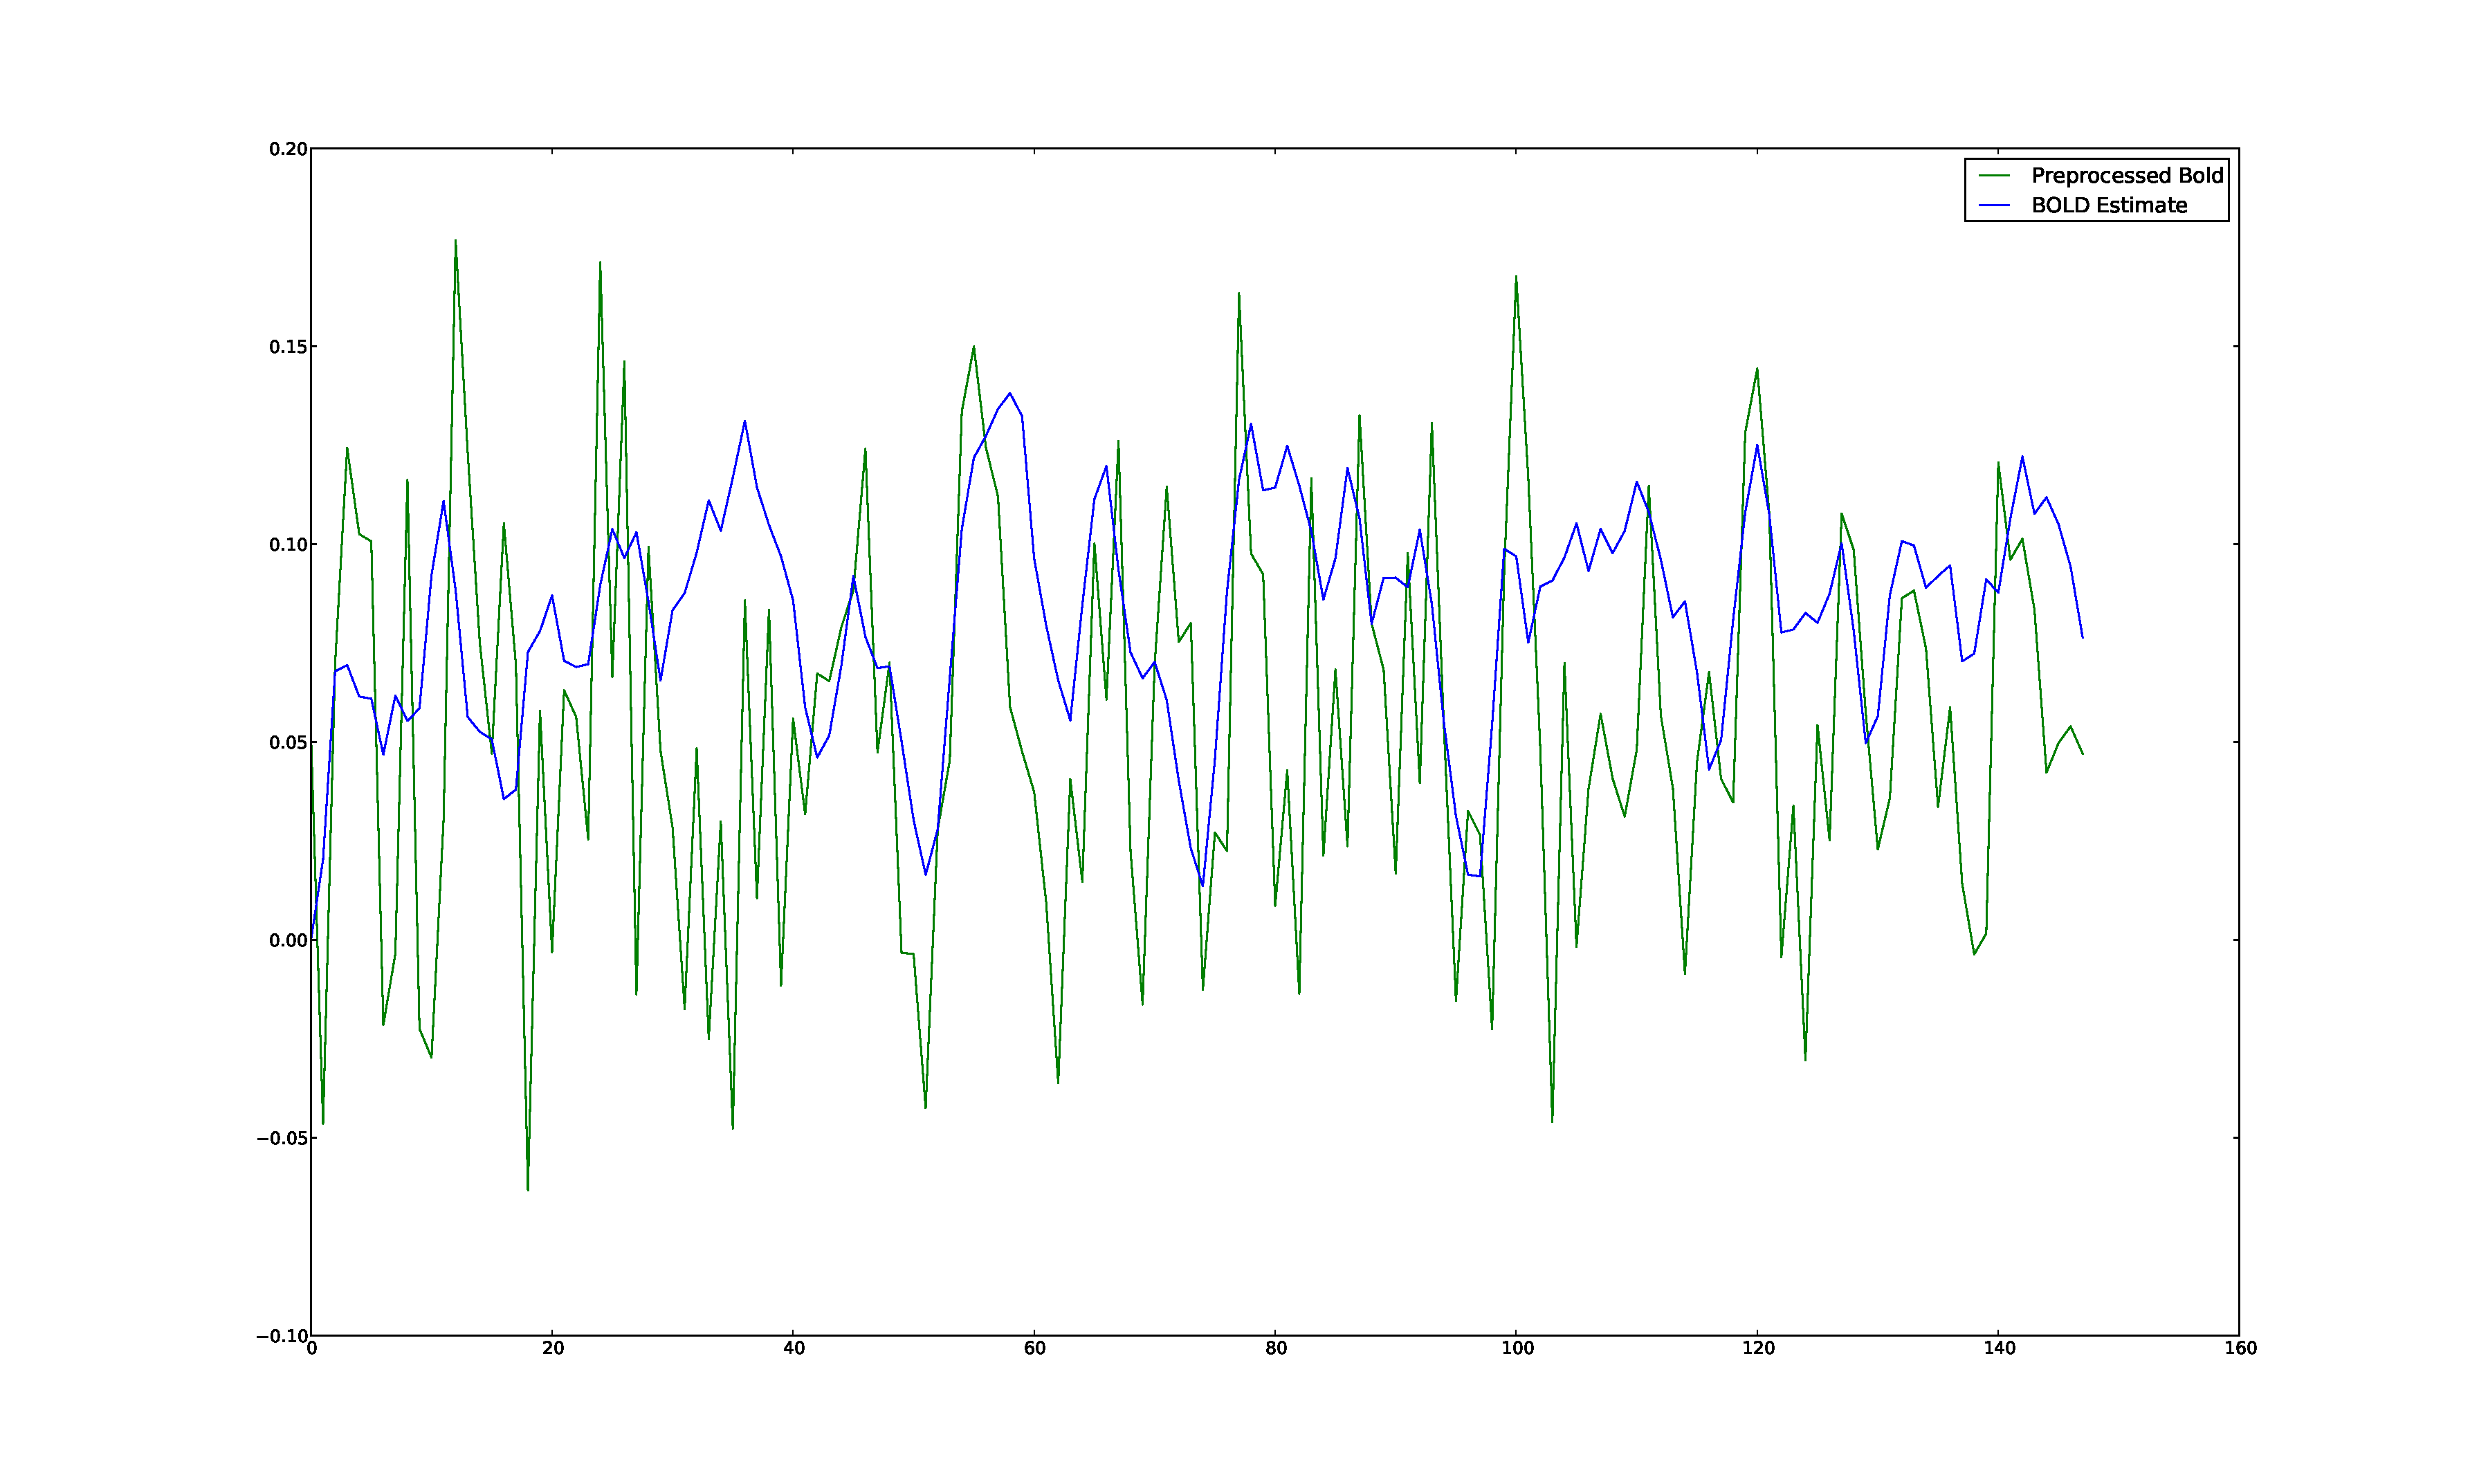
\includegraphics[clip=true,trim=5cm 1cm 4cm 1cm,width=15cm]{images/5_pfilter_29_9_13}}\\
\subfigure[SPM]{\label{fig:comp5spm} 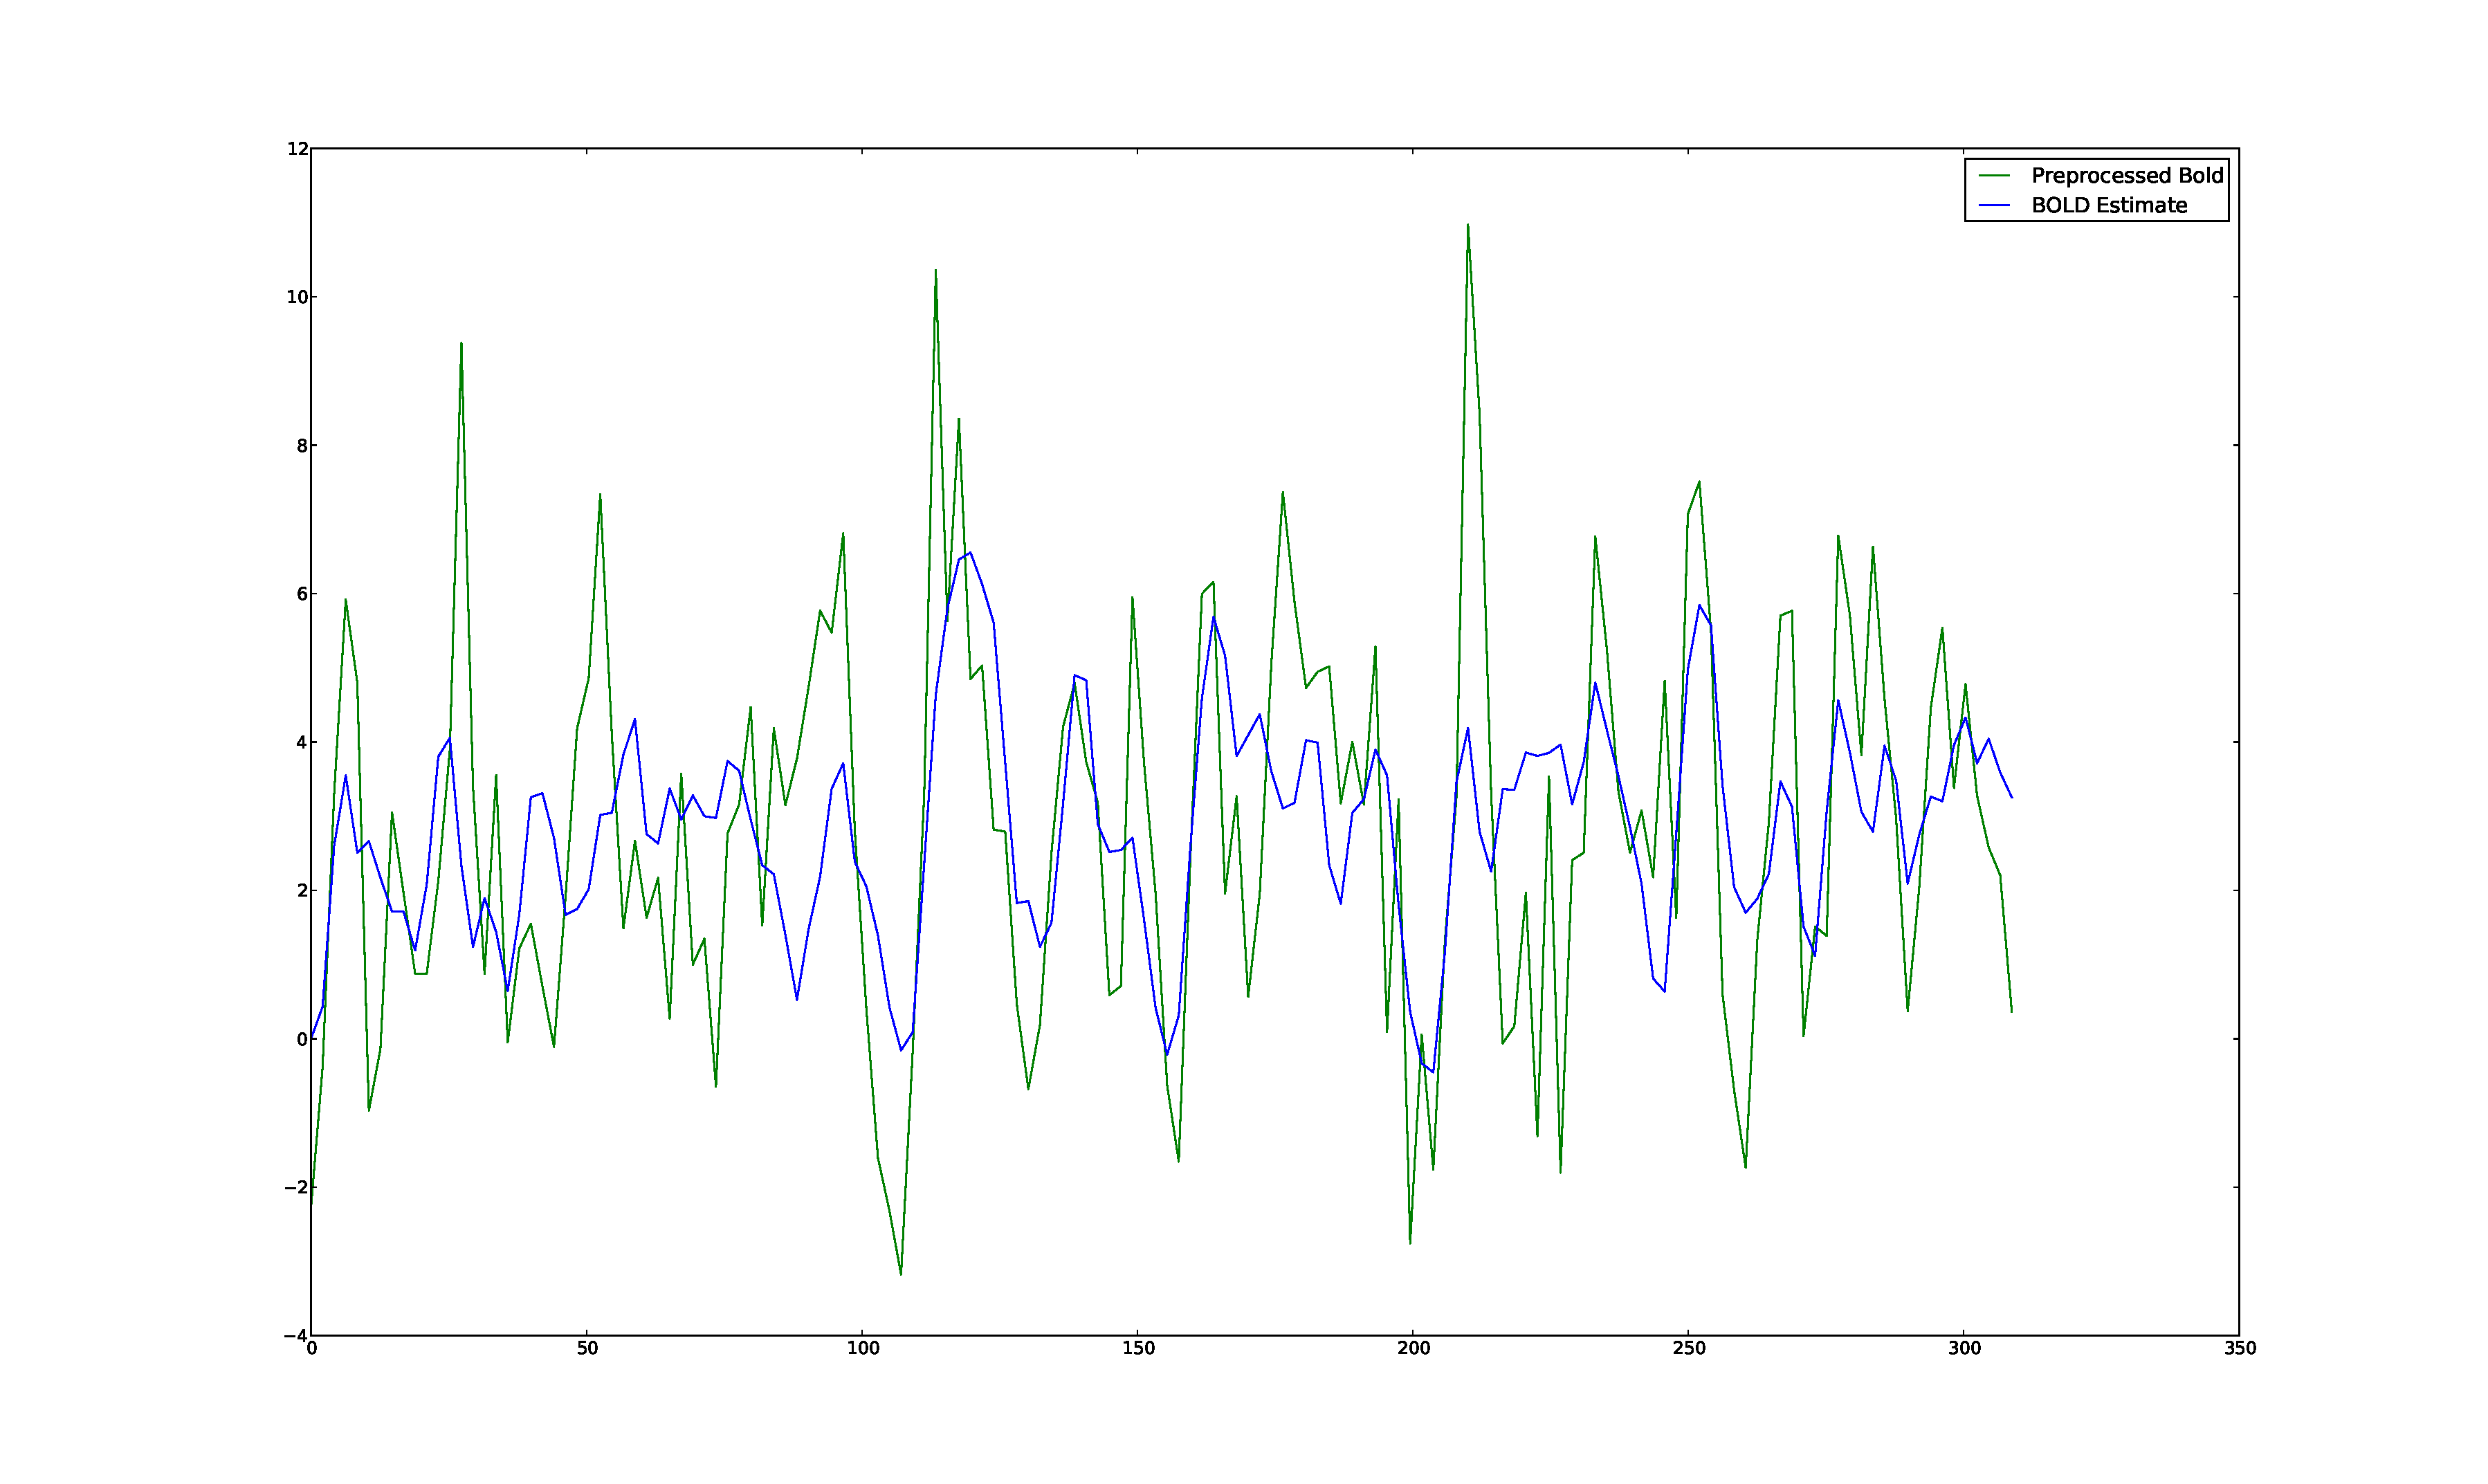
\includegraphics[clip=true,trim=5cm 1cm 4cm 1cm,width=15cm]{images/5_spm_29_9_13}}
\caption{Section 5, Below threshold in both particle filter checks, but above threshold in SPM. Mutual Information of $0.0212822$, T-Value
of $4.17399$ and $MSE$ of $1.14171$.}
\label{fig:comp5}
\end{figure}

%23-10-18 or in original coordinates 36-17-19
\begin{figure}
\subfigure[Particle Filter]{\label{fig:comp5pfilter} 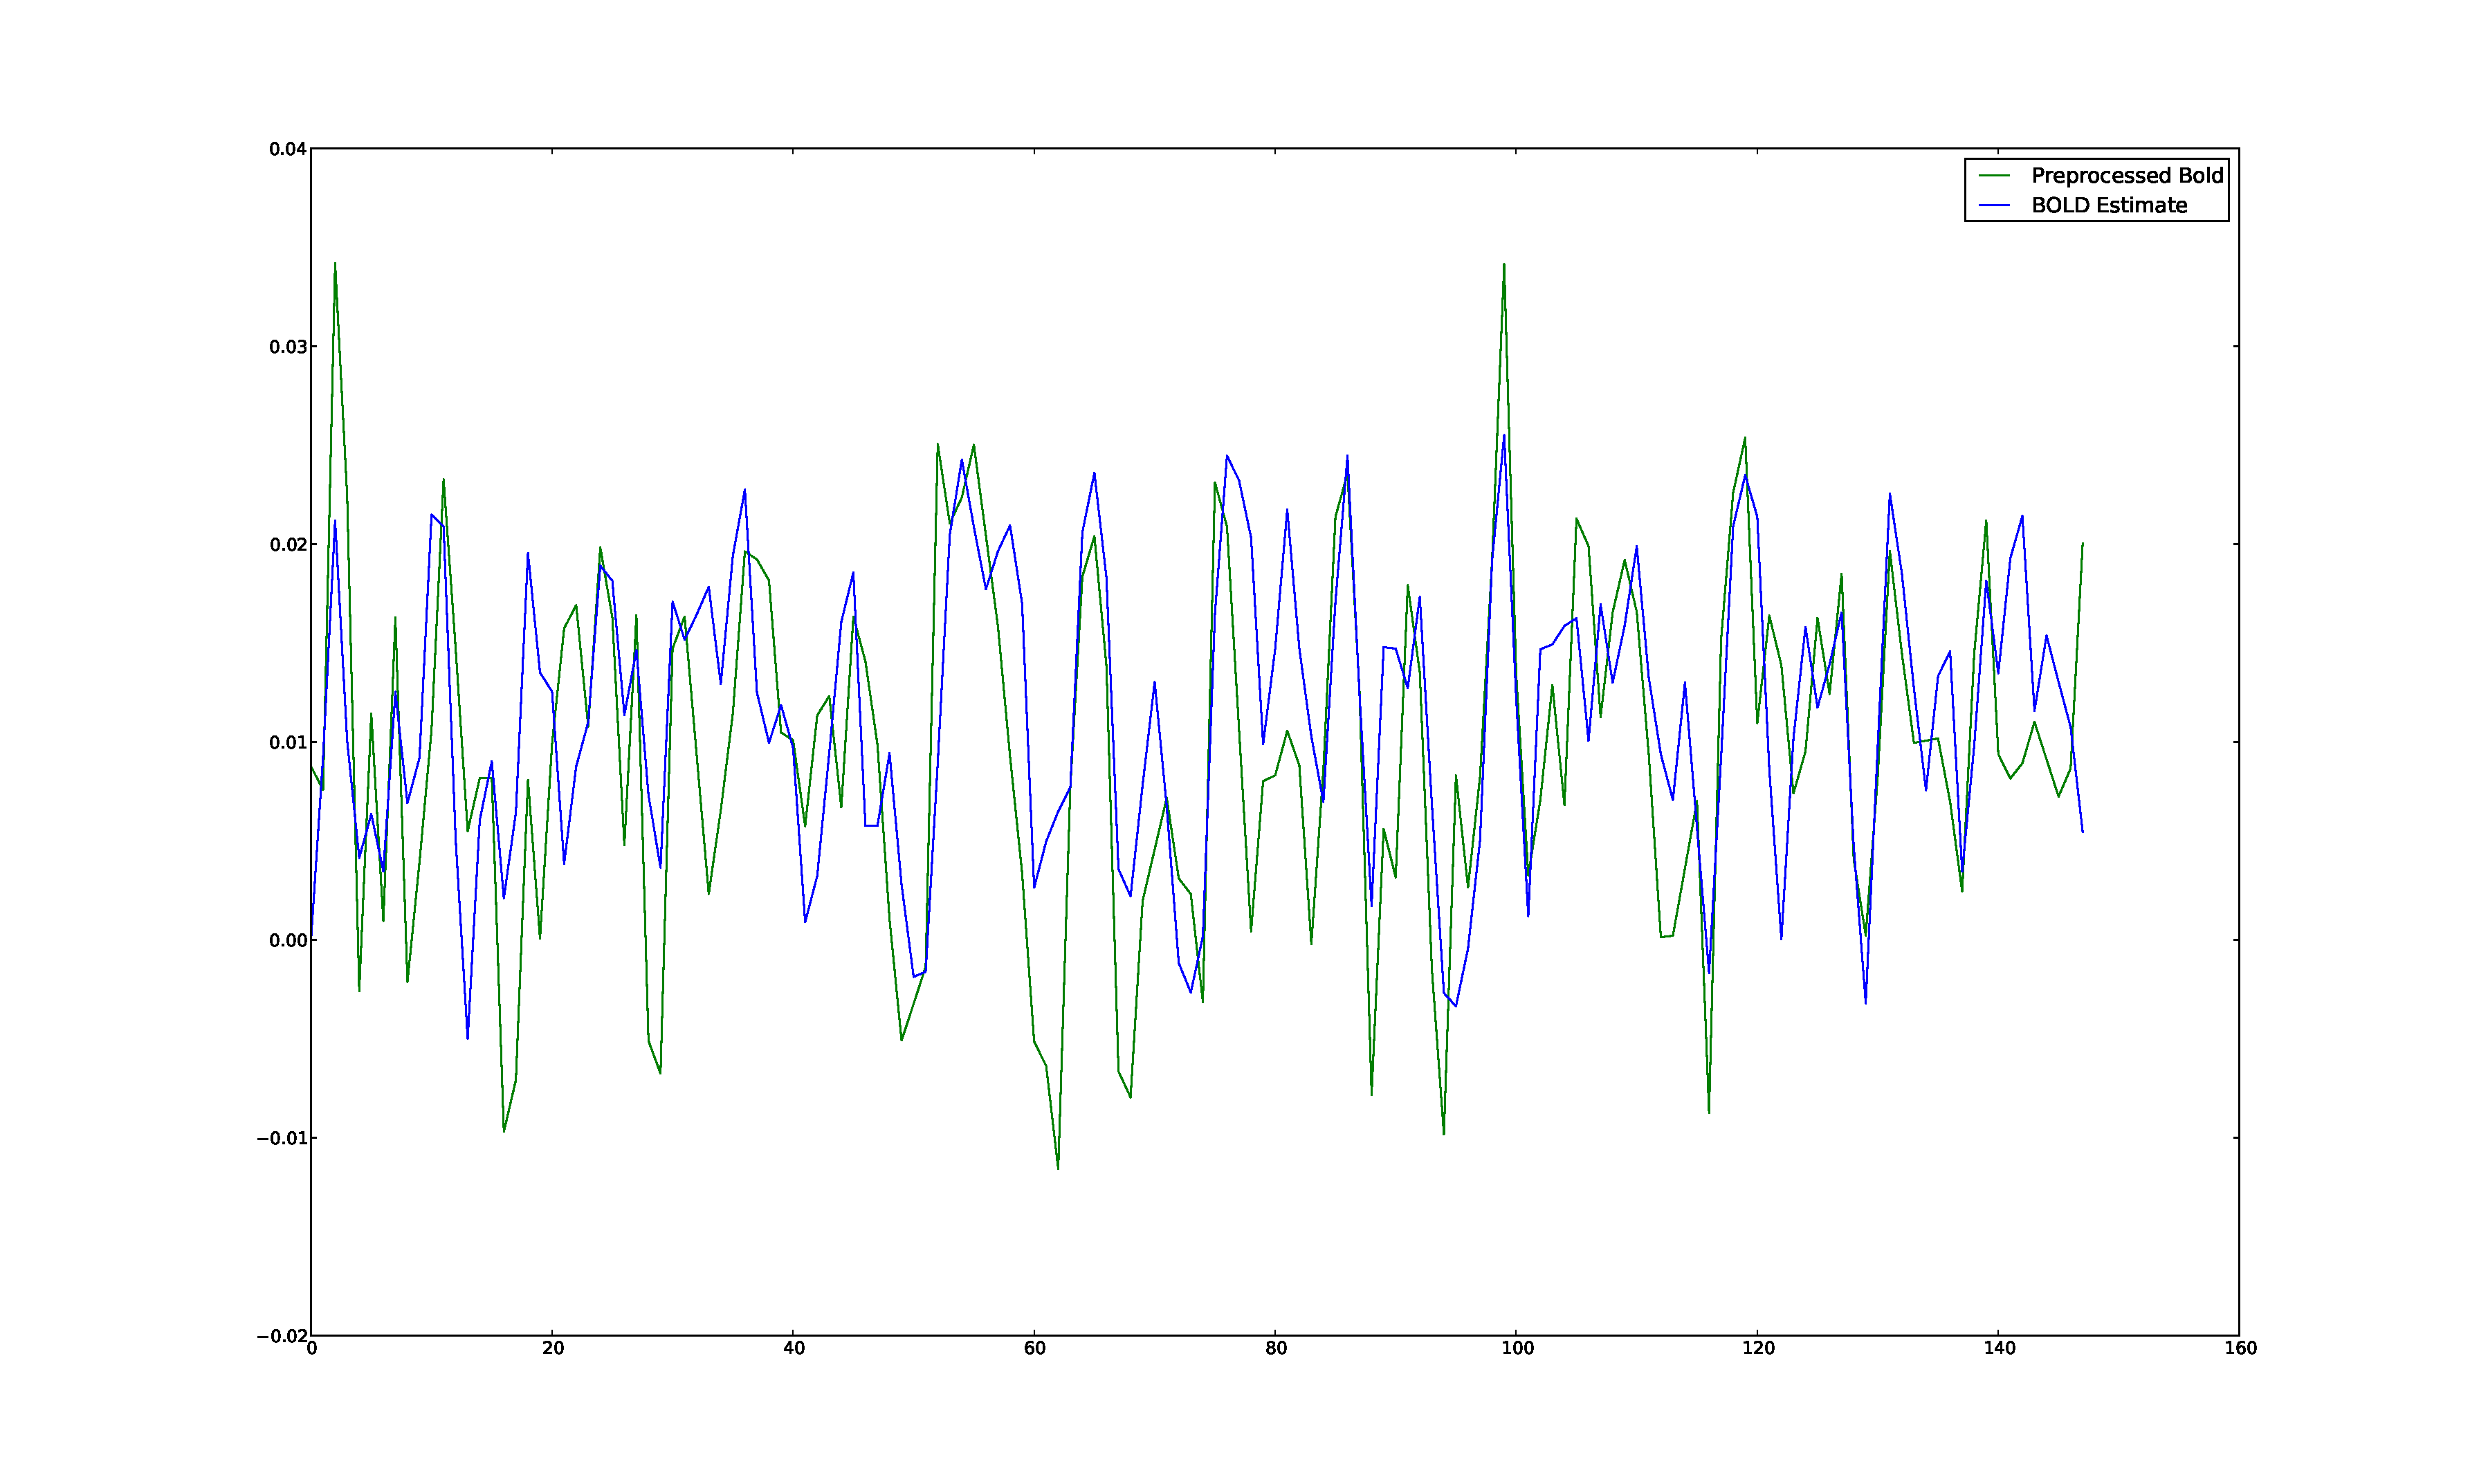
\includegraphics[clip=true,trim=5cm 1cm 4cm 1cm,width=15cm]{images/6_pfilter_36_17_19}}\\
\subfigure[SPM]{\label{fig:comp5spm} 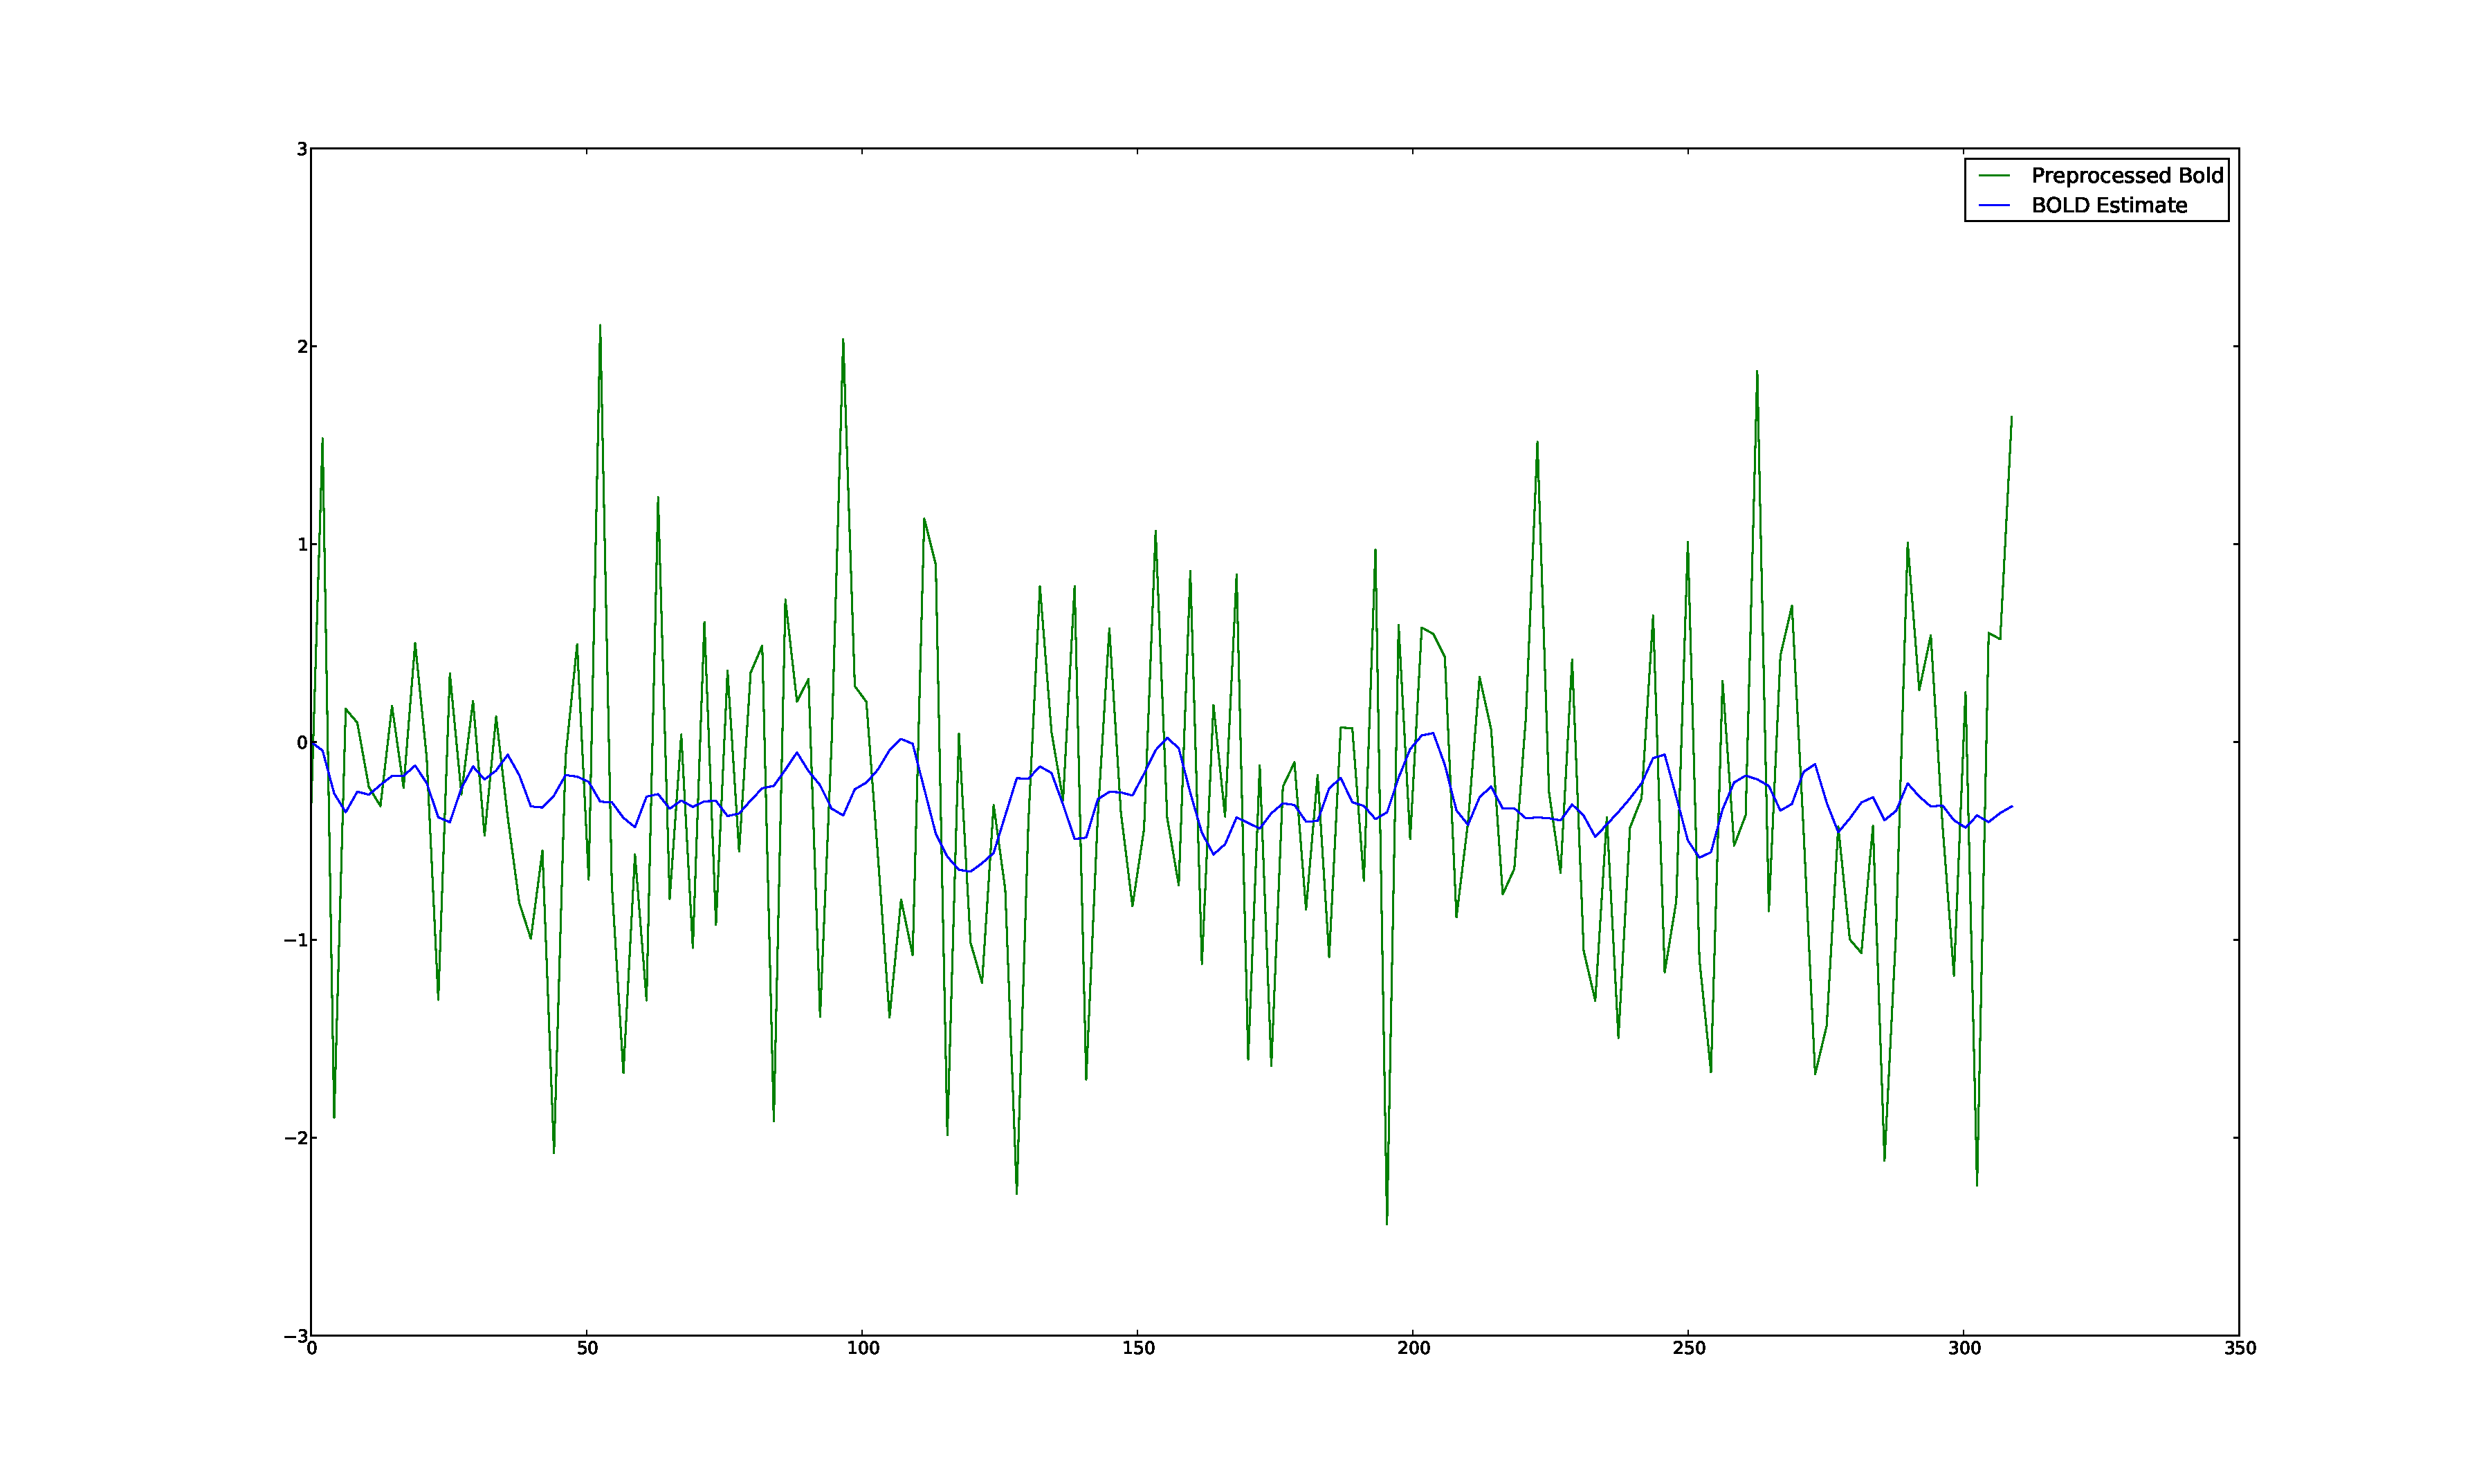
\includegraphics[clip=true,trim=5cm 1cm 4cm 1cm,width=15cm]{images/6_spm_36_17_19}}
\caption{Section 6, MI of $0.335504$, T Value: $2.49154$, normalized error: $0.783348$ Not visible in SPM}
\label{fig:comp6}
\end{figure}

%16-19-0 or in original coordinates 29-26-1
\begin{figure}
\subfigure[Particle Filter]{\label{fig:comp5pfilter} 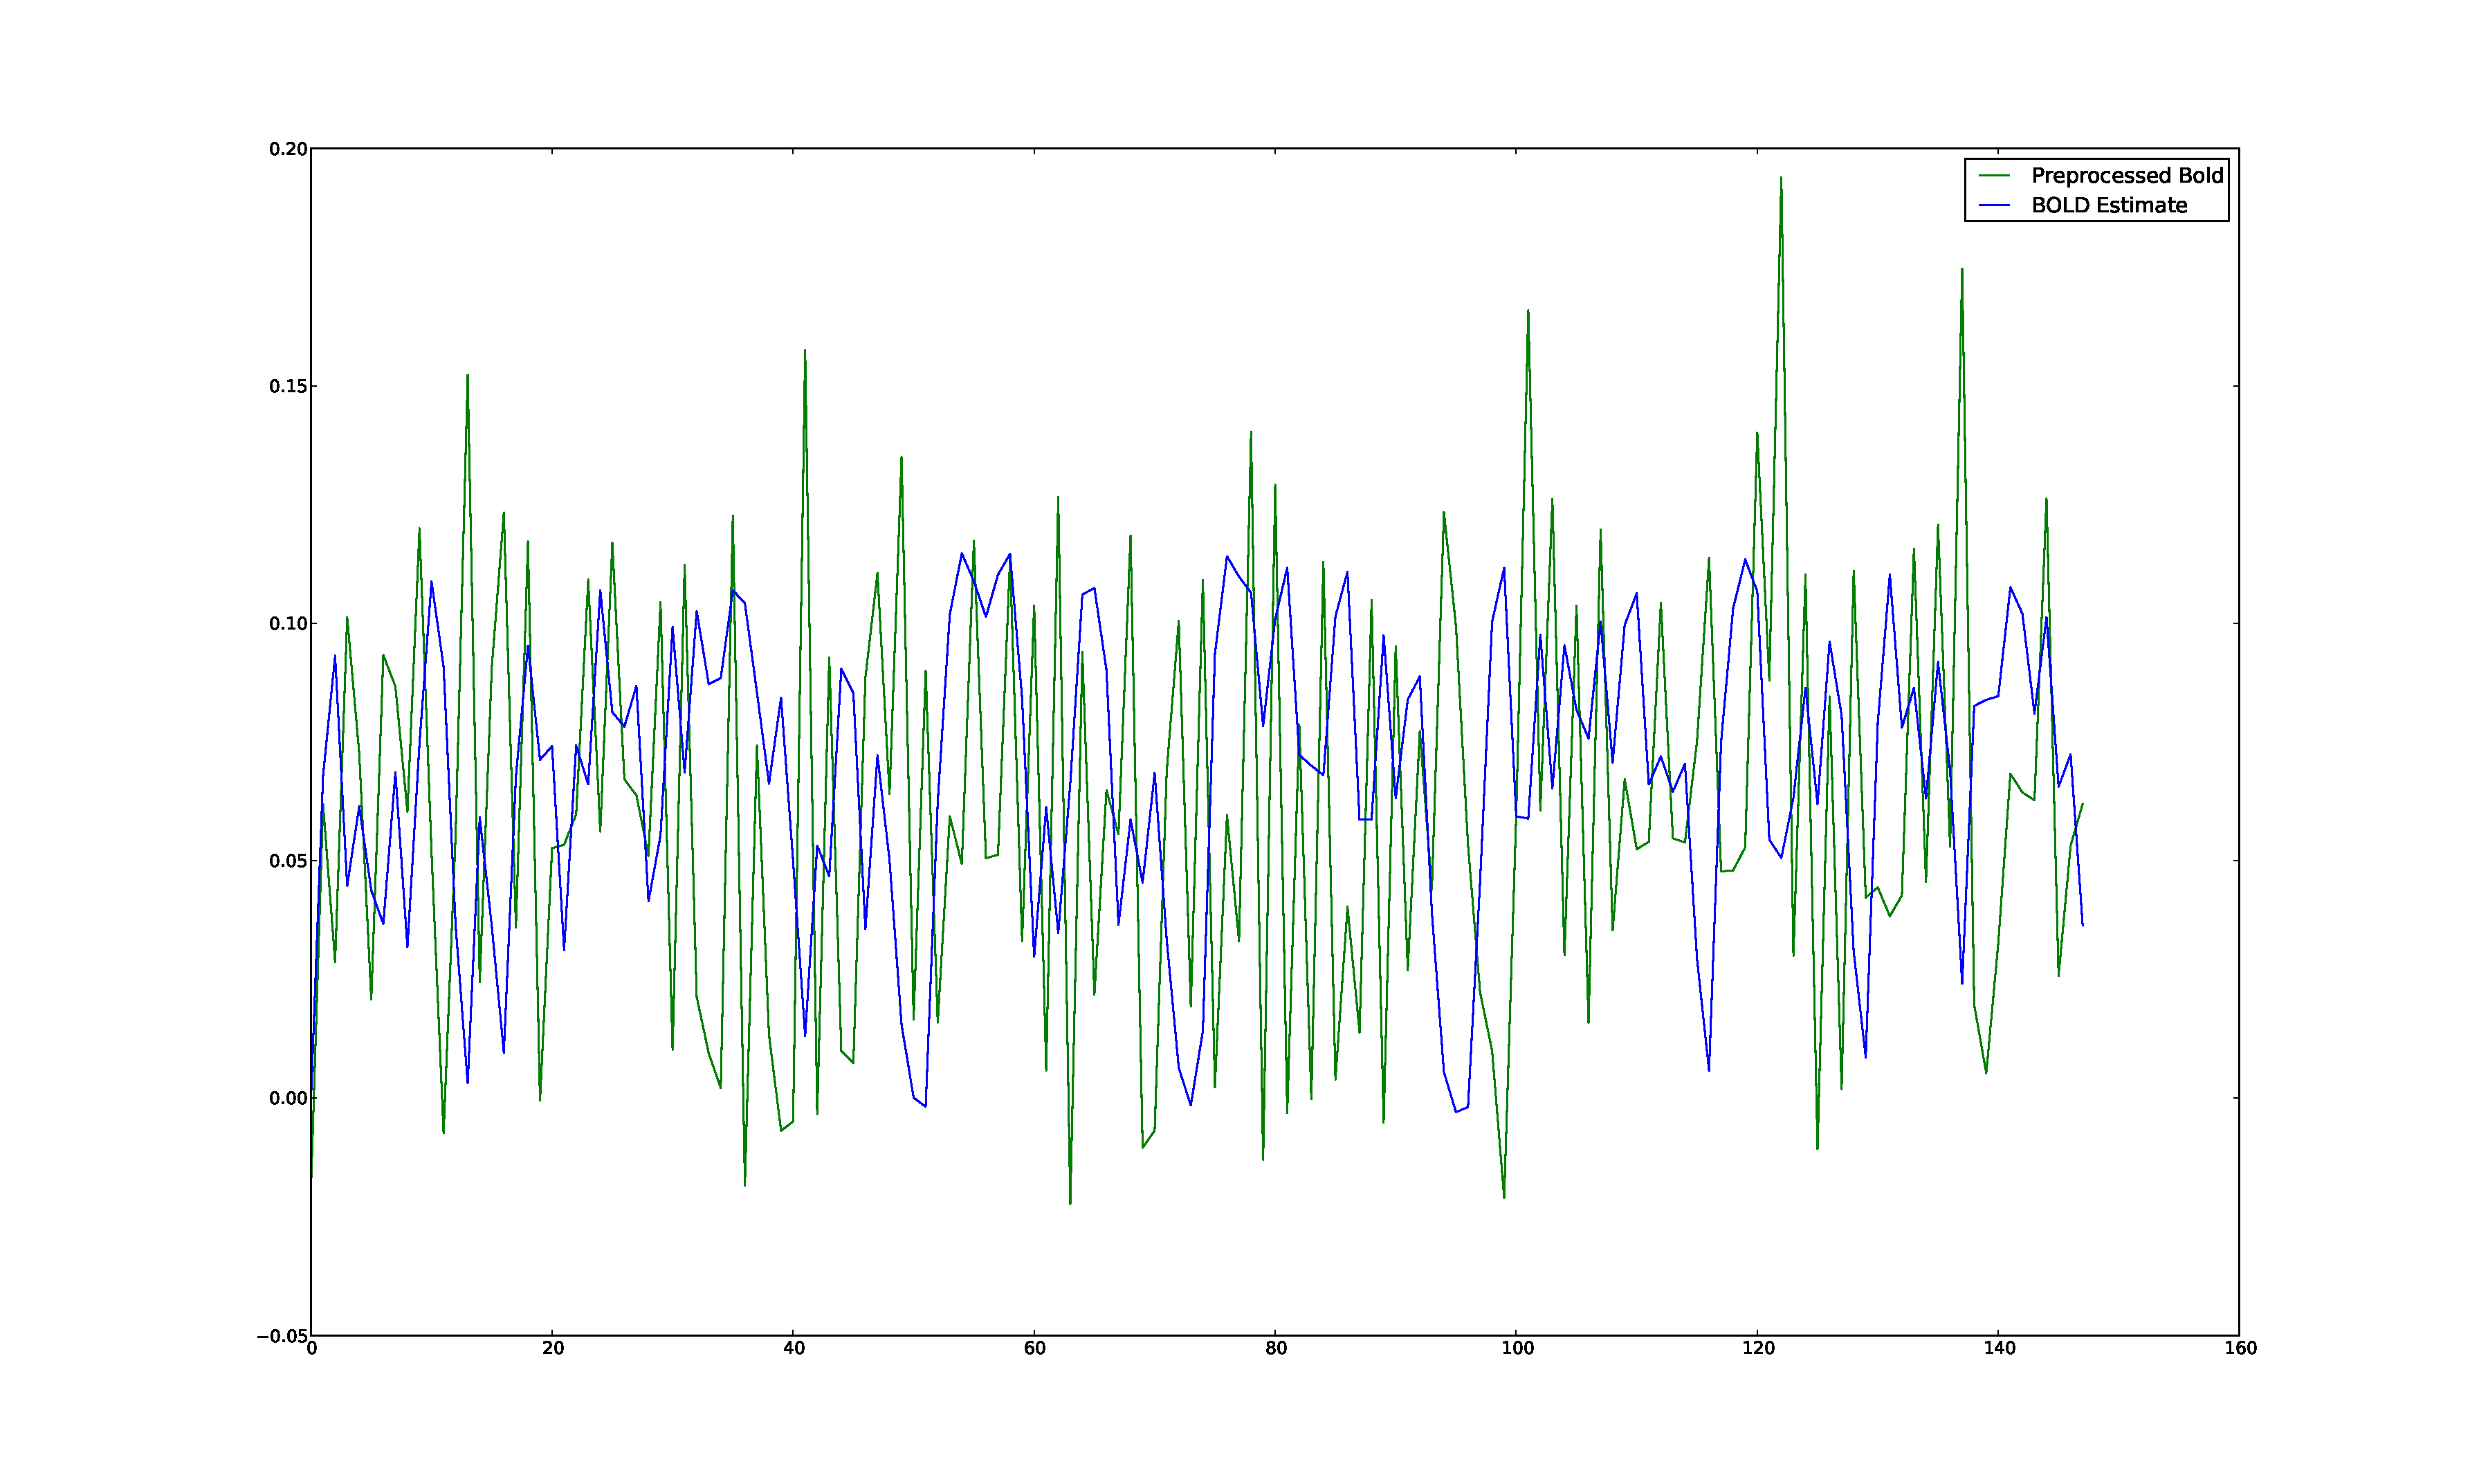
\includegraphics[clip=true,trim=5cm 1cm 4cm 1cm,width=15cm]{images/7_pfilter_29_26_1}}\\
%\subfigure[SPM]{\label{fig:comp5spm} 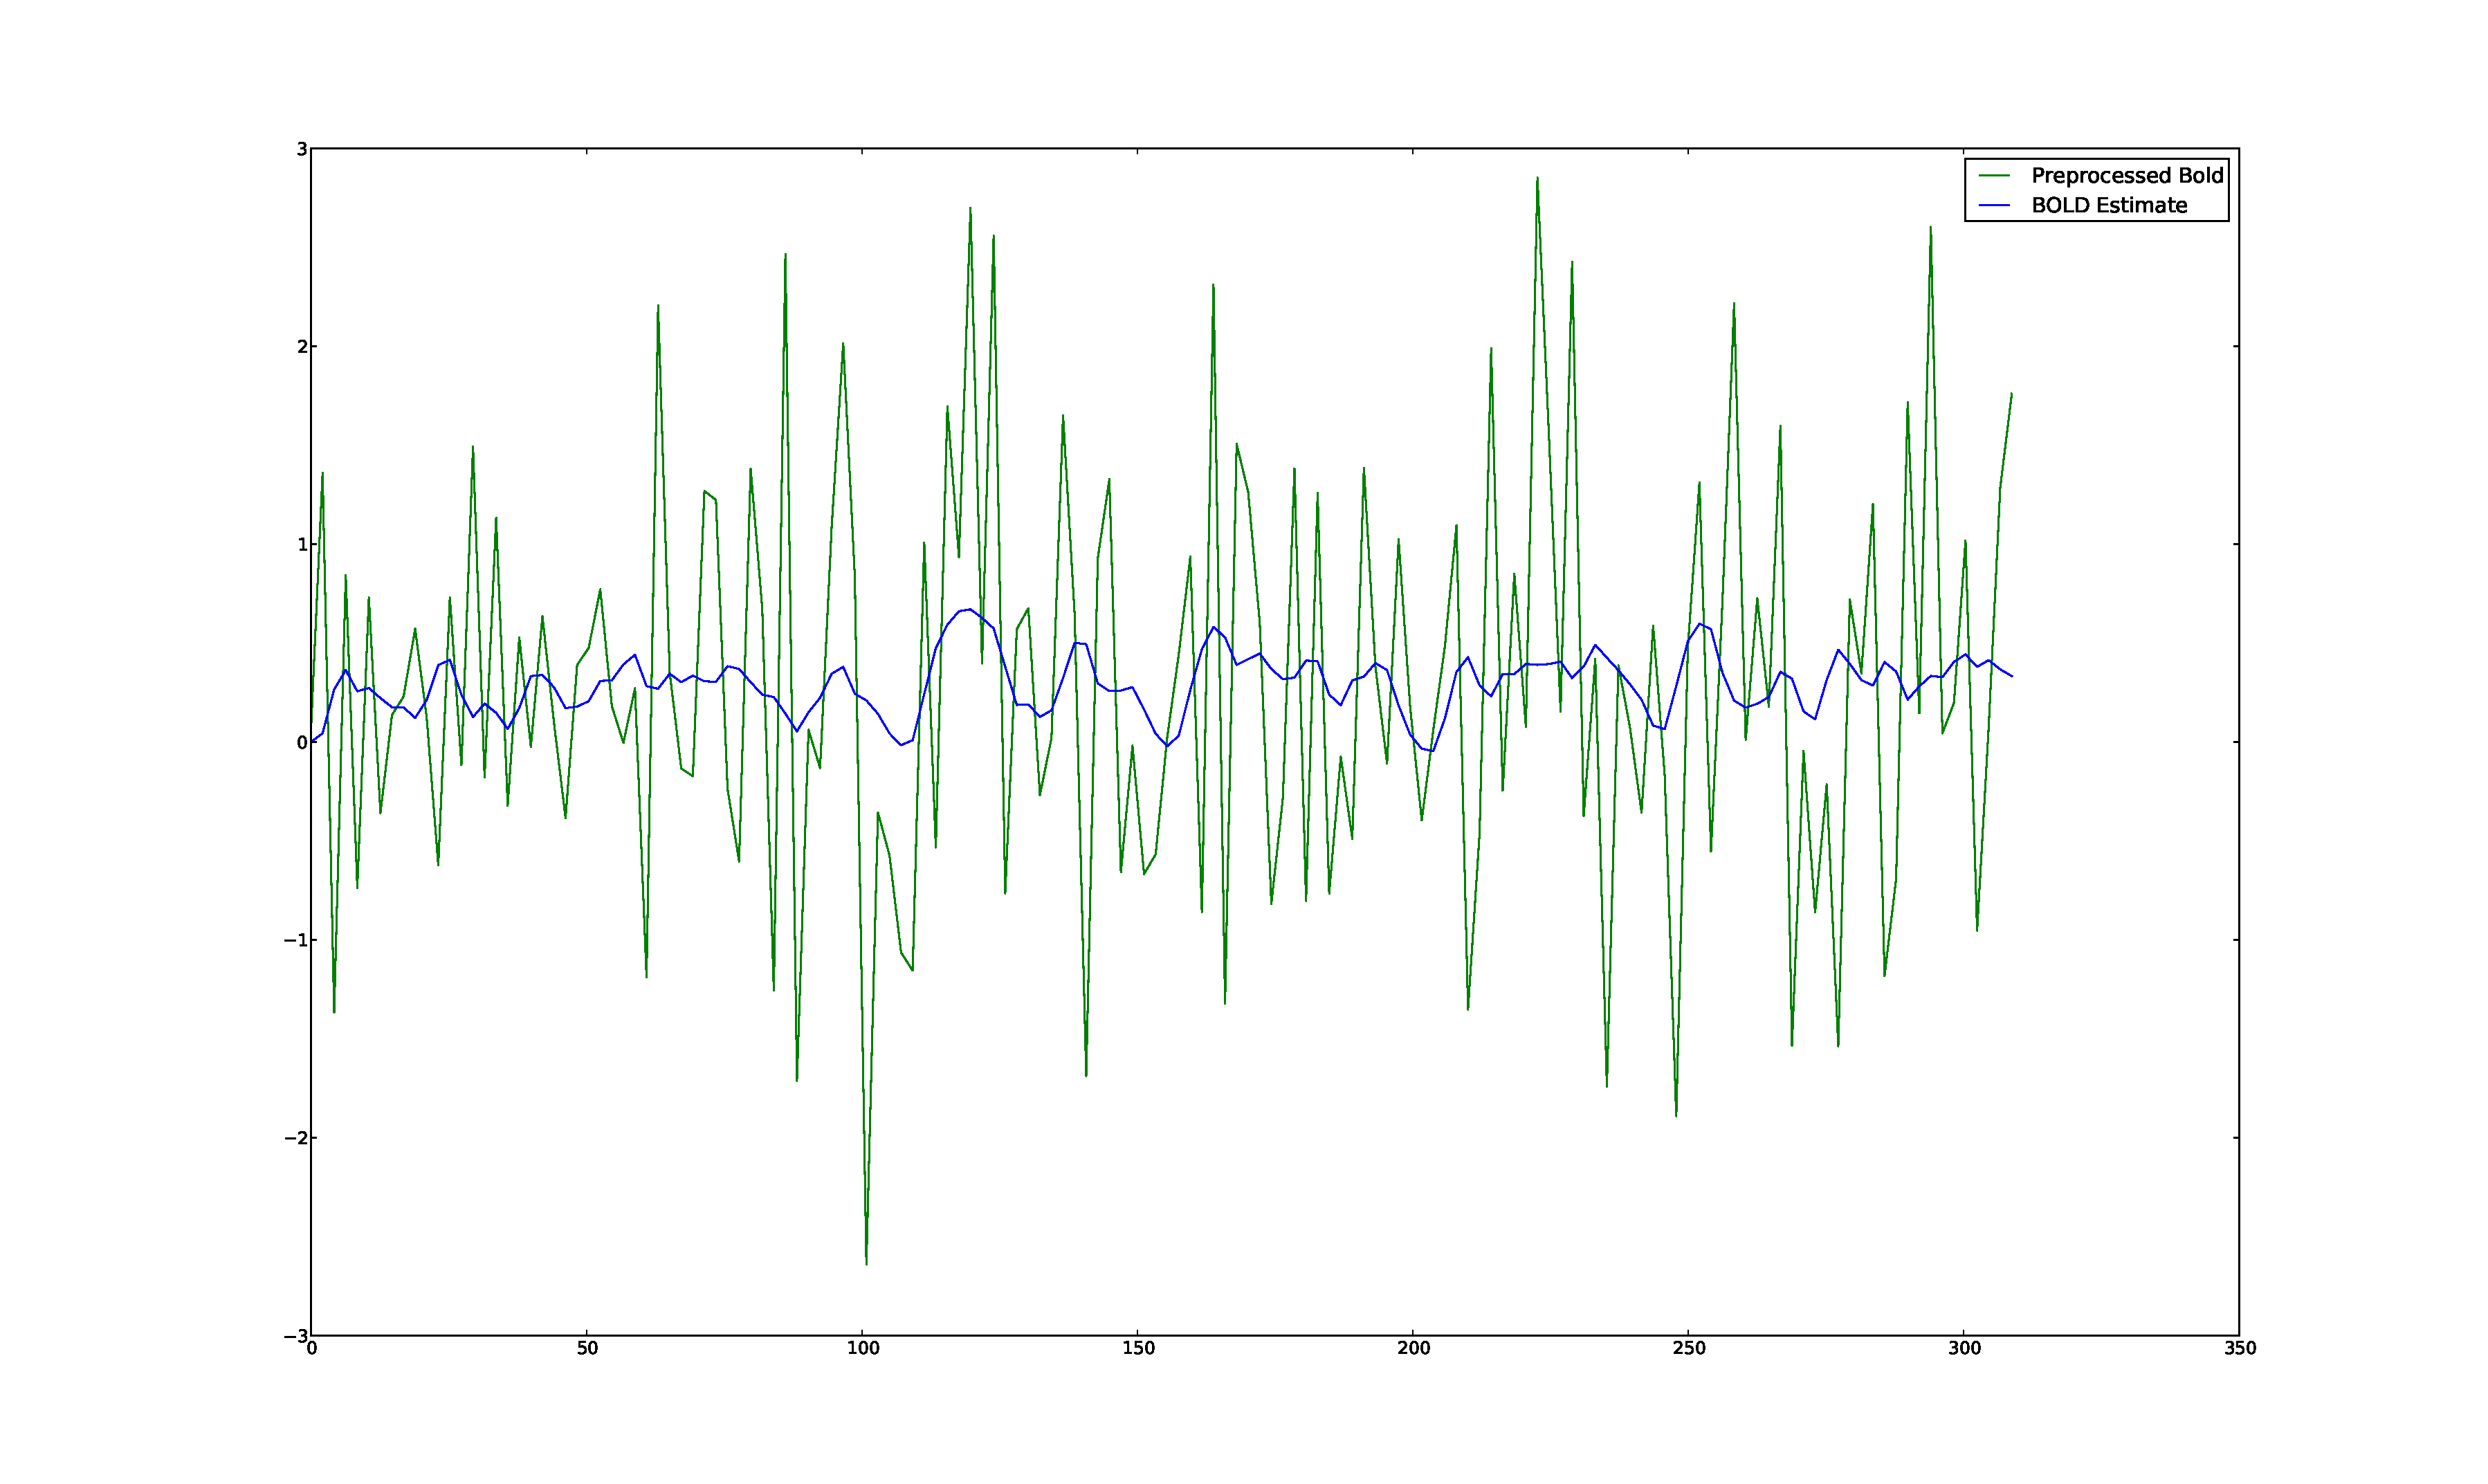
\includegraphics[clip=true,trim=5cm 1cm 4cm 1cm,width=15cm]{images/5_spm_25_34_25}}
\caption{Section 7, $.1052$ in MI, $1.31534$ in SPM (which left this flat) and $1.09992$ normalized $\sqrt{MSE}$. Only visible in MI map. }
\label{fig:comp7}
\end{figure}

Voxel 6 (\autoref{comp6}) is another region that is active according to both metrics used
in this work, yet was missed by SPM. The time series in \autoref{comp6} shows an extremely
good fit, perhaps the best in this batch, for the particle filter. In contrast, the
fit for SPM is abysmal. In spite of the fact that several other areas around are active
as well, the smoothing seems to have completely wiped out activation in this voxel. 

Finally voxel 7 is a completely ambiguous time series. While the thresholds applied here
are empirical, this voxel is on the borderline of the thresholds for both mutual information
and the residual. The signal itself is extremely noisy, it should the voxel should be rejected.
However this case is reminiscent of the pure-noise tests performed in the previous chapter. 
This time series an extremely good example of the danger of false positives. In spite of the
fact that the signal oscillates far faster than the BOLD estimate, because of that, it is somehow
able to maintain a mutual information value of $.1052$ and a residual of just $1.09992$.
As such, a clear method of detecting these sorts of regions is necessary if the results
of the particle filter algorithm are toe be trusted. 

\section{Parameter Estimates}
Although the parameters are not uniquely identifiable by a single time-series, that
does not mean estimating them is not without benefit. The parameters still contain useful
information about the system. Additionally, as an aggregate they form a distribution of
the feasible parameters parameters for a particular patient. Therefore \autoref{fig:parammaps}
contains the parameter maps for the system and \autoref{} is a histogram across all voxels
for which the mutual information was greater than $.15$. As before, the threshold is not
scientifically derived, yet in tests this threshold provided a decent balance to remove most
of the questionably active voxels in the system. 

\begin{figure}
\centering
\subfigure[$\tau_0$, Slice 6]{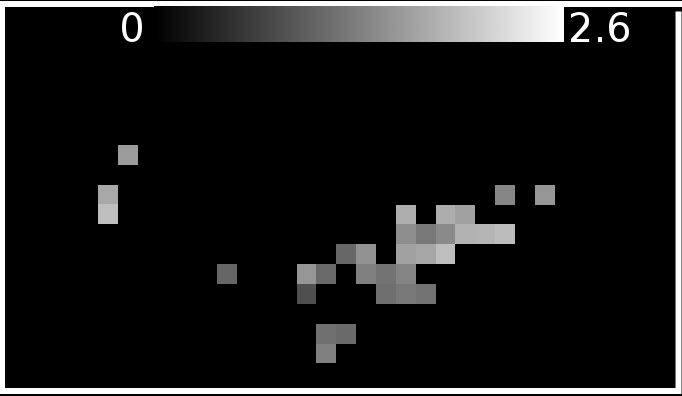
\includegraphics[width=7cm]{images/param_0000_6}}
\subfigure[$\tau_0$, Slice 7]{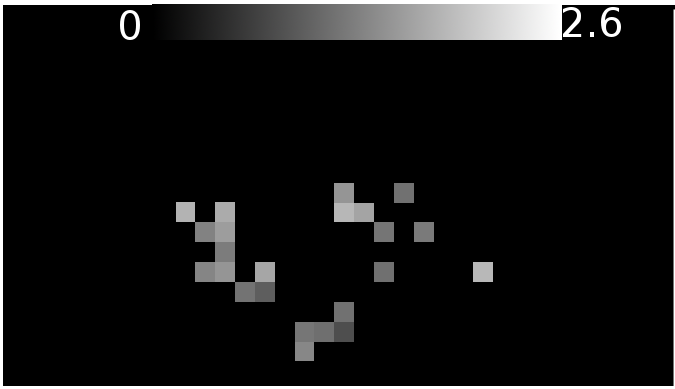
\includegraphics[width=7cm]{images/param_0000_7}}
\subfigure[$\alpha$, Slice 6]{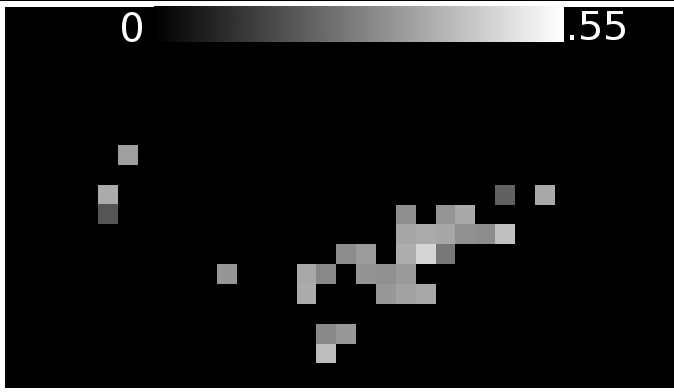
\includegraphics[width=7cm]{images/param_0001_6}}
\subfigure[$\alpha$, Slice 7]{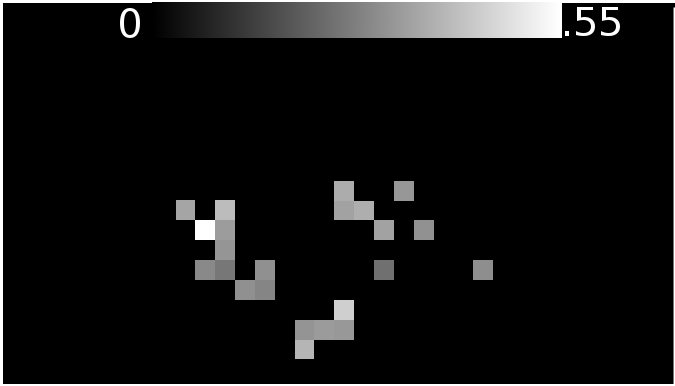
\includegraphics[width=7cm]{images/param_0001_7}}
\subfigure[$E_0$, Slice 6]{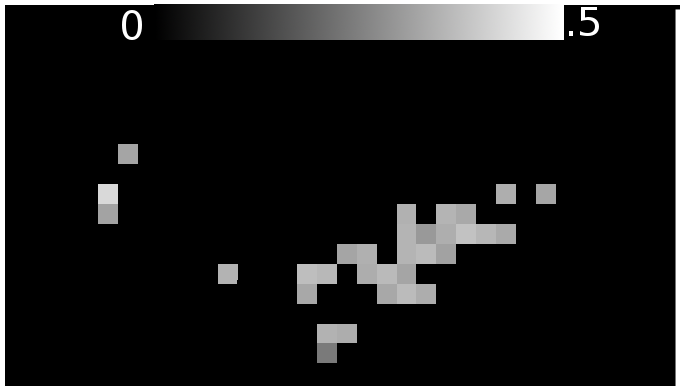
\includegraphics[width=7cm]{images/param_0002_6}}
\subfigure[$E_0$, Slice 7]{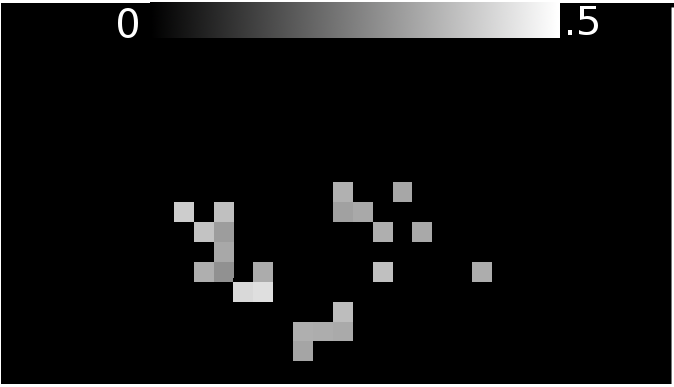
\includegraphics[width=7cm]{images/param_0002_7}}
\subfigure[$V_0$, Slice 6]{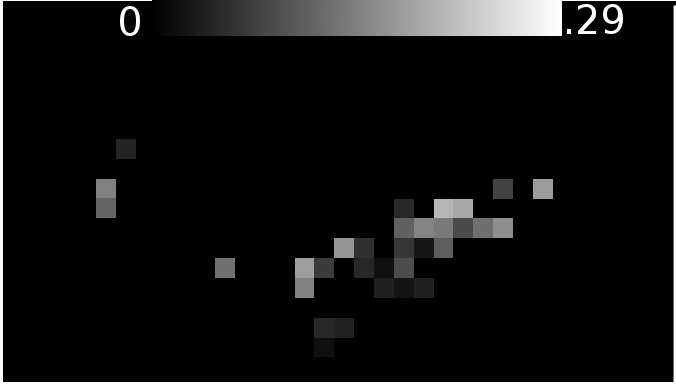
\includegraphics[width=7cm]{images/param_0003_6}}
\subfigure[$V_0$, Slice 7]{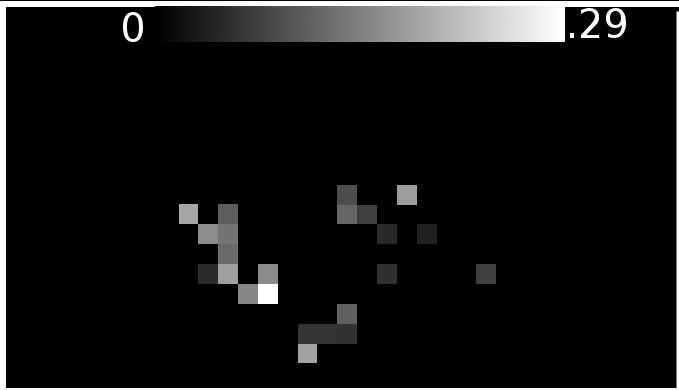
\includegraphics[width=7cm]{images/param_0003_7}}
\end{figure}

\begin{figure}
\centering
\subfigure[$\tau_f$, Slice 6]{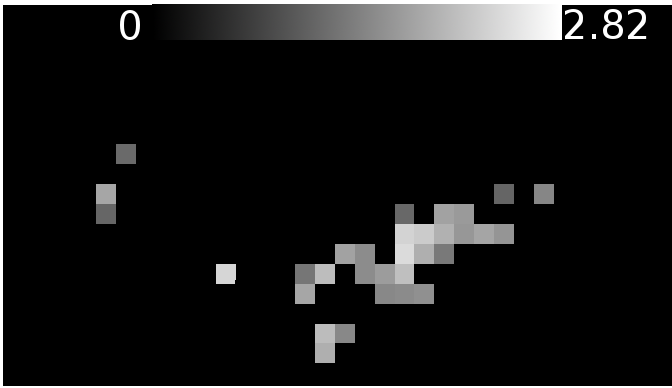
\includegraphics[width=7cm]{images/param_0004_6}}
\subfigure[$\tau_f$, Slice 7]{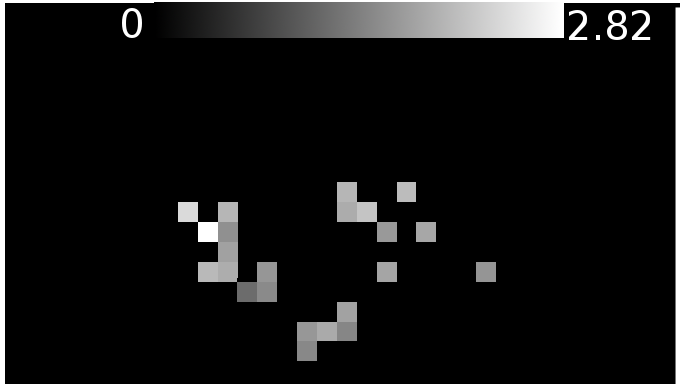
\includegraphics[width=7cm]{images/param_0004_7}}
\subfigure[$\tau_s$, Slice 6]{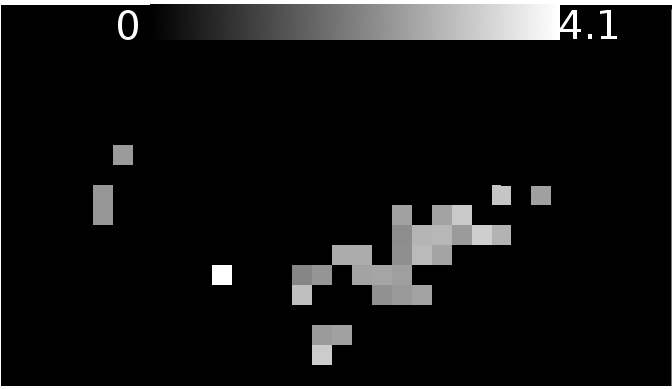
\includegraphics[width=7cm]{images/param_0005_6}}
\subfigure[$\tau_s$, Slice 7]{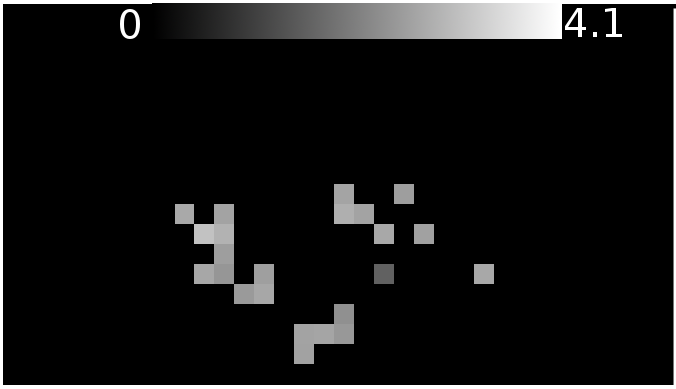
\includegraphics[width=7cm]{images/param_0005_7}}
\subfigure[$\epsilon$, Slice 6]{\includegraphics[width=7cm]{images/param_0006_6}}
\subfigure[$\epsilon$, Slice 7]{\includegraphics[width=7cm]{images/param_0006_7}}
\caption{Parameter Map of two regions of interest ($M.I. > .15$).}
\label{fig:ParameterMap}
\end{figure}

Regions with poor fit cannot have reliable parameter estimates because the input did not meaningfully
correlate input with output. Therefore before creating the maps,
each parameters map was masked to regions with mutual information greater than $.15$. I chose mutual
information over the residual because in the maps comparing regression fitness, the mutual information
maps had more coherency and less randomness. Additionally, in the single voxel tests (\autoref{sec:SingleVoxelReview}) 
there was more separation between the no signal case and the signal case than there was in the 
residual metric. 

\begin{figure}
\centering
\includegraphics[clip=truew,trim=8cm 4cm 8cm 4cm,width=16cm]{images/realhist}
\caption{Histogram of parameters in active regions ($M.I. > .15$).}
\label{fig:FinalHist}
\end{figure}

The parameter maps show consistency parameter across active regions, however, 
the histogram of parameter estimates across all regions with $M.I. > .15$ is the
more interesting result (\autoref{fig:FinalHist}). 

\section{Discussion}
From the maps generated, the similarities to SPM8's results are encouraging. At the 
very least the output of the particle filter seems to meet the quality of SPM. The normalization
of the residual is certainly necessary. Although there is no hard threshold on the 
normalized residual, it would appear that the normalization is providing a reasonable
ordering of regression quality. Mutual information also shows promising results.
Many of the differences between SPM and the particle filter seem to be driven
more by the pre-processing methods than the regression methd. The reason for 
SPM applying such extrensive smoothing is to combat false positives. While this is
extremely important, regions such as \autoref{fig:comp6} show the problem with doing 
so. In all, the particle filter method does very good job of estimating parameters that
fit the measurements; and at the very least this method is a workable, albiet
computationally intensive, alternative to SPM. 
